% \documentclass{memoir}
\documentclass[a5paper,11pt]{memoir}
% TODO try this booklet feature
% https://tex.stackexchange.com/a/17008/133684
% \usepackage{pdfpages}
% \documentclass[17pt]{memoir}
\usepackage[T2A,T1]{fontenc}
\usepackage[utf8]{inputenc}
\usepackage[russian]{babel}
\usepackage{multicol}
\usepackage{hyperref}
\usepackage[math]{anttor}  % set font to Antykwa Torunska
\usepackage[pages=some]{background}
\usepackage{fancyhdr}  % needed to omit chapter name on every page
\usepackage{menukeys}  % for keyboard shortcuts rendered in a special style
\usepackage[symbol]{footmisc} % for dagger footnote
\usepackage{wrapfig}
\usepackage{subcaption} % for displaying figures side by side
\usepackage{geometry}

\usepackage{tikz}
\usetikzlibrary{fadings}

\usetikzlibrary{svg.path}

\newcommand{\Cat}[1][]{%
    \tikz \fill [scale=1ex/500,yscale=-1,#1] svg "m 11.25246,24.361988 c 0.23912,-0.0808 0.32176,-0.0837 0.67212,-0.0237 0.18403,0.0315 0.3323,0.0447 0.57823,0.0515 1.1952,-0.0141 2.21338,-0.25502 3.44291,-0.32574 0.47253,-0.0266 0.67876,-0.062 0.755,-0.1295 0.0169,-0.015 0.0482,-0.0617 0.0696,-0.10391 0.0559,-0.11023 0.15347,-0.18608 0.37982,-0.29528 0.32242,-0.15553 0.71098,-0.4387 0.85097,-0.62015 0.0667,-0.0865 0.2145,-0.3582 0.21546,-0.3962 2.4e-4,-0.01 0.12468,-0.0768 0.27653,-0.14957 8.03377,-8.44437 -1.71627,-12.20777 -0.6037,-17.5505603 1.00879,-1.97094 3.73943,-2.10684 4.55314,0.45219 -0.0403,2.0962104 -2.50861,1.6841704 -1.53097,2.8394004 5.56917,-2.8369304 0.1383,-8.52622041 -3.43984,-4.8528404 -0.96838,1.59509 -0.86918,3.6375704 -0.22968,5.3891904 0.22567,0.60593 0.64255,1.4317699 1.28002,2.5357199 2.07979,3.25143 2.92249,6.18837 -0.25033,8.9793 0.006,-1.5375 -0.10615,-3.34042 -0.31348,-4.63021 -0.50324,-3.08555 -1.43219,-5.02612 -3.00764,-6.2829499 -1.43199,-1.55836 -3.87359,-0.91363 -5.2231904,-1.55155 -0.21256,-0.11129 -0.42204,-0.35791 -0.57147,-0.67275 -0.14564,-0.30684 -0.23687,-0.59548 -0.44939,-1.4216404 -0.30565,-1.24083 -0.72593,-2.36372 -1.54889,-3.2196 -1.04068,-0.78422 -1.85106,-1.76389001 -3.1471798,-2.39562001 -0.0388,-2.4e-4 -0.0887,0.0637 -0.12234,0.15693 -0.0353,0.0978 -0.0537,0.12402 -0.087,0.12402 -0.0136,0 -0.11125,-0.0883 -0.21708,-0.19616 -0.26339,-0.2685 -0.41419,-0.35072 -0.48987,-0.2671 -0.049,0.0542 -0.0243,0.16781 0.15688,0.71958 0.0926,0.28195 0.17244,0.55204001 0.17749,0.60020001 0.0178,0.17003 -0.0266,0.20257 -0.43563,0.31879 -0.39825,0.11317 -0.53254,0.18289 -0.84154,0.43695 -0.20381,0.16758 -0.46294,0.42123 -0.67577,0.66151 -0.20774,0.23452 -0.25382,0.32963 -0.44934,0.92755 -0.0847,0.25903 -0.17345999,0.50415 -0.19723999,0.54471 -0.0529,0.0902 -0.16694,0.23026 -0.35654,0.4377 -0.079,0.0864 -0.16068,0.19058 -0.18158,0.23151 -0.12332,0.24151 -0.10769,0.50979 0.0389,0.66688 0.0719,0.0771 0.0935,0.13288 0.0937,0.24251 2.7e-4,0.11897 0.061,0.22556 0.20314,0.35654 0.12157,0.1120204 0.12602,0.1188204 0.14186,0.2172204 0.0188,0.11646 0.0466,0.17766 0.13465,0.29572 0.10602999,0.14221 0.28299999,0.21757 0.85137999,0.36252 1.47374,0.26187 1.15133,1.79944 0.86874,2.58682 -0.30255,0.8417499 -0.35649,1.0615899 -0.3553,1.4481599 9e-4,0.28839 0.024,0.41722 0.14726,0.82246 0.46047,2.2245 2.41886,3.55693 2.70957,5.55234 -0.31468,1.22946 -0.32413,2.29536 -0.6523,3.61533 -0.0224,0.0447 -0.1218,0.0898 -0.36153,0.16413 -0.47798,0.14825 -0.61257,0.21207 -0.70583,0.33471 -0.20215,0.5016 0.0411,1.13393 0.57021,1.18881 0.0657,0.006 0.11954,0.0139 0.11954,0.0187 0,0.005 -0.0471,0.0576 -0.10465,0.11749 -0.122,0.12686 -0.1867,0.23098 -0.21905,0.35249 -0.0674,0.2532 0.0252,0.56505 0.19758,0.6651 0.0375,0.0218 0.11289,0.0511 0.16746,0.065 0.80648,0.12239 1.8985598,0.31913 2.4586398,-0.21764 0.12494,-0.12124 0.17461,-0.18333 0.2257,-0.28217 0.0763,-0.1476 0.14617,-0.36041 0.20991,-0.63935 0.0544,-0.23797 0.0774,-0.28939 0.12972,-0.28939 0.0211,0 0.17271,0.0332 0.337,0.0738 0.88672,0.1598 1.09925,0.13215 2.04551,0.17731 l 0.0962,0.0833 c 0.0529,0.0458 0.094,0.0887 0.0914,0.0952 -0.003,0.007 -0.0606,0.0579 -0.1288,0.11416 -0.22109,0.18234 -0.39882,0.419 -0.46096,0.6138 -0.0329,0.10303 -0.048,0.28529 -0.0328,0.39572 0.0332,0.24185 0.17651,0.42025 0.44426,0.55304 0.6004504,0.18818 1.0365604,0.13982 1.7004104,-0.0724 z";%
}

\newcommand{\Dolphin}[1][]{%
    \tikz \fill [scale=1ex/500,yscale=-1,#1] svg "M 240,792 C 236.7964,782.29301 227.32595,769.18429 218.95458,762.8695 C 210.58318,756.55478 193.07658,741.91749 180.05096,730.34232 L 156.36806,709.29648 L 141.17601,721.53827 C 132.82037,728.27131 116.86485,736.20204 105.71929,739.16215 C 94.57372,742.12228 76.825609,750.15889 66.279001,757.02126 C 42.749986,772.33104 35.286663,768.91329 39.793018,744.89235 C 49.786747,691.62137 86.56609,637.47901 123.0161,622.38091 C 133.32885,618.10921 138.97291,610.6592 143.54681,595.28094 C 156.31386,552.35575 185.13223,485.10659 210.50659,439.02657 C 285.62548,302.61033 377.12604,221.91941 502.90248,181.17368 L 545.4538,167.38902 L 523.9559,153.16241 C 512.13201,145.33777 493.01385,137.67119 481.47106,136.12559 C 441.72739,130.80384 454.06939,100.38528 495.97229,100.38528 C 525.1625,100.38528 588.32595,117.28333 612.47161,131.55225 C 631.20187,142.62093 638.05903,143.46536 711.12662,143.70143 C 826.20118,144.07318 875.39668,159.99674 936.18511,216.548 C 957.70508,236.568 977.32088,249.47994 997.76359,257.08148 C 1037.1384,271.7229 1050.5601,280.83354 1050.5601,292.92001 C 1050.5601,304.96929 1043.1872,306.72156 979.27795,309.86153 C 937.41314,311.91844 922.54209,315.36478 870.35529,335.10414 C 837.1142,347.67736 806.21965,359.09969 801.70072,360.48707 C 797.18181,361.87448 788.5903,373.11962 782.60856,385.47631 C 769.33352,412.89887 732.8923,450.74636 708.71893,462.21739 C 687.47223,472.29962 645.39097,477.58347 636.22902,471.31951 C 626.59388,464.73198 633.77941,451.7414 651.00501,444.60631 C 668.76327,437.2506 688.54805,412.99772 693.73219,392.22992 L 697.39133,377.57125 L 659.92998,381.16743 C 639.32621,383.14537 594.48504,391.40641 560.28293,399.5254 C 408.28252,435.60753 289.59011,503.28314 223.04114,591.81285 L 199.83212,622.68772 L 222.77838,652.2359 C 249.05732,686.07569 265.30365,731.48301 265.30365,771.09095 C 265.30365,810.05728 250.10447,822.61677 240,792 M 885.93164,242.20228 C 889.77822,235.9783 875.83562,229.90601 868.33788,234.5399 C 865.37262,236.37259 864.25805,239.99423 865.8612,242.58811 C 869.72788,248.8446 881.97191,248.60916 885.93164,242.20228 z";%
}

\pgfdeclareradialshading{myfadingraw}{\pgfpointorigin}{
  color(0pt)=(pgftransparent!5); color(21bp)=(pgftransparent!10);
  color(25bp)=(pgftransparent!100); color(50bp)=(pgftransparent!100)}%
\pgfdeclarefading{side shaded}{\pgfuseshading{myfadingraw}}%

%%%%%%%%%%%%%%%%%%%%%%%%%%%%%%%%%%%%%%%%%%%%%%%%%%%%%
% this is to implement blurry text as shown here:
% https://tex.stackexchange.com/a/571691/133684
\newcommand{\blurry}[2]{
% Draw the blur
\foreach \a in {0,5,...,360}
{   \foreach \r in {0,.1,...,1}
    {   \draw [black, opacity=0.02] node at (\a:\r ex) {#1};
    }
}
% Draw the solid text
\draw [#2, opacity=1.0] node at (0,0) {#1};
}
%%%%%%%%%%%%%%%%%%%%%%%%%%%%%%%%%%%%%%%%%%%%

% \usepackage{nextpage} % needed for \cleartoevenpage, to ensure the last page/cover will fold as we need

% this is to have proper quotes for Russian text <<  >> (not " ")
\usepackage{csquotes}

% Syntactic sugar: a command for direct speech of various characters - it will be rendered as
% a quote with an emphasis. For quoting non-speech, use \textquote
\newcommand{\say}[1]{\emph{\textquote{#1}}}


% this is used to set the metadata of the PDF itself
% see https://en.wikibooks.org/wiki/LaTeX/Hyperlinks#Customization
\hypersetup{
    pdftitle={0! Книга для добрых детей},
    pdfauthor={Alex Railean},
    pdfsubject={Стихотворения для детей},
    % pdfcreator={Creator},   % creator of the document
    % pdfproducer={Producer}, % producer of the document
    pdfkeywords={стихи, образование}, % list of keywords
    pdfpagelayout=TwoPageRight, % display as 2 columns by default, useful during development and testing
}



% EXPERIMENT with this to manipulate margin size
% https://tex.stackexchange.com/a/378157/133684
% \setlrmarginsandblock{3.5cm}{2.5cm}{*}
% \setulmarginsandblock{2.5cm}{*}{1}
% \checkandfixthelayout 


\title{\begin{otherlanguage*}{russian}
0! Книга для добрых детей
\end{otherlanguage*}}  
% \author{Alex Railean}
\author{}
% \date{November 2022}


% This is necessary to remove chapter titles from every page, which would be shown otherwise
% https://stackoverflow.com/a/62250429/27342
\pagestyle{fancy}
\fancyhead[R]{\thepage}
\fancyhead[L]{}
\renewcommand{\headrulewidth}{0pt}
\fancyfoot{}
%%%%%%%%%%%%%%%%%%%%%%%%%%%%%%%%%%%%%%%%%%%%



% Adjust poem titles, so they are bigger and thicker
\renewcommand{\PoemTitlefont}{%
\normalfont\huge\bfseries\centering}


% Set the right margin to 1cm and the top margin to 1.5cm.
% https://tex.stackexchange.com/a/378157/133684
\setlrmarginsandblock{*}{1cm}{1}
\setulmarginsandblock{1.5cm}{*}{1}
\checkandfixthelayout
\begin{document}
% redefine font size 14 as 14.5 using this method, because doing it at the very top of the file only lets us choose between 12 14 17...
% https://tex.stackexchange.com/questions/323443/how-to-specify-intermediate-font-sizes-in-memoir-class
% \fontsize{15pt}{14pt}\selectfont

\date{} % so no date is shown under the title
\maketitle
\begin{center}
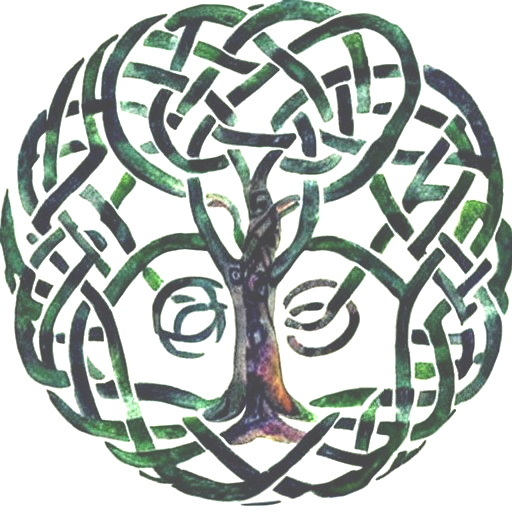
\includegraphics[height=7cm]{images/tree-cover} 
\end{center}
\thispagestyle{empty}
\newpage
\thispagestyle{empty}  % to not have a page# here

\selectlanguage{russian}
% \backgroundsetup{scale=1,opacity=1,angle=0,contents={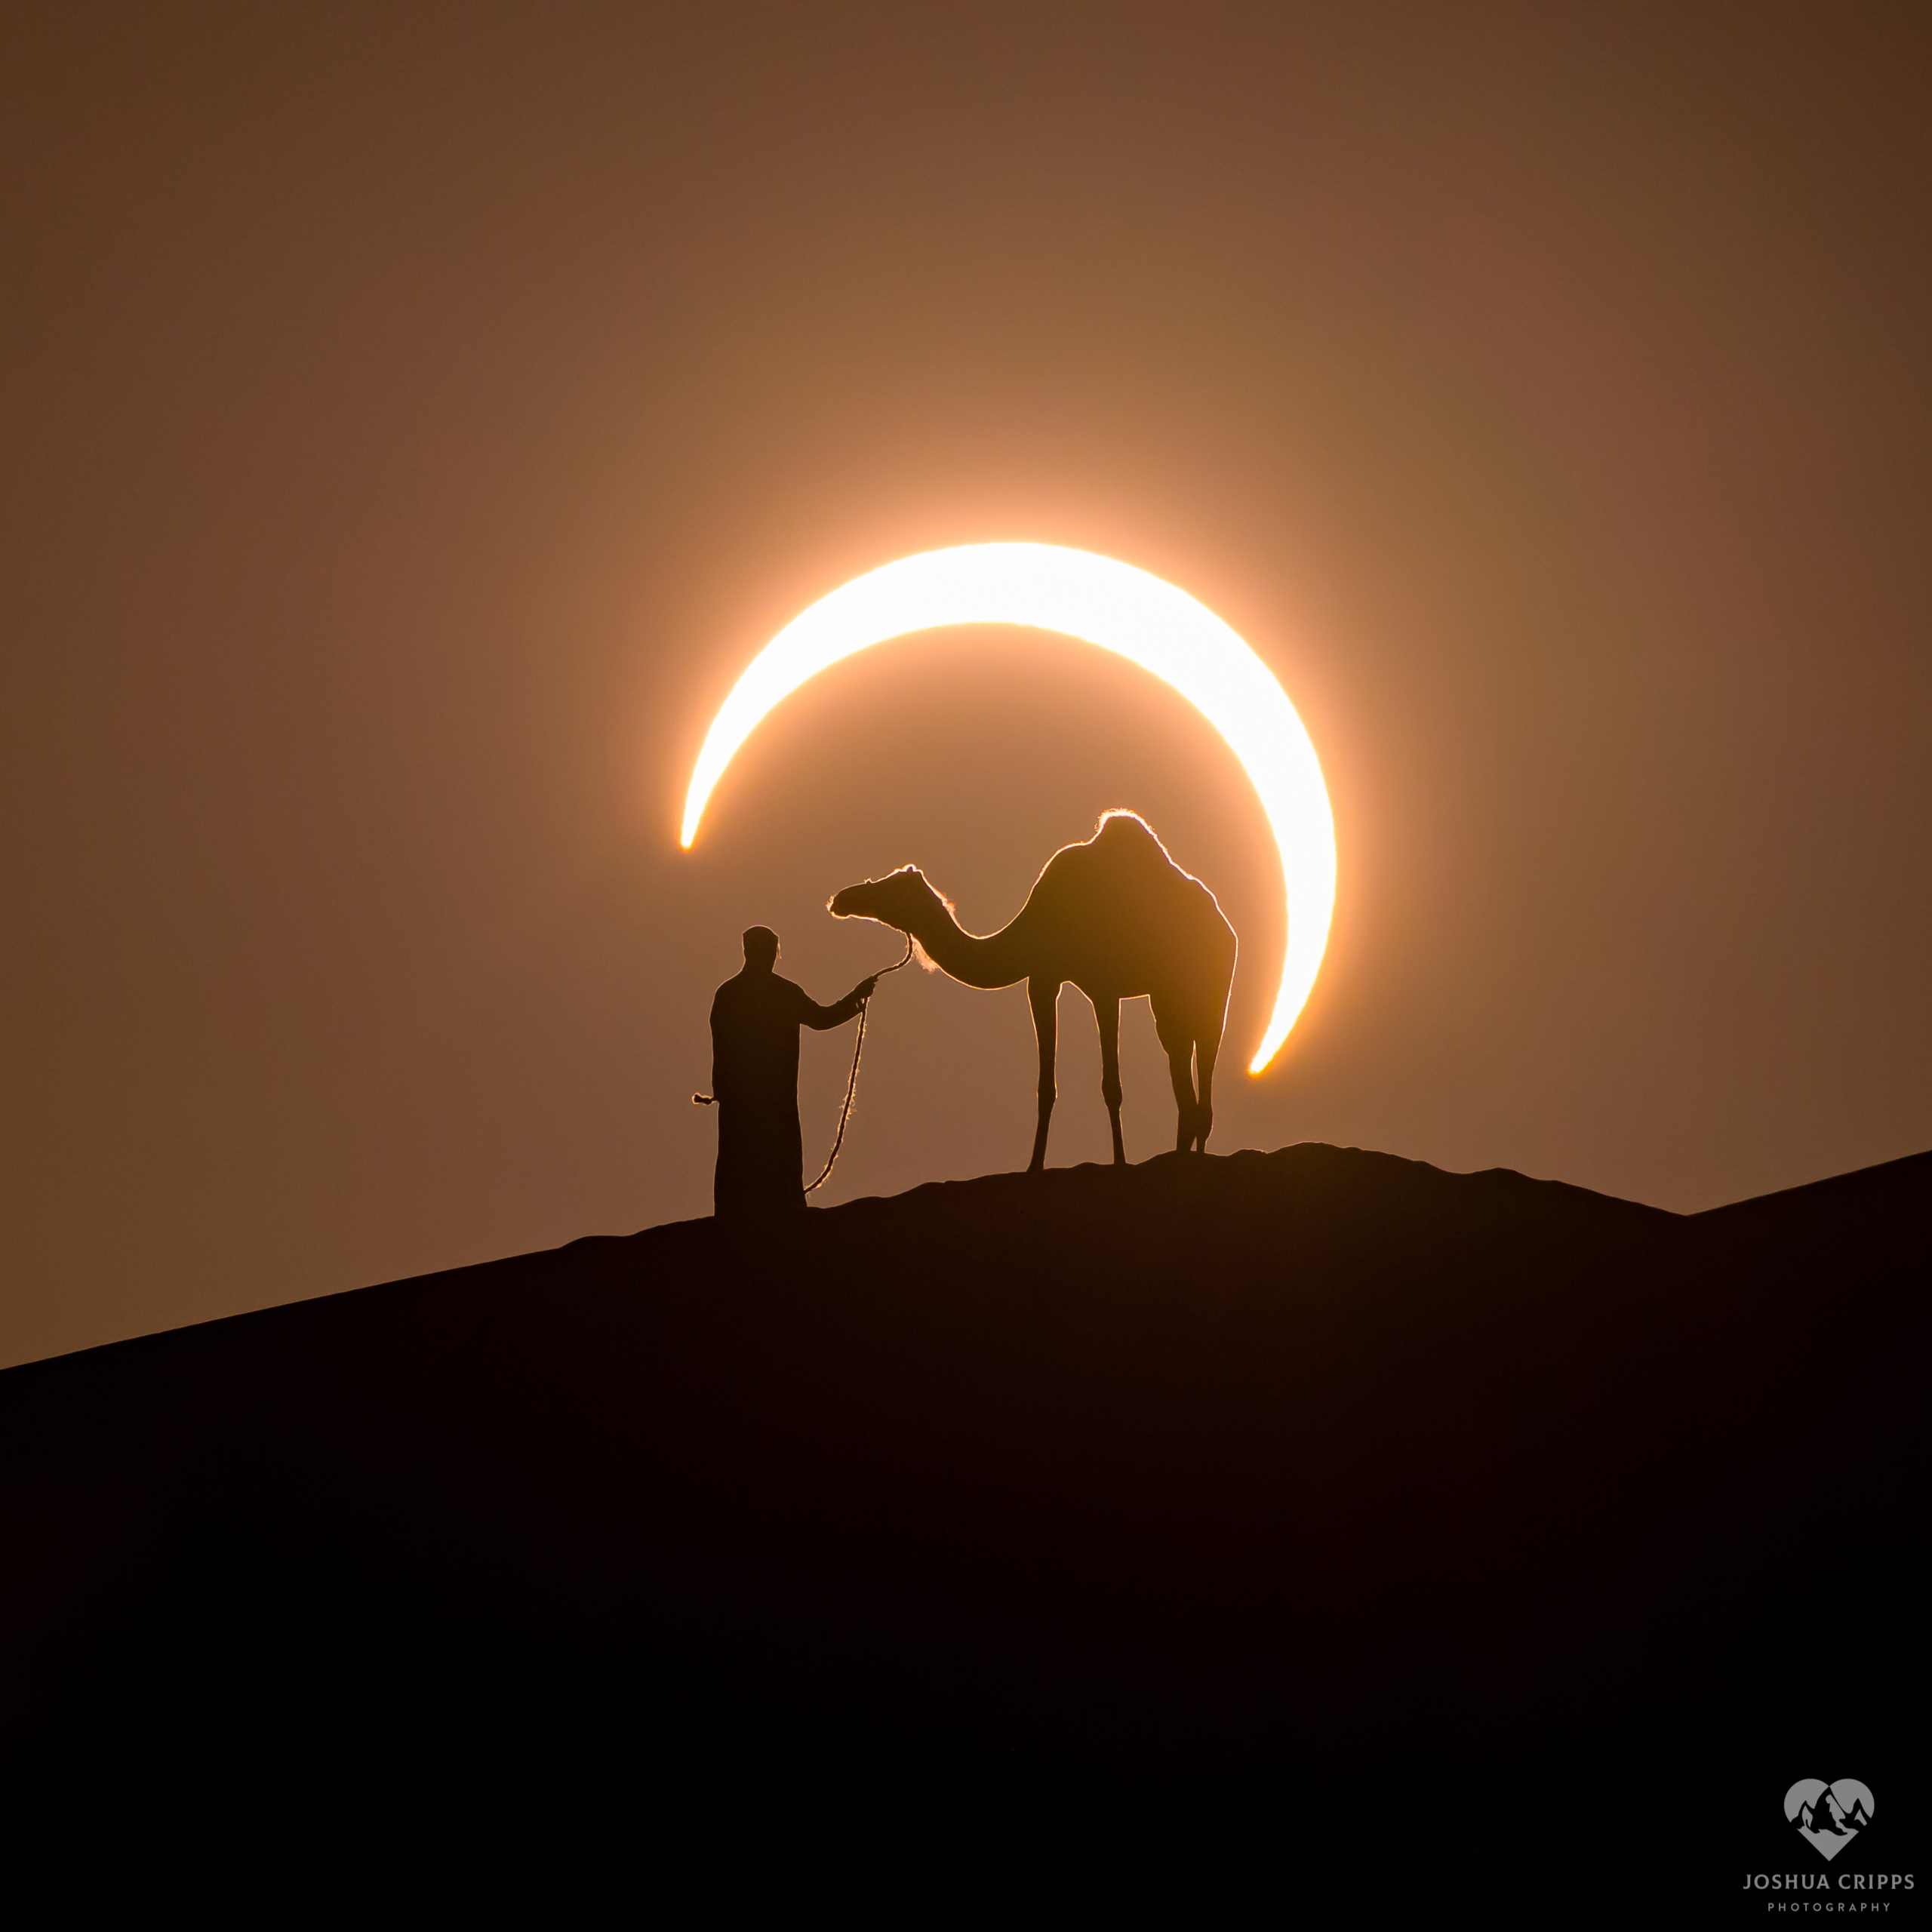
\includegraphics[width=\paperwidth,height=\paperheight]{eclipse.jpg}}}

\clearpage
% uncomment the line below to hide page number 
% \thispagestyle{empty}
\hfill

\backgroundsetup{scale = 1, angle = 0, opacity = 0.02, contents = {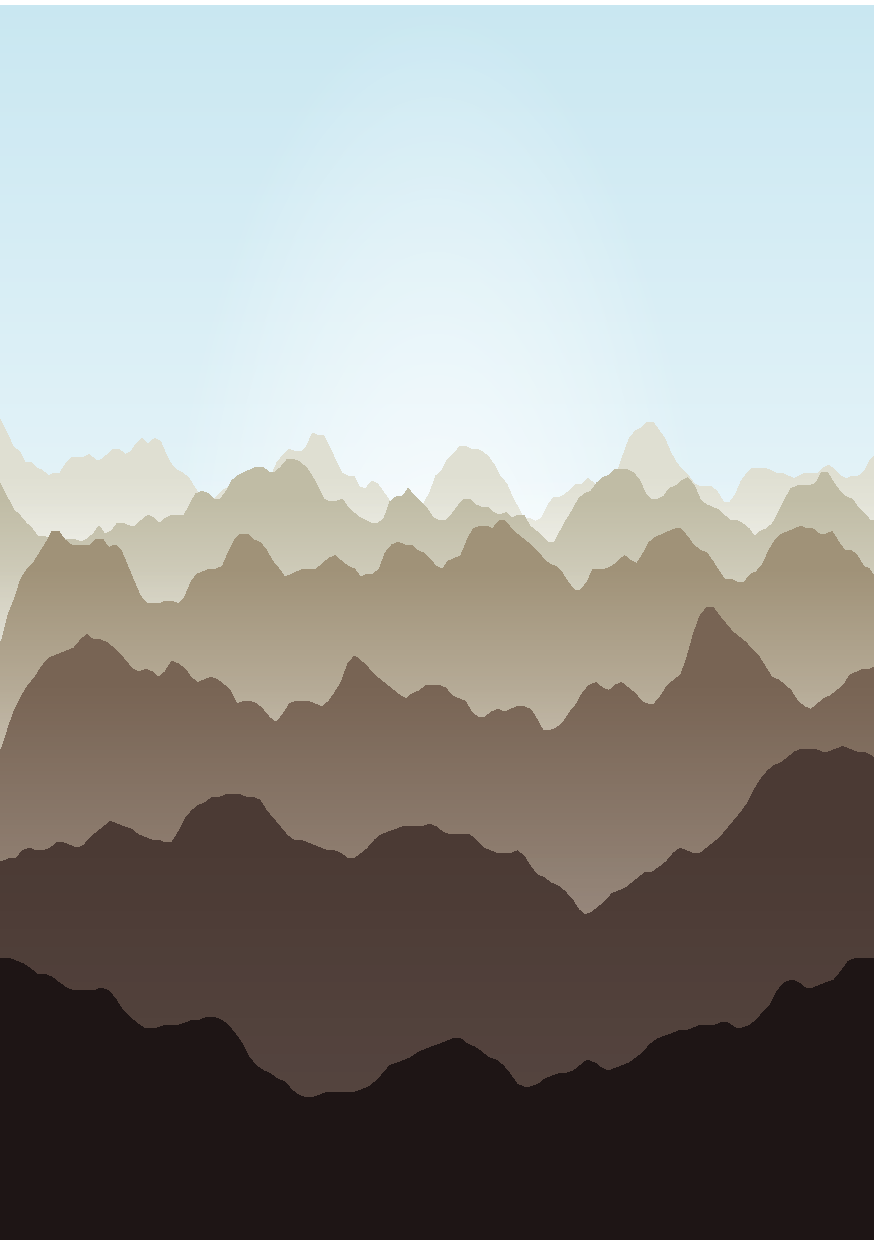
\includegraphics[width = \paperwidth, height = \paperheight] {images/mountains.pdf}}}
\BgThispage

\section{От автора}
\small{
Когда я учился во втором классе, на одном из уроков мы изучали некое стихотворение\footnote{Vasile Alecsandri, ``Adio Moldovei''; в оригинале троеточия нет, в учебнике была сокращенная версия.}, которое заканчивалось троеточием. Я спросил практиканта, который вёл урок, об этих точках. Его точного ответа я не помню, но помню свою интерпретацию - незавершенная мысль, чего-то не хватает, что-то отсутствует. Раз не хватает - значит нужно дополнить! Я сочинил свою концовку, думая что это очередное задание для учеников. Это был очень интересный процесс, буд-то я получил \textit{автор}изацию на продолжение работы, приглашение на диалог с автором, и его доверие - довести дело до конца, не завалив задачу.


Цель этой книги, дать возможность каждому быть не только потребителем информации, но и создателем. Книга распространяется по лицензии Creative commons (cc-by), которая позволяет менять её текст, иллюстрации, шрифты и дизайн - всё! Кое-где нужно улучшить рифму - меняй! Хочешь другую картинку, чтобы кошка была чёрной а не рыжей - меняй! Хочешь распечатать книгу с более крупным текстом, и в твёрдом переплёте - делай это! По-твоему диджериду звучит совсем не так - переписывай!
}
\newpage

\addto\captionsrussian{ 
}
% so the table of contents itself is not shown in the table of contents
\begin{KeepFromToc}
  \tableofcontents
\end{KeepFromToc}

\backgroundsetup{scale = 1, angle = 0, opacity = 0.45, contents = {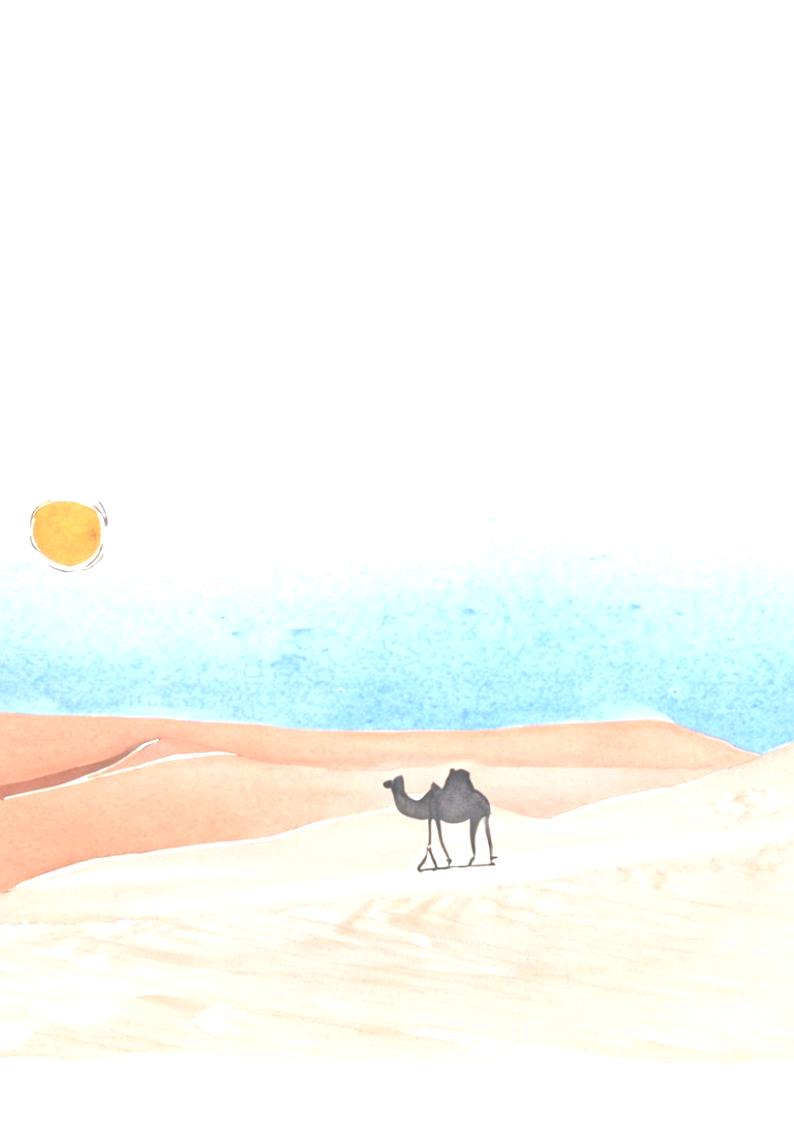
\includegraphics[width = \paperwidth, height = \paperheight] {images/camel}}}
\BgThispage


\thispagestyle{empty}  % hide page number
\newpage
\thispagestyle{empty}

\pagenumbering{arabic}  % so the second page begins with #1

% Show only the LEFT side of a landscape A4 drawing
\backgroundsetup{scale = 1, angle = 0, opacity = 1, contents = {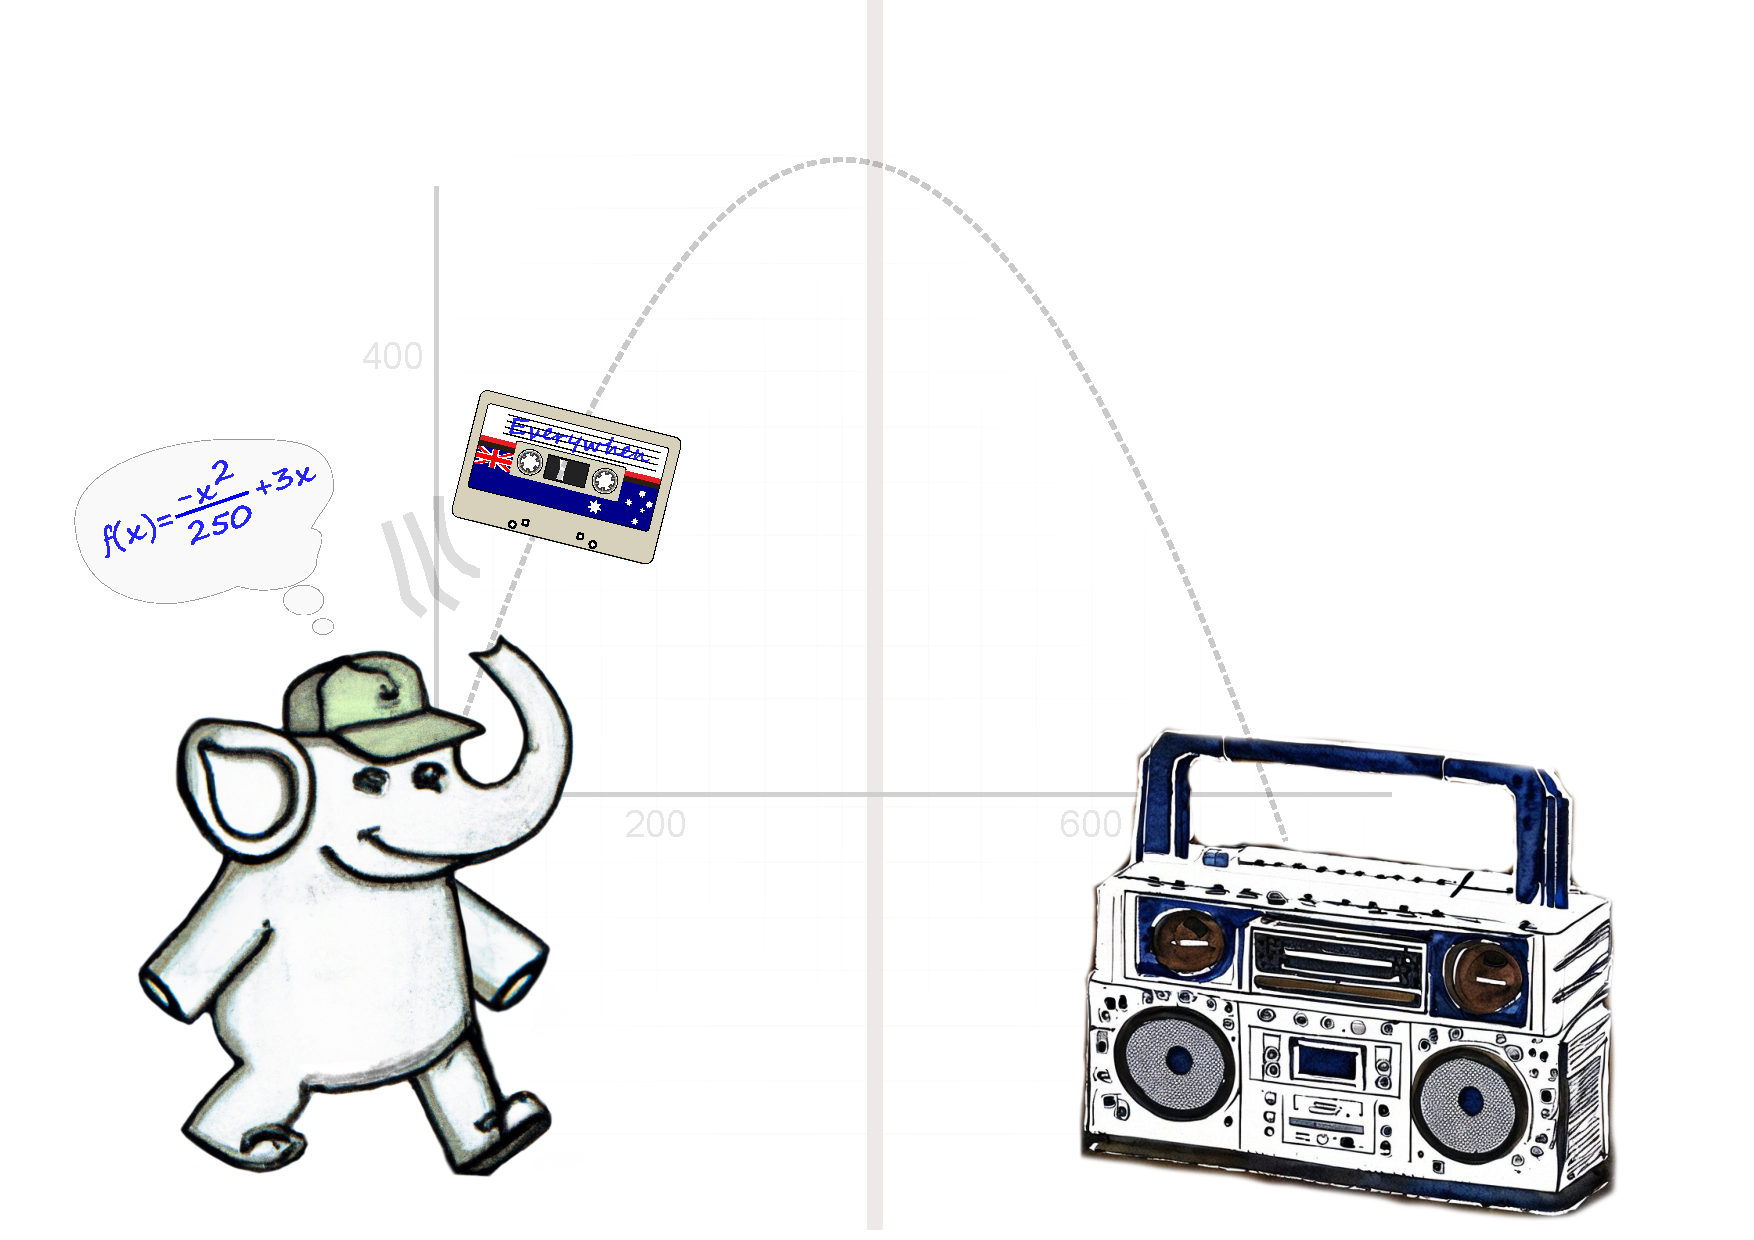
\includegraphics[width = \paperwidth, height = \paperheight,trim={0 0 148mm 0},clip] {images/parabola-tape-recorder}}}
\BgThispage
% This is to move the poem to the right side, when printed
% as a booklet

\clearpage
% uncomment the line below to hide page number 
% \thispagestyle{empty}
\hfill
\clearpage

% Show only the RIGHT side of a landscape A4 drawing
\backgroundsetup{scale = 1, angle = 0, opacity = 1, contents = {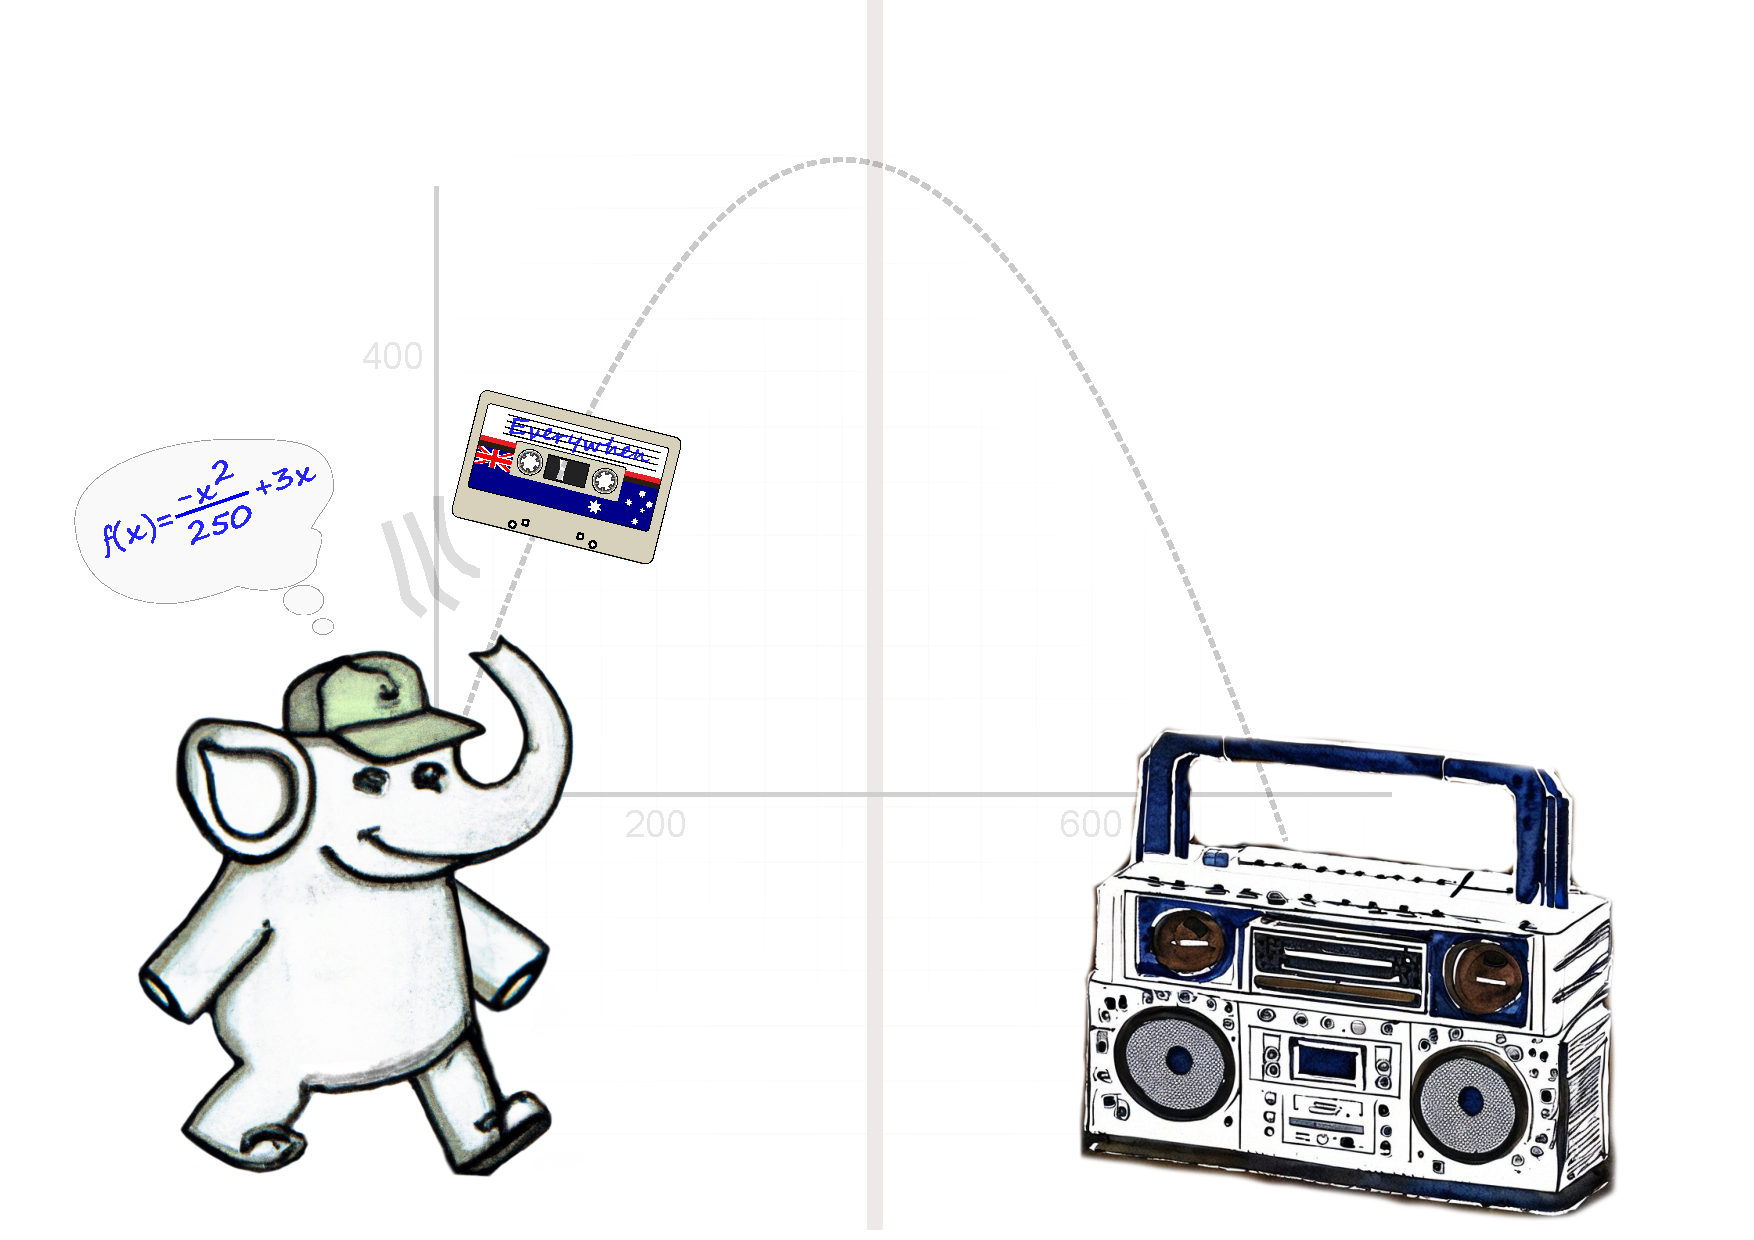
\includegraphics[width = \paperwidth, height = \paperheight,trim={148mm 0 0 0},clip] {images/parabola-tape-recorder}}}
\BgThispage

\PlainPoemTitle
\PoemTitle{Харитон и хакатон}
\settowidth{\versewidth}{ступеньки под весом скрипят и трещат ---}
\begin{verse}[\versewidth]
Жил-был добрый слон,\\
И звали его Харитон.
\end{verse}

\begin{verse}[\versewidth]
Прихватив клавиатуру под мышку,\\
по комнате шёл он вприпрыжку.\\
Хоботом, словно ракету,\\
подкинул он в воздух кассету.\\
А та, как диктует закон,\\
параболой --- в магнитофон!
\end{verse}
% \newpage

\begin{verse}[\versewidth]
Летит и порхает как бабочка слон,\\
жужжит на плече его магнитофон,\\
ступеньки под весом начинают трещать --- \\
слона не легко на себе удержать!
\end{verse}

\newpage
% \begin{center}
% 
\includegraphics[height=11cm]{images/hariton.png} 
% \end{center}


% hackathon left side
\backgroundsetup{scale = 1, angle = 0, opacity = 1, contents = {\includegraphics[width = \paperwidth, height = \paperheight,trim={0 0 148mm 0},clip] {images/hackathon-group}}}
\BgThispage



\begin{verse}[\versewidth]
И радость его не находит границы,\\
смеются в слоне даже микрочастицы!\\
Ведь знает, ведь знает,\\
наш слон, Харитон,\\
что путь приведёт его на Хакатон!
\end{verse}
% \newpage

% hackathon right side


\begin{verse}[\versewidth]
Он встретится там со своими друзьями,\\
с питоном, пингвином, гну, и с китами!\\
И вместе они порешают задачи,\\
чтоб мир вдруг стал лучше,\\
чтоб мир жил иначе!
\end{verse}


\begin{verse}[\versewidth]
Чтоб дети планеты могли без забот\\
глядеть в телескоп, в микроскоп --- круглый год!\\
Чтоб насмотревшись Вселенной красот,\\
в жизни достигли новых высот.
\end{verse}

\newpage
\hfill
\backgroundsetup{scale = 1, angle = 0, opacity = 1, contents = {\includegraphics[width = \paperwidth, height = \paperheight,trim={148mm 0 0 0},clip] {images/hackathon-group}}}
\BgThispage

\newpage

\renewcommand{\thefigure}{\arabic{figure}}

\newgeometry{margin=0in}
\begin{figure}[t]
  \begin{subfigure}{.5\paperwidth}
    \centering
    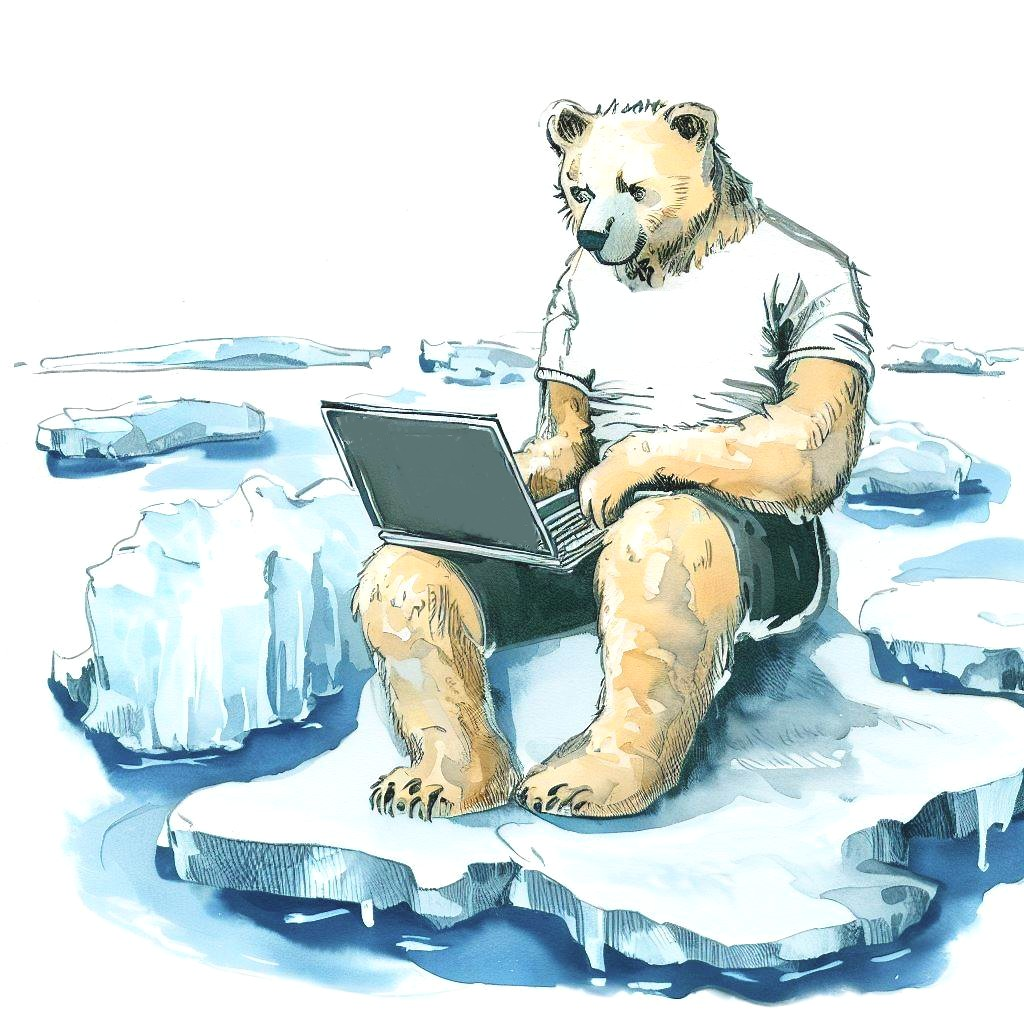
\includegraphics[width=.8\linewidth]{images/bear-laptop.jpg}
    \caption{Сбор телеметрии с сенсоров}
  \end{subfigure}%
  \begin{subfigure}{.5\paperwidth}
    \centering
    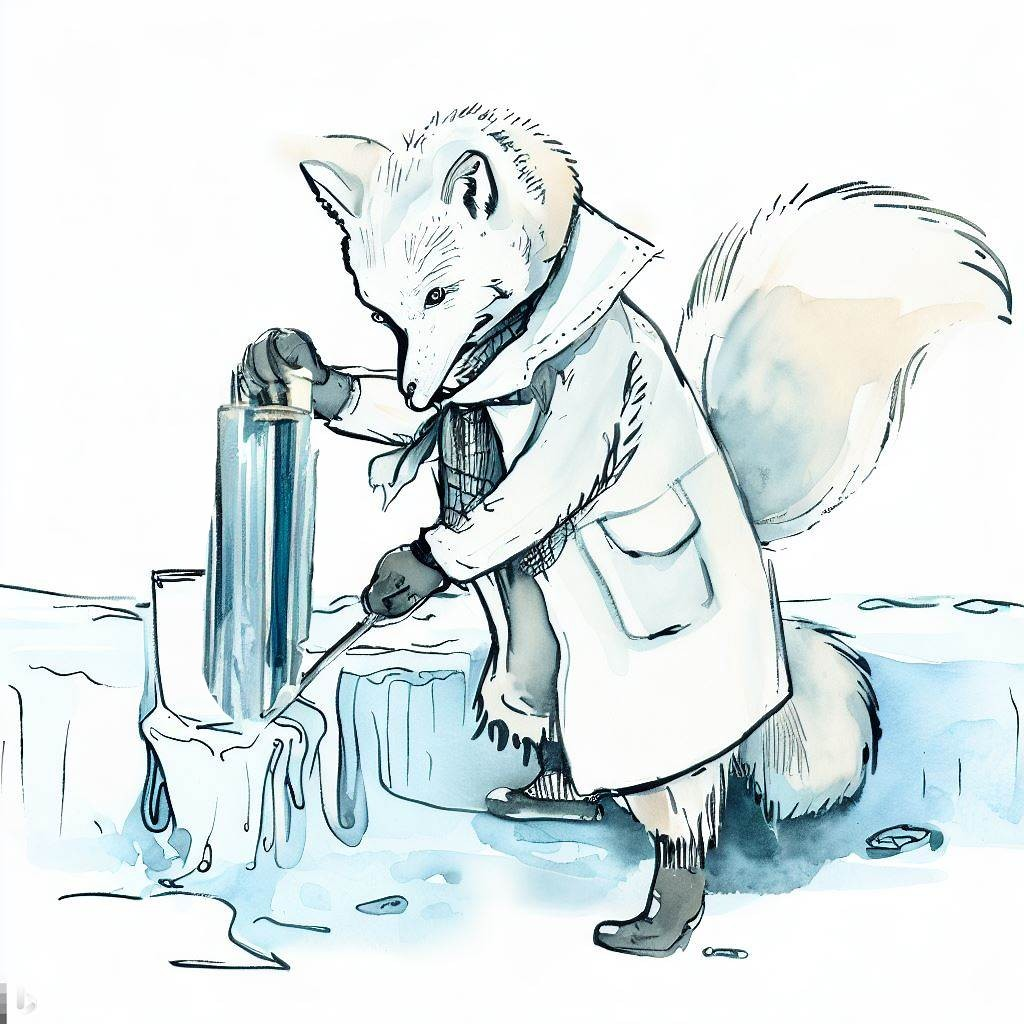
\includegraphics[width=.8\linewidth]{images/fox-ice-core.jpg}
    \caption{Экстракция ледяного керна}
  \end{subfigure}
  \caption{Решение проблемы глобального потепления}
\end{figure}
% \restoregeometry

\vspace{-0.5cm}
\begin{figure}%[h]
  \begin{subfigure}{.33\paperwidth}
    \centering
    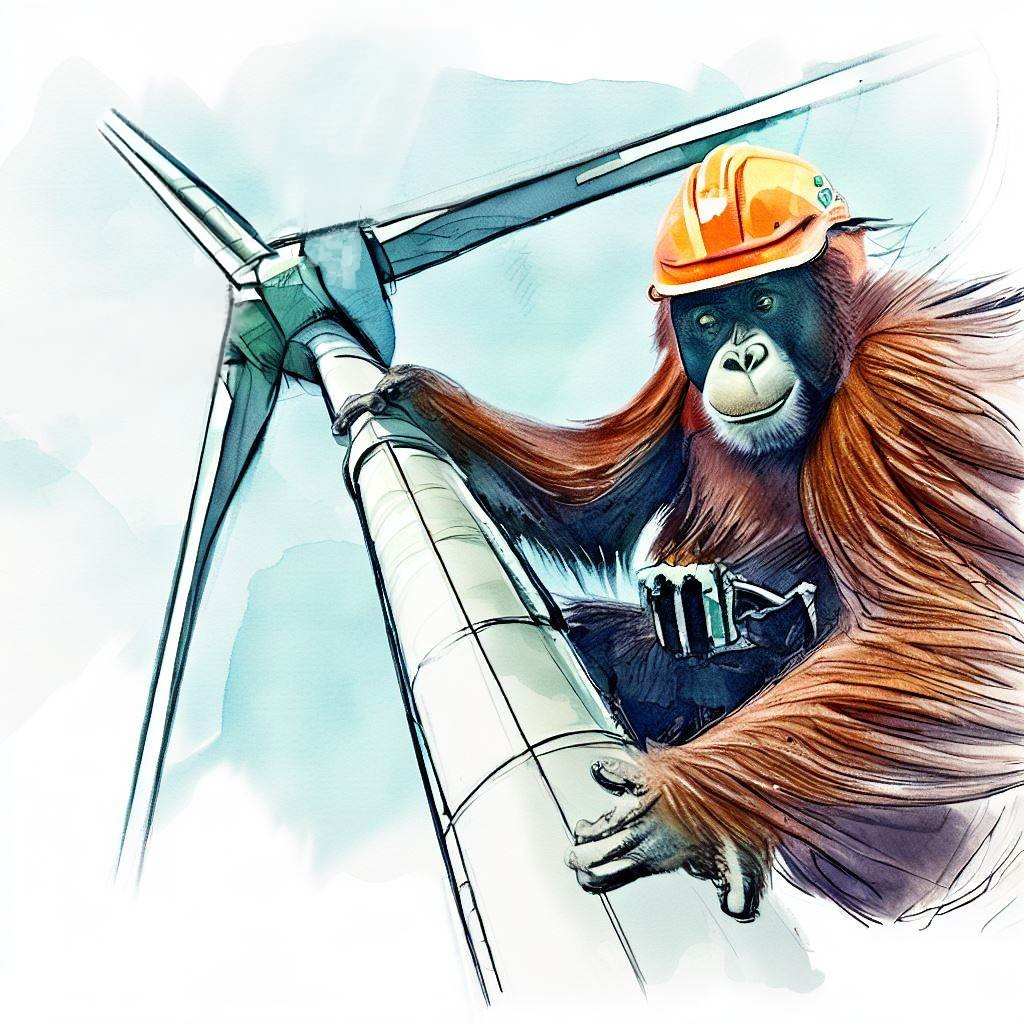
\includegraphics[width=.8\linewidth]{images/orangutan-climber.jpg}
    \caption{Ремонт генератора}
  \end{subfigure}%
  \begin{subfigure}{.33\paperwidth}
    \centering
    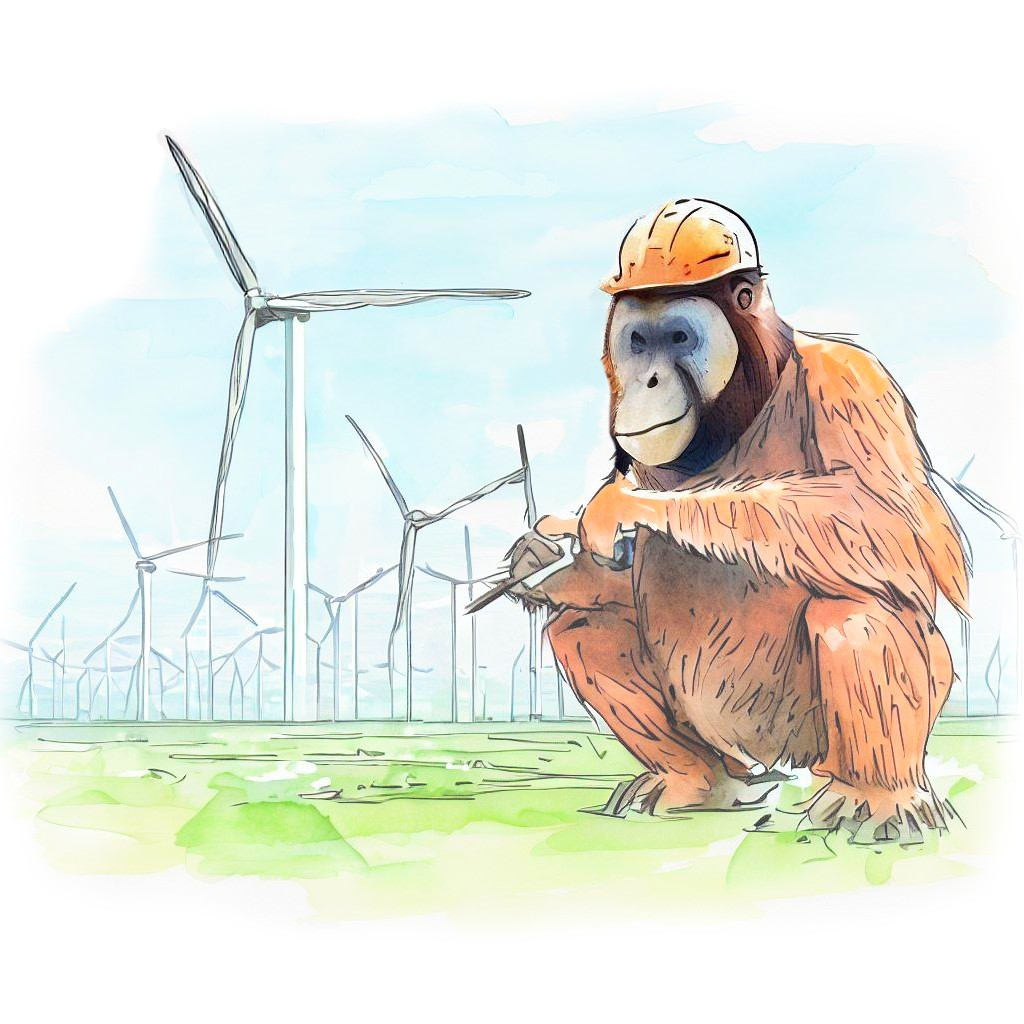
\includegraphics[width=.8\linewidth]{images/orangutan-windfarm.jpg}
    \caption{Ветропарк}
  \end{subfigure}%
  \begin{subfigure}{.33\paperwidth}
    \centering
    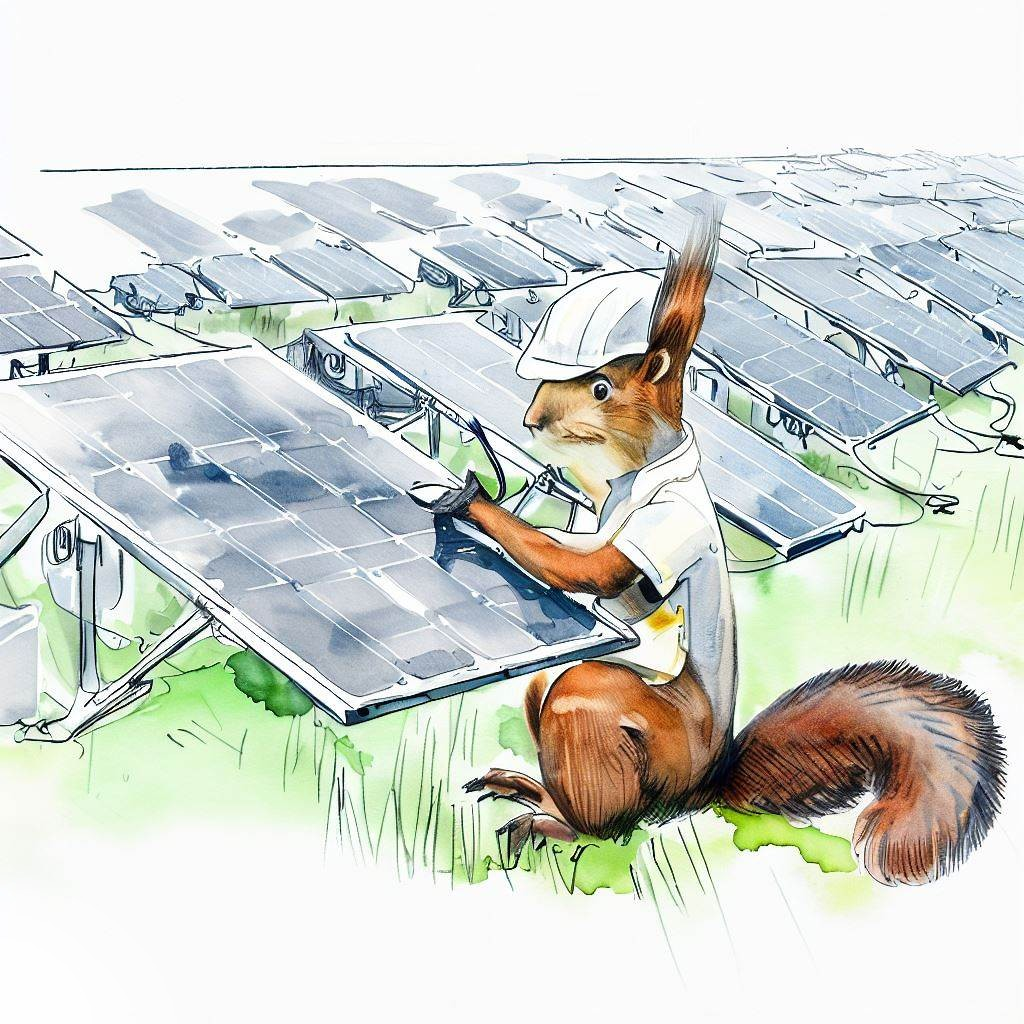
\includegraphics[width=.8\linewidth]{images/squirrel-solar-panel.jpg}
    \caption{Солнечные панели}
  \end{subfigure}
  \caption{Возобновляемая энергия}
\end{figure}

\vspace{-5.5cm}

% \setlength{\intextsep}{0pt} % Reduce space between figures
\begin{figure}[h]
  \begin{subfigure}{.5\paperwidth}
    \centering
    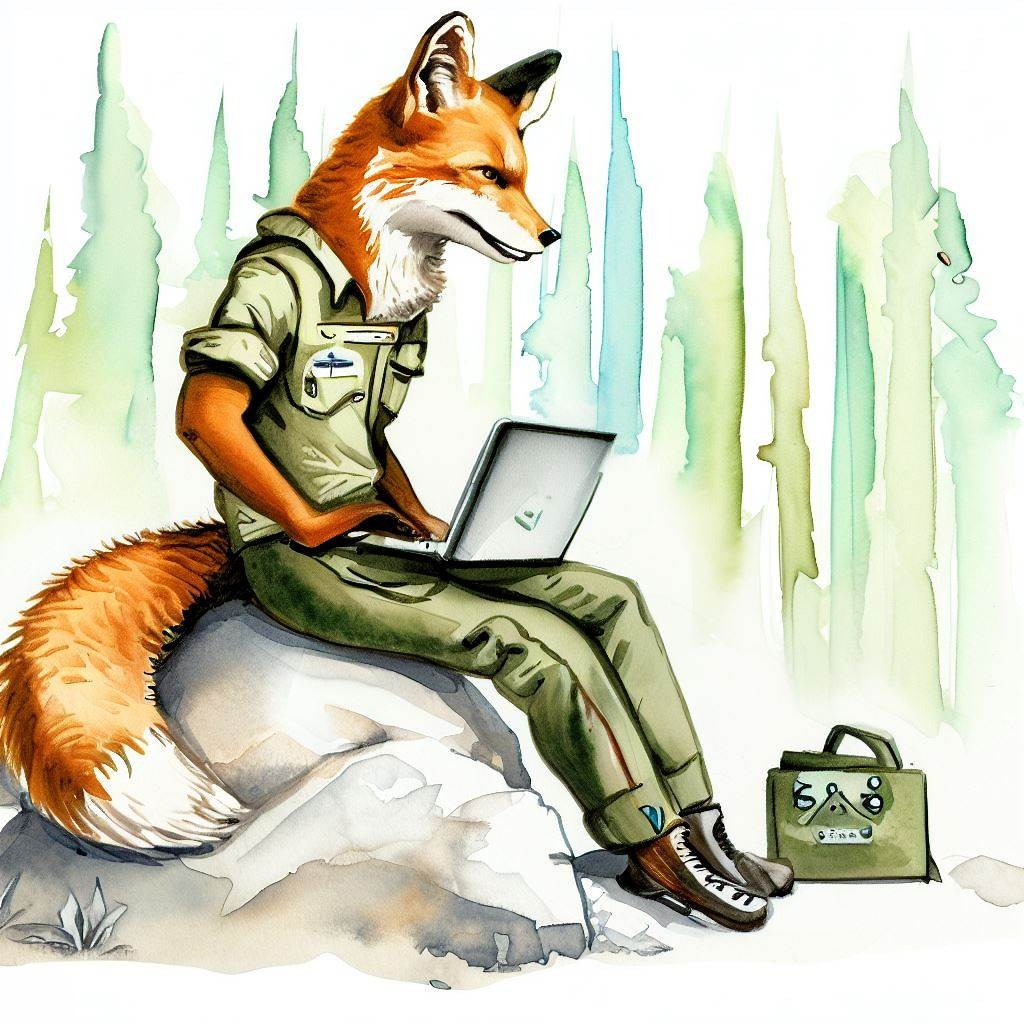
\includegraphics[width=.8\linewidth]{images/fox-ranger.jpg}
    \caption{Администратор заповедника}
  \end{subfigure}%
  \begin{subfigure}{.5\paperwidth}
    \centering
    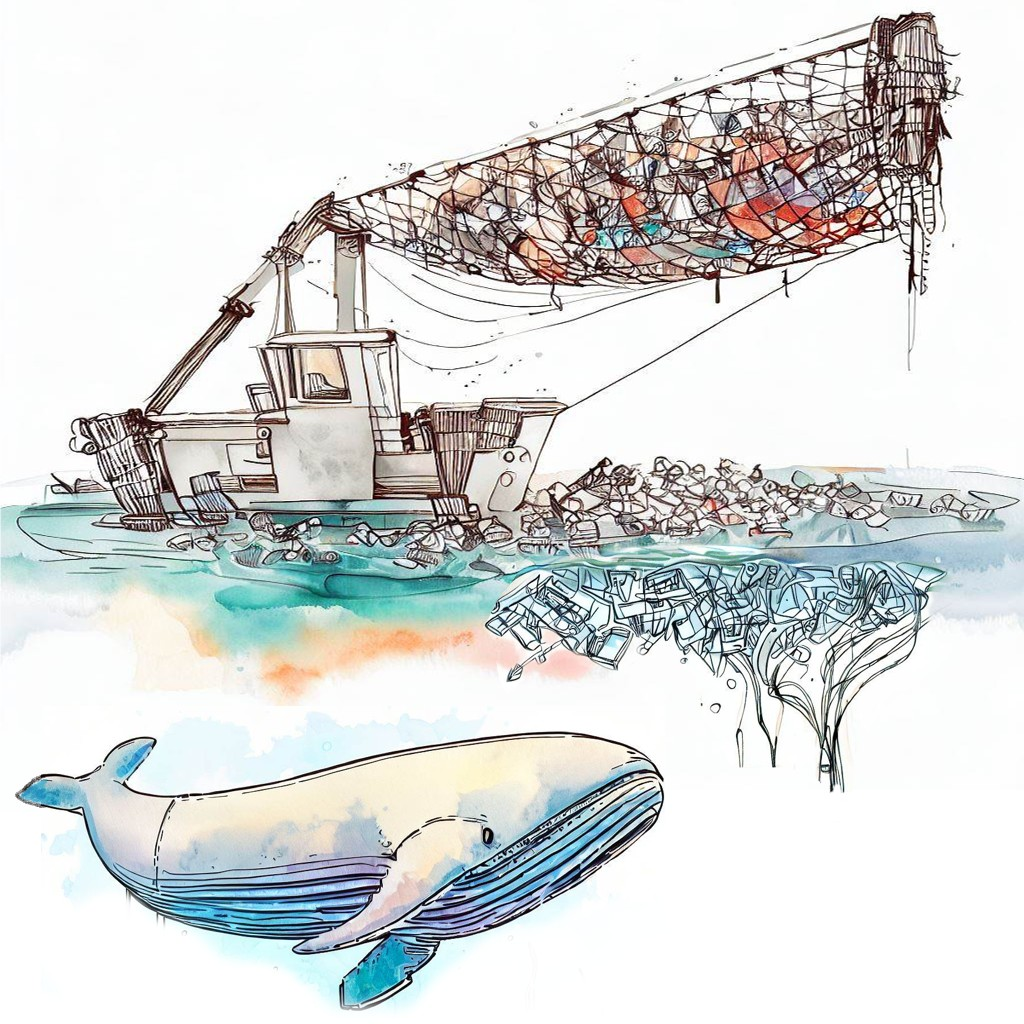
\includegraphics[width=.8\linewidth]{images/ocean-cleanup.jpg}
    \caption{Очищение океана}
  \end{subfigure}
  \caption{Защита природы}
\end{figure}


\newpage
\begin{figure}[h]
  \begin{subfigure}{.5\textwidth}
    \centering
    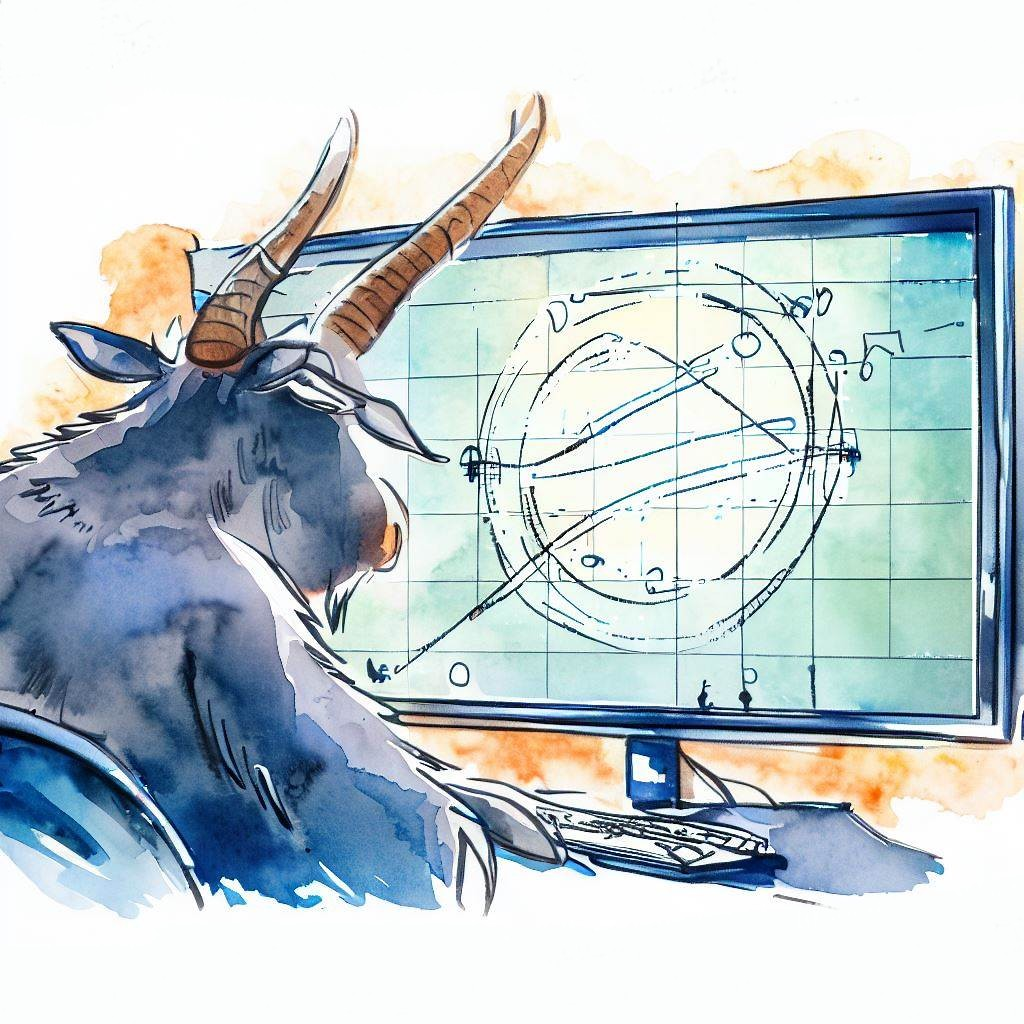
\includegraphics[width=.8\linewidth]{images/gnu-screen.jpg}
    \caption{Расчет траектории зонда}
  \end{subfigure}%
  \begin{subfigure}{.5\textwidth}
    \centering
    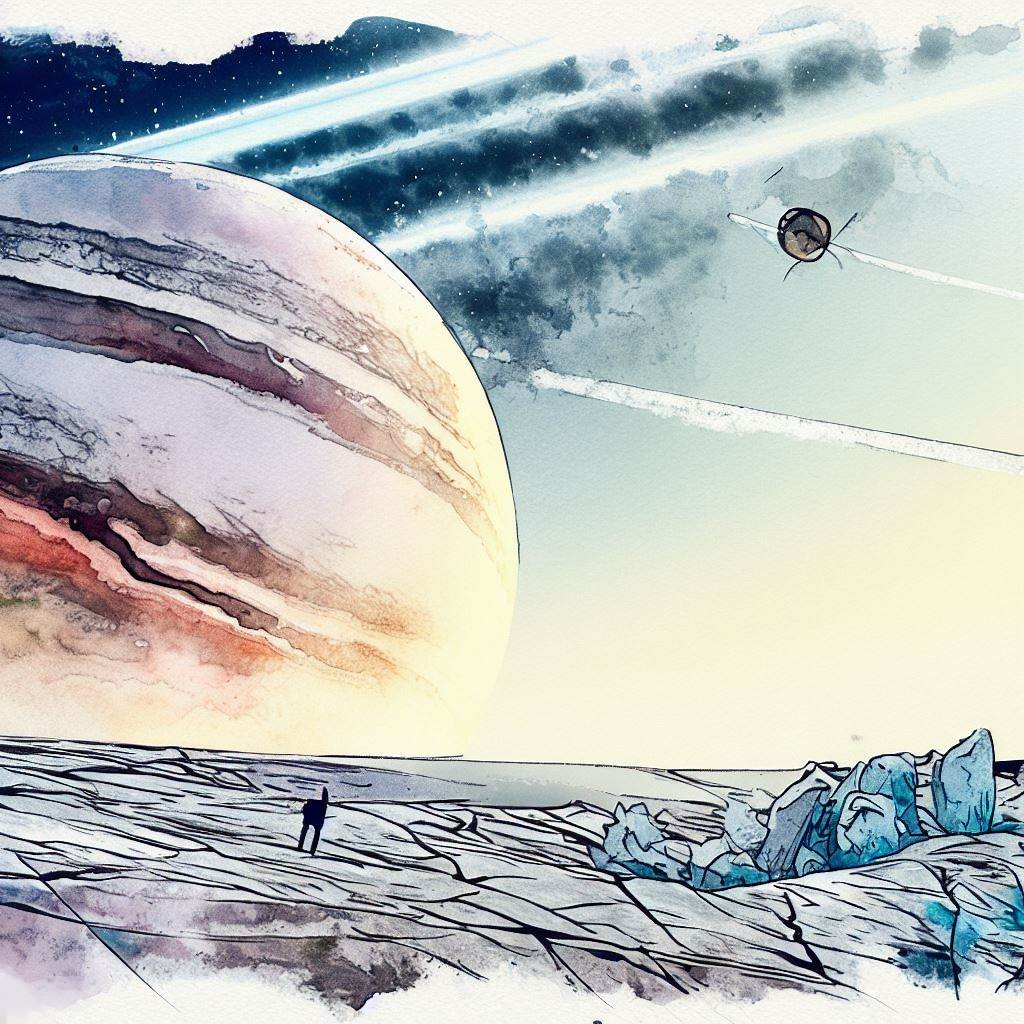
\includegraphics[width=.8\linewidth]{images/europa.jpg}
    \caption{Посадка на Европу}
  \end{subfigure}

  \begin{subfigure}{\textwidth}
    \centering
    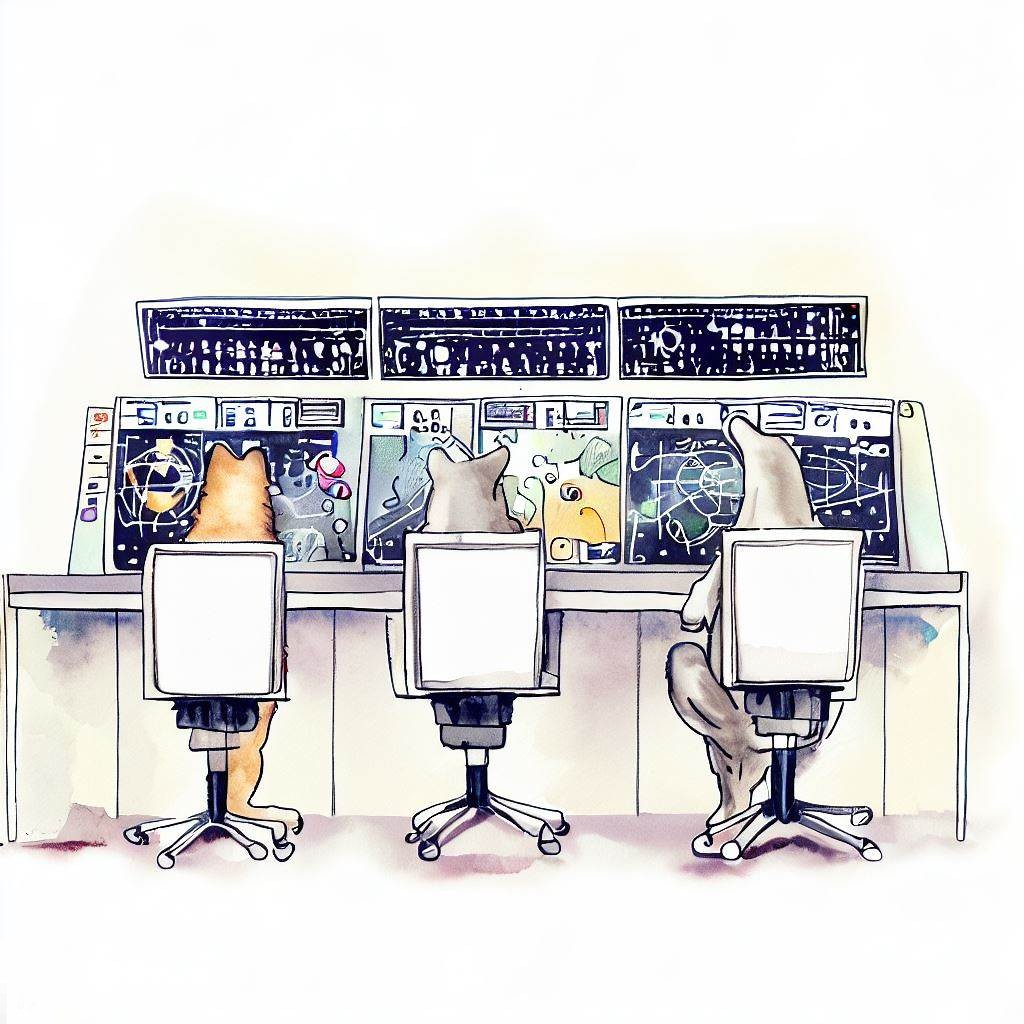
\includegraphics[width=.8\linewidth]{images/control-center.jpg}
    \caption{Центр управления полётами}
  \end{subfigure}
  \caption{Исследование Солнечной системы}
\end{figure}




\restoregeometry

\newpage
\hfill
\backgroundsetup{scale = 1, angle = 0, opacity = 0.9, contents = {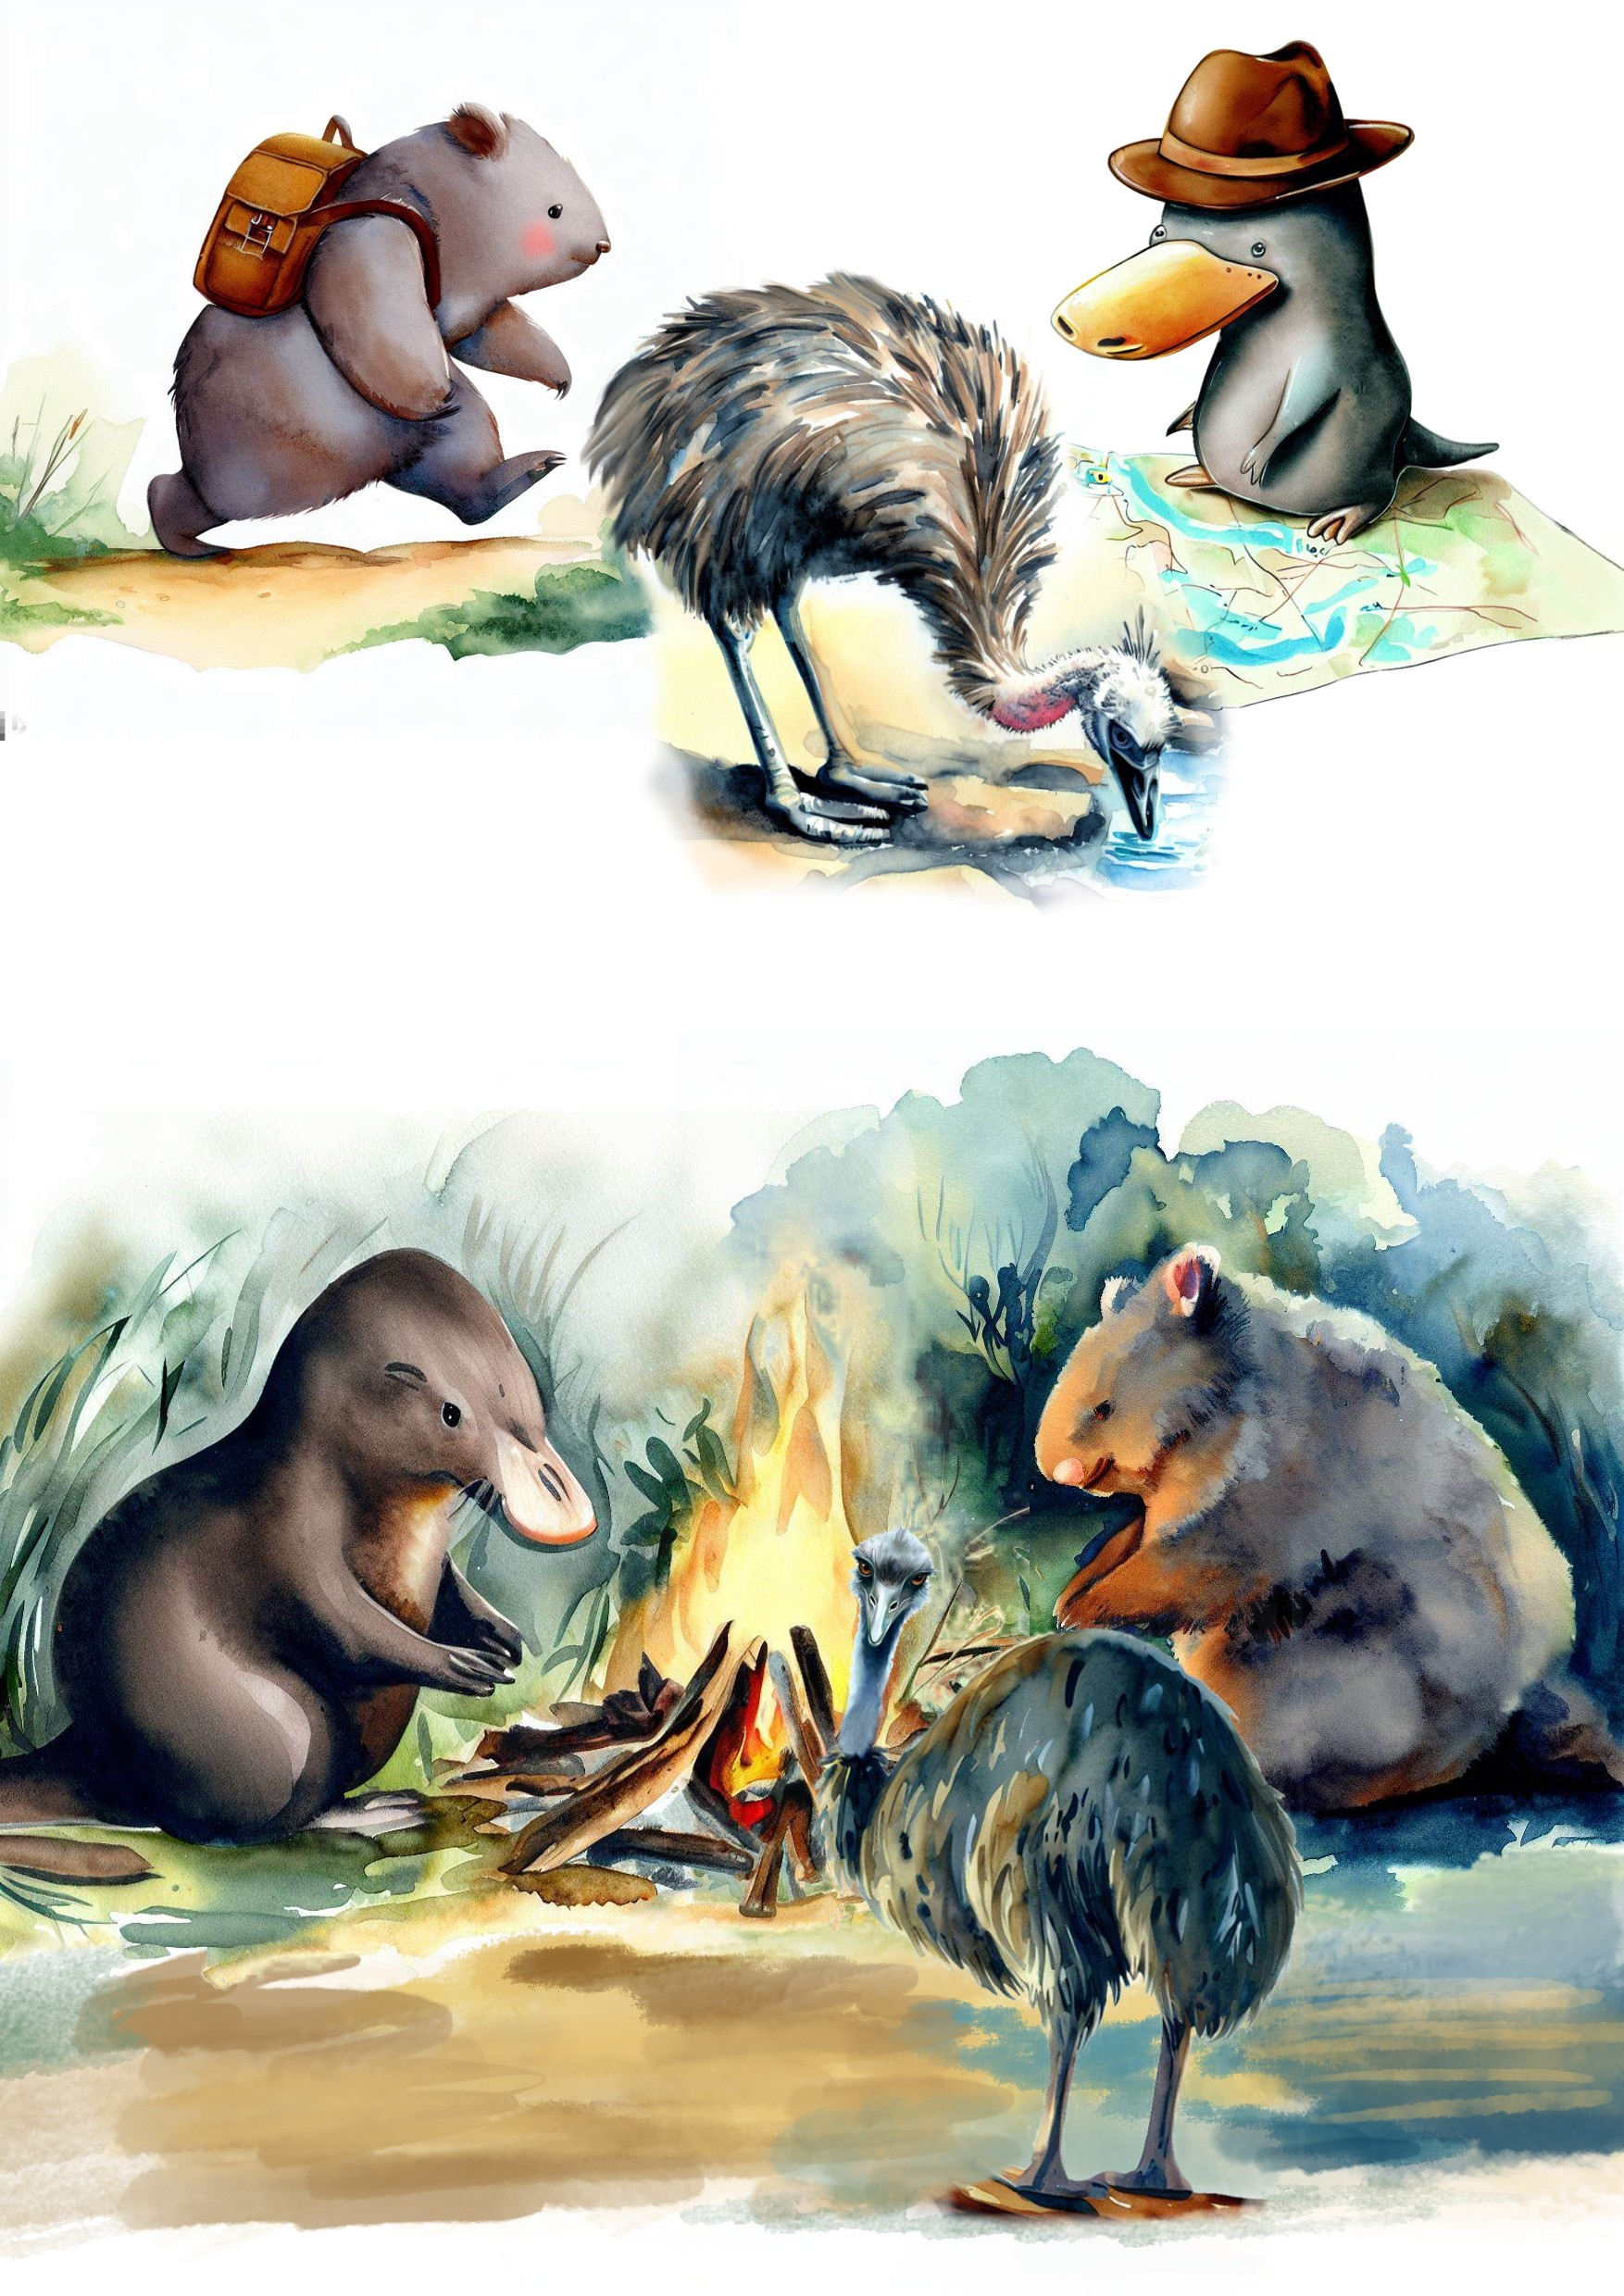
\includegraphics[width = \paperwidth, height = \paperheight] {images/uluru-intro-collage}}}
\BgThispage
\newpage

% night sky star positions correspond to a view from Uluru
\backgroundsetup{scale = 1, angle = 0, opacity = 0.9, contents = {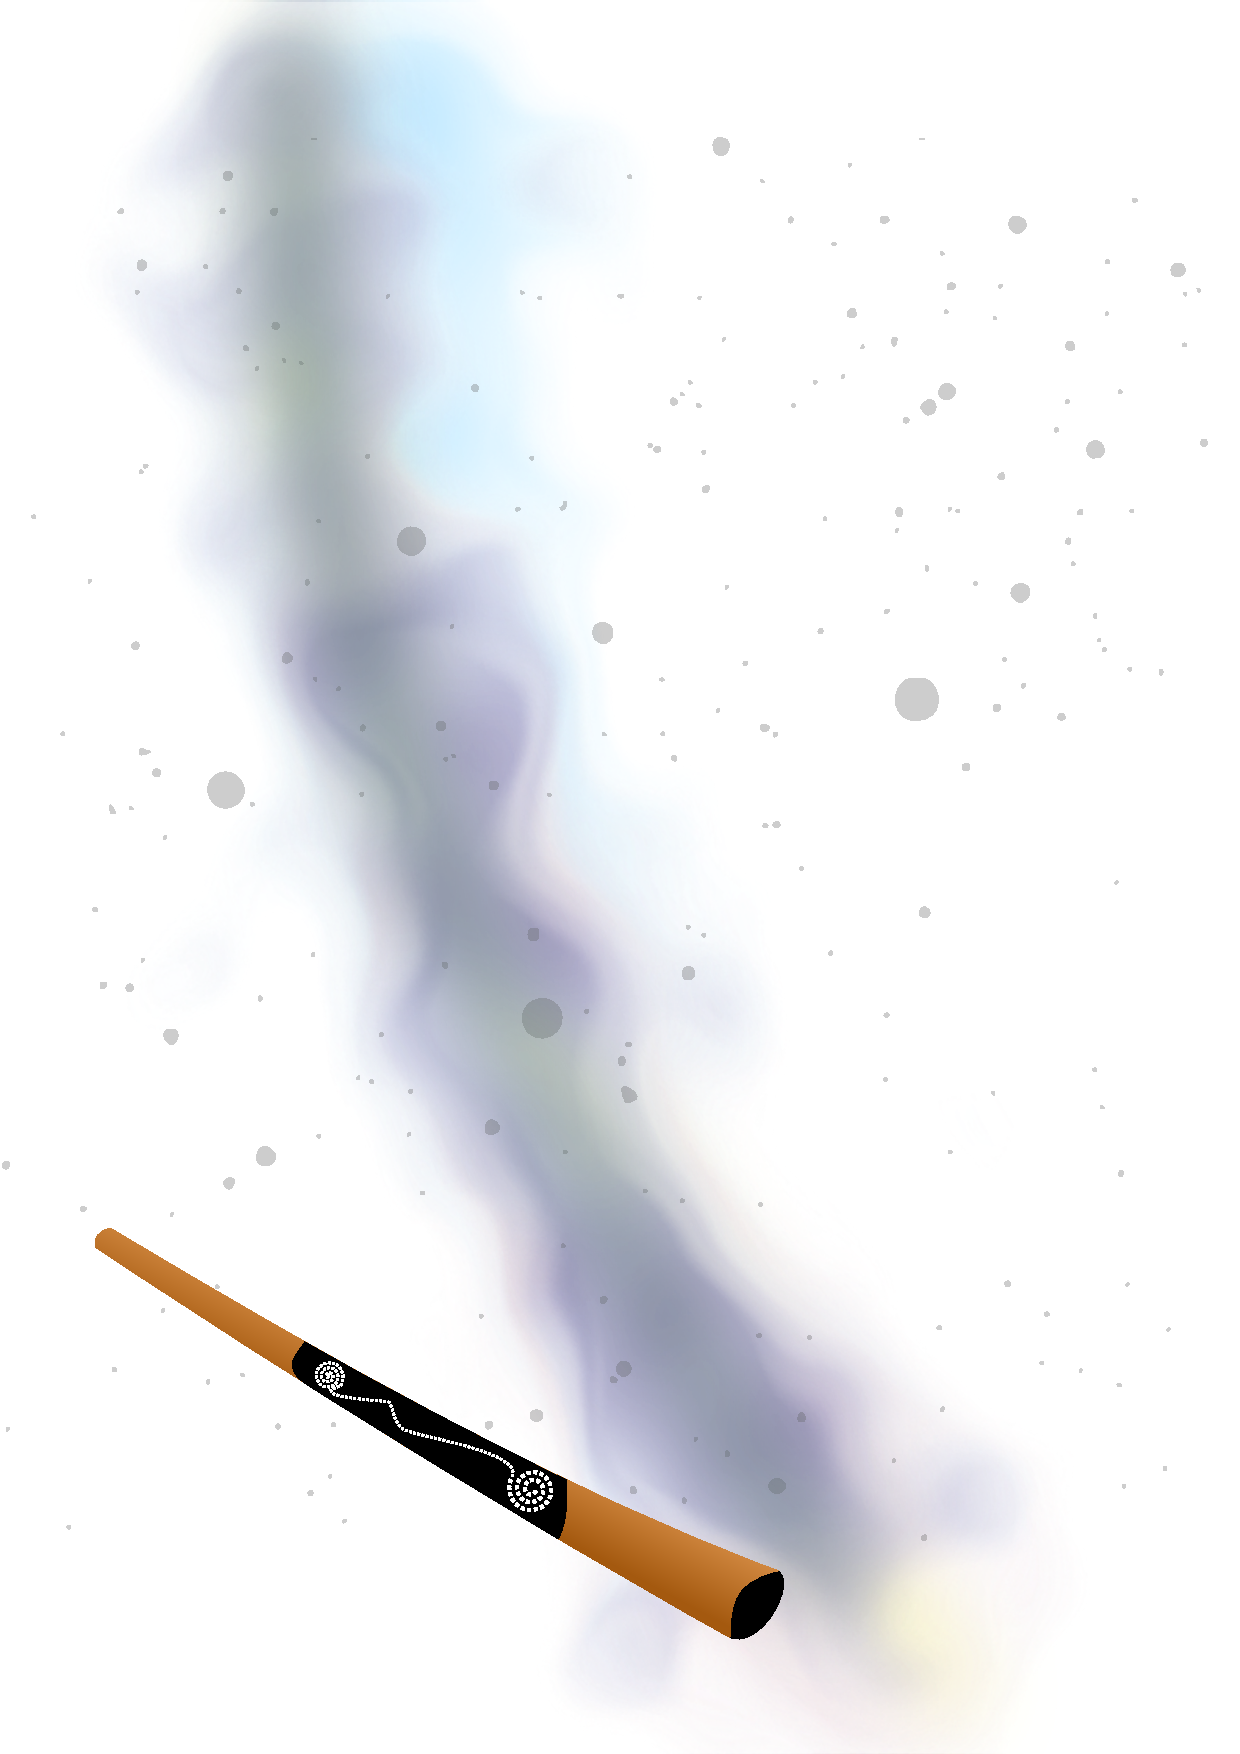
\includegraphics[width = \paperwidth, height = \paperheight] {images/night-sky}}}
\BgThispage

% \renewcommand{\poemtoc}{subsection}
% \PlainPoemTitle
\PoemTitle{Кенгуру у Улур\'{у}}
\settowidth{\versewidth}{Серый кот - господин Мыцумото.}
\begin{verse}[\versewidth]
Как-то раз у горы Улур\'{у}\\
собрались вомб\'{а}т, утконос и эм\'{у}.\\
Уселись они у костра, потеплее\\
и стали разглядывать звезды на небе.
\end{verse}
\label{milky-way}


\begin{verse}[\versewidth]
\hspace{10mm}Одна звезда, две звезды, три, и четыре\ldots\\
\hspace{10mm}зрачки разрастались всё шире и шире,\\
\hspace{10mm}как только их счёт дошёл до пяти\\
\hspace{10mm}их уши услышали чьи-то прыжки.
\end{verse}

\vspace{5mm}
\begin{verse}[\versewidth]
Это их друг --- артист кенгуру,\\
он любит ночами ходить к Улур\'{у}.\\
Приблизившись к свету, увидев вомбата,\\
он крикнул \say{я рад нашей встрече, ребята!\\
Можно я с вами чуть-чуть посижу?}\\
\say{Конечно! Садись!} в хор сказали ему.
\end{verse}

\begin{verse}[\versewidth]
Присев у огня, артист кенгуру\\
Вынул из сумочки диджериду.\\
Вздохнув глубоко, посмотрев на луну,\\
махая хвостом он сказал \say{счас спою!}
\end{verse}

% \vspace{1cm}
% \begin{center}
% 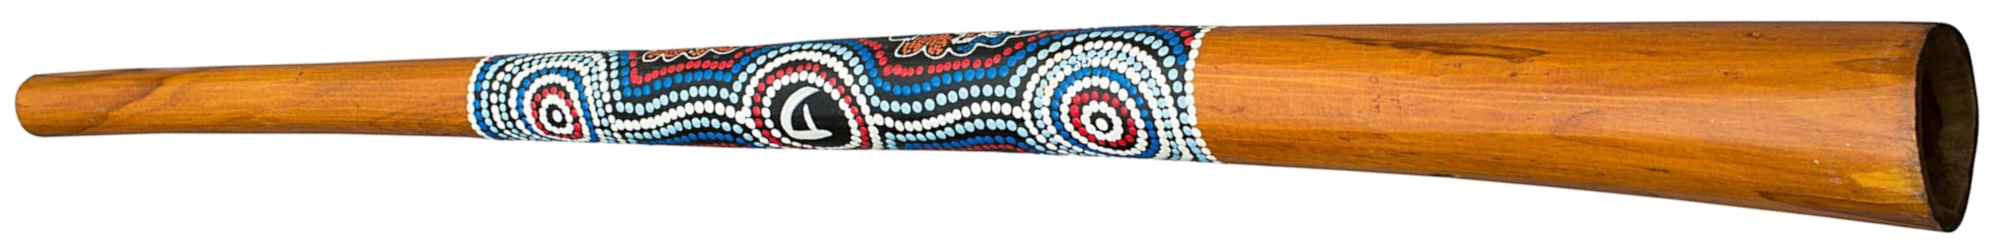
\includegraphics[width=0.6\paperwidth]{images/didgeridoo} 
% \end{center}



\newpage
\hfill

\backgroundsetup{scale = 1, angle = 0, opacity = 0.7, contents = {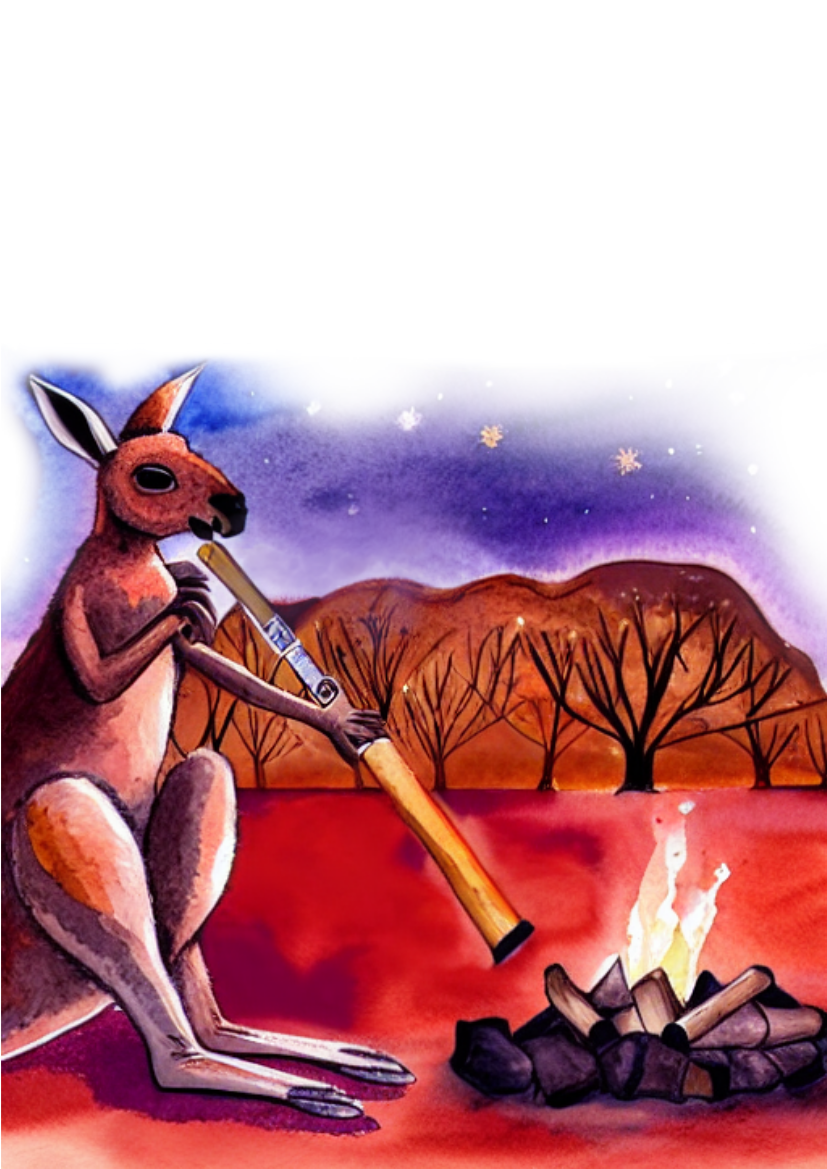
\includegraphics[width = \paperwidth, height = \paperheight] {images/kangaroo-final}}}
\BgThispage
% \newpage


% \fancybreak{* * *}

\begin{verse}[\versewidth]
Вздулись внезапно вокруг паутины\\
гул вырастал в австралийской пустыне.\\
Вууу--{\largeдууу}--{\Largeбууу}--{\LARGEдууу!}\\
Всё громче и громче диджериду!\\
\say{{\LargeВууу}--{\largeдууу}--буу--{\smallдууууу!}}\\
Эхом ответила вслед Улур\'{у}.
\end{verse}
\newpage



\backgroundsetup{scale = 1, angle = 0, opacity = 0.7, contents = {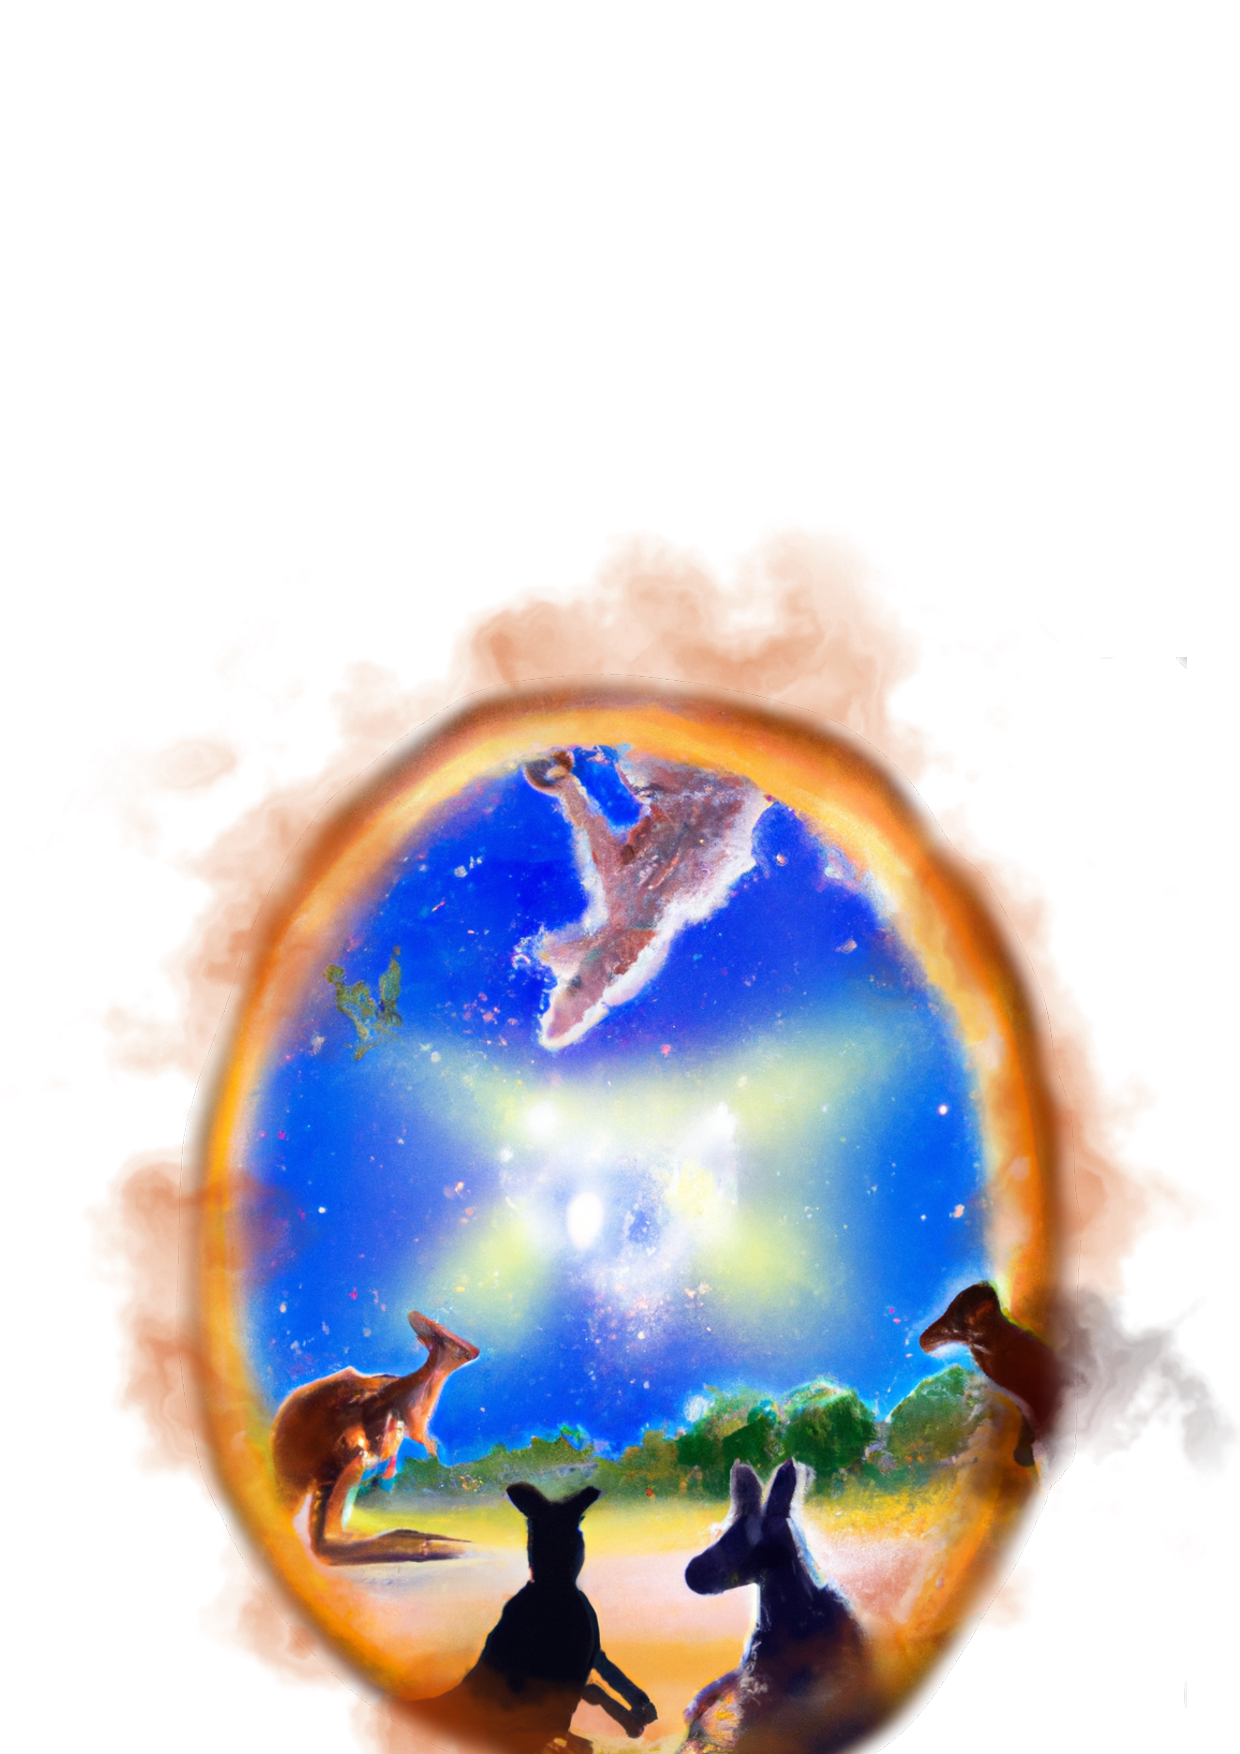
\includegraphics[width = \paperwidth, height = \paperheight] {images/portal}}}
\BgThispage



\begin{verse}[\versewidth]
Такт отбивая правой ногой\\
дверь распахнул кенгуру в мир иной!\\
Звук можно чувствовать клеткой грудной,\\
эм\'{у} кивает в ритм головой.
\end{verse}

% \vspace{4cm}
\begin{verse}[\versewidth]
Все они вдруг от земли оторвались\\
и среди звёзд через миг оказались!\\
Волна их несёт по теченью Пути,\\
ночь разукрасилась, стала цвести!
\end{verse}

\newpage

\begin{verse}[\versewidth]
\hspace{-3cm}Вокруг облака бесконечно, и снова,\\
\hspace{-3cm}точкой становятся, затем и сверхновой.\\
\hspace{-3cm}Время летит то вперёд, то назад,\\
\hspace{-3cm}утконос ничего не может понять!
\end{verse}

\backgroundsetup{scale = 1, angle = 0, opacity = 0.5, contents = {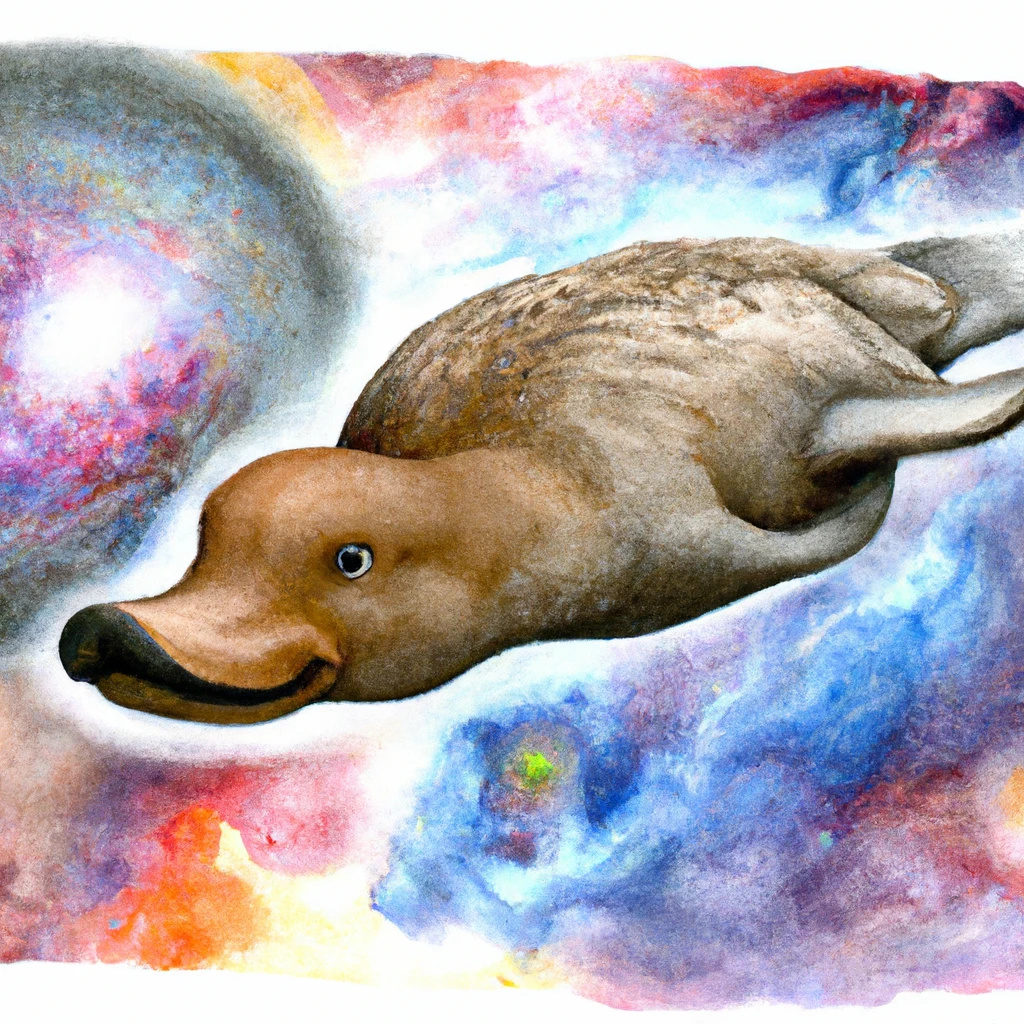
\includegraphics[width = \paperwidth, height = \paperheight] {images/dazed-platypus}}}
\BgThispage

% \begin{center}
% 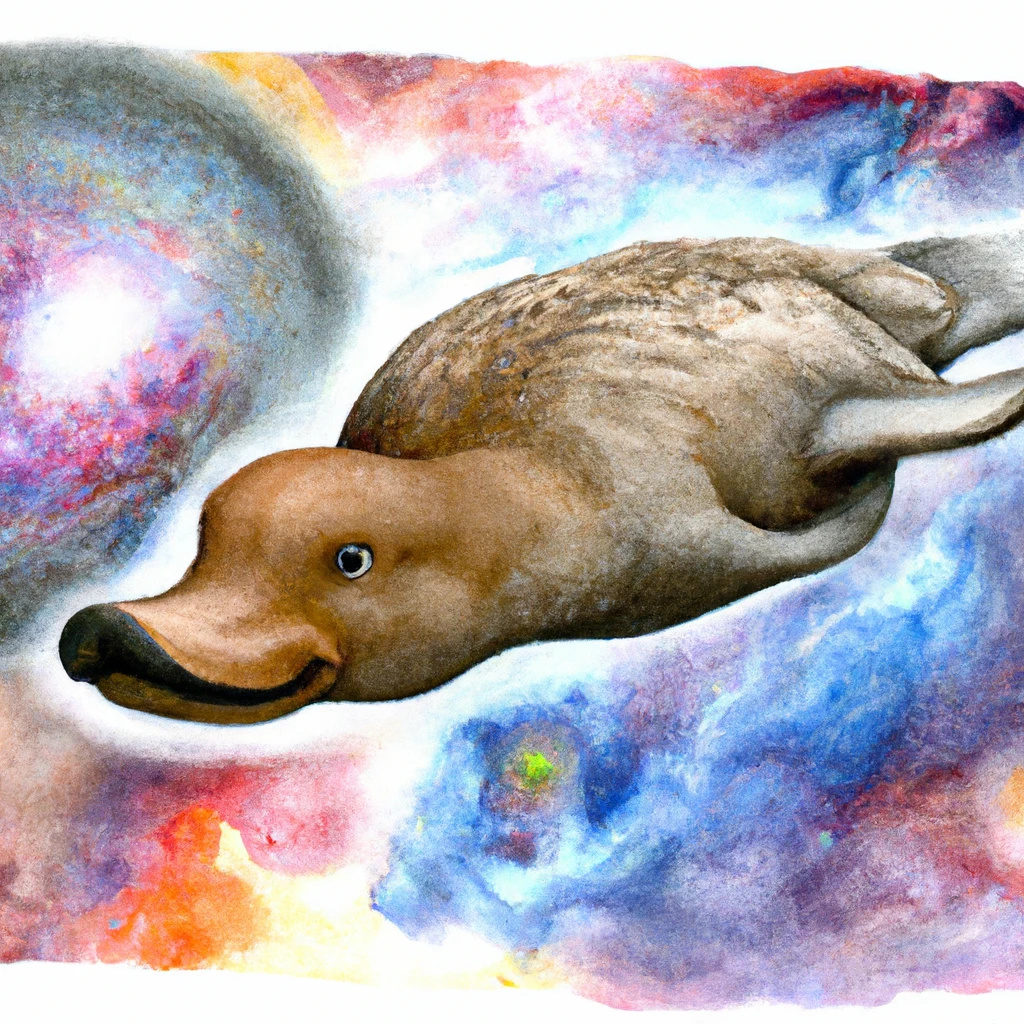
\includegraphics[width=\paperwidth]{images/dazed-platypus.jpg} 
% \end{center}

\vspace{11cm}
\begin{verse}[\versewidth]
\hspace{1cm}Диджериду продолжает гудеть,\\
\hspace{1cm}утконосу от радости хочется петь!\\
\hspace{1cm}Космос раскрылся как цветок на ладони,\\
\hspace{1cm}ритм всё пространство собою заполнил.\\
\hspace{1cm}Нету начала, и нету конца,\\
\hspace{1cm}эта мелодия везде и всегда!
\end{verse}
\newpage

% \fancybreak{* * *}

\begin{verse}[\versewidth]
Солнце вернулось из-за горизонта,\\
гора Улур\'{у} загорелась как охра.\\
Пустыня ожила, и ветер задул,\\
а наш кенгурёнок наконец-то уснул!
\end{verse}

\label{uluru}
\backgroundsetup{scale = 1, angle = 0, opacity = 0.7, contents = {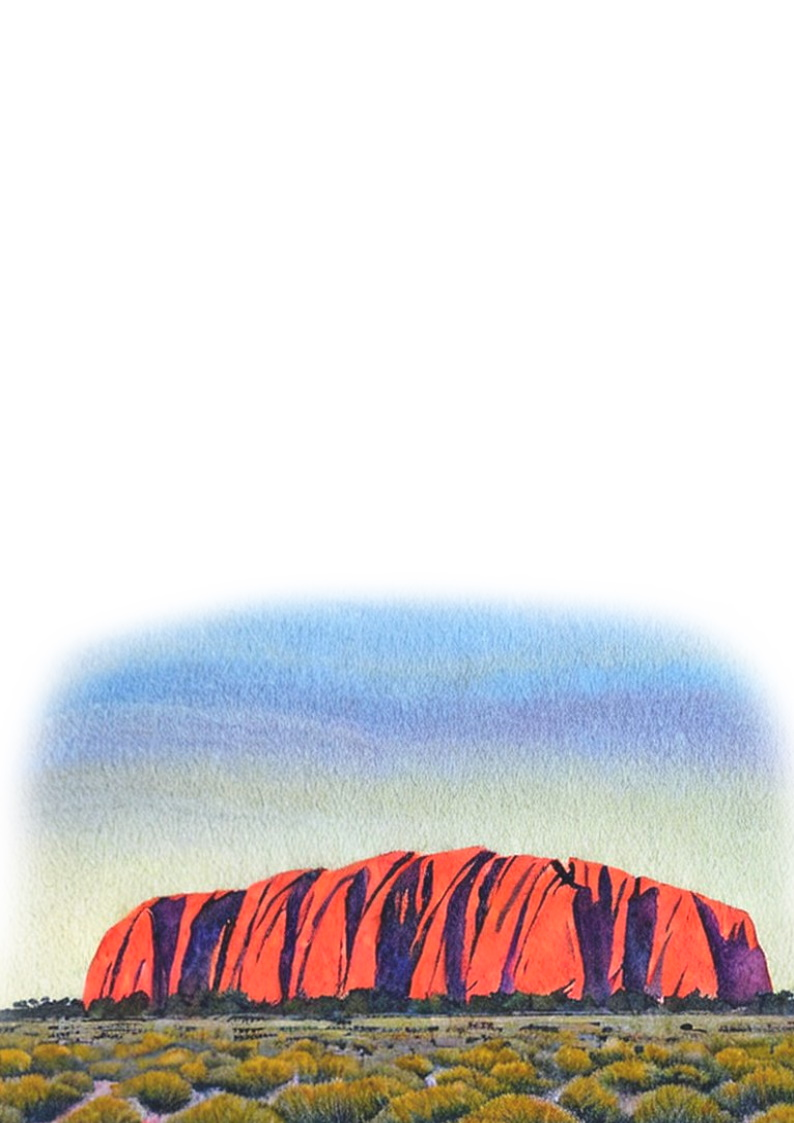
\includegraphics[width = \paperwidth, height = \paperheight] {images/uluru}}}
\BgThispage

\newpage
\hfill
\backgroundsetup{scale = 1, angle = 0, opacity = 1, contents = {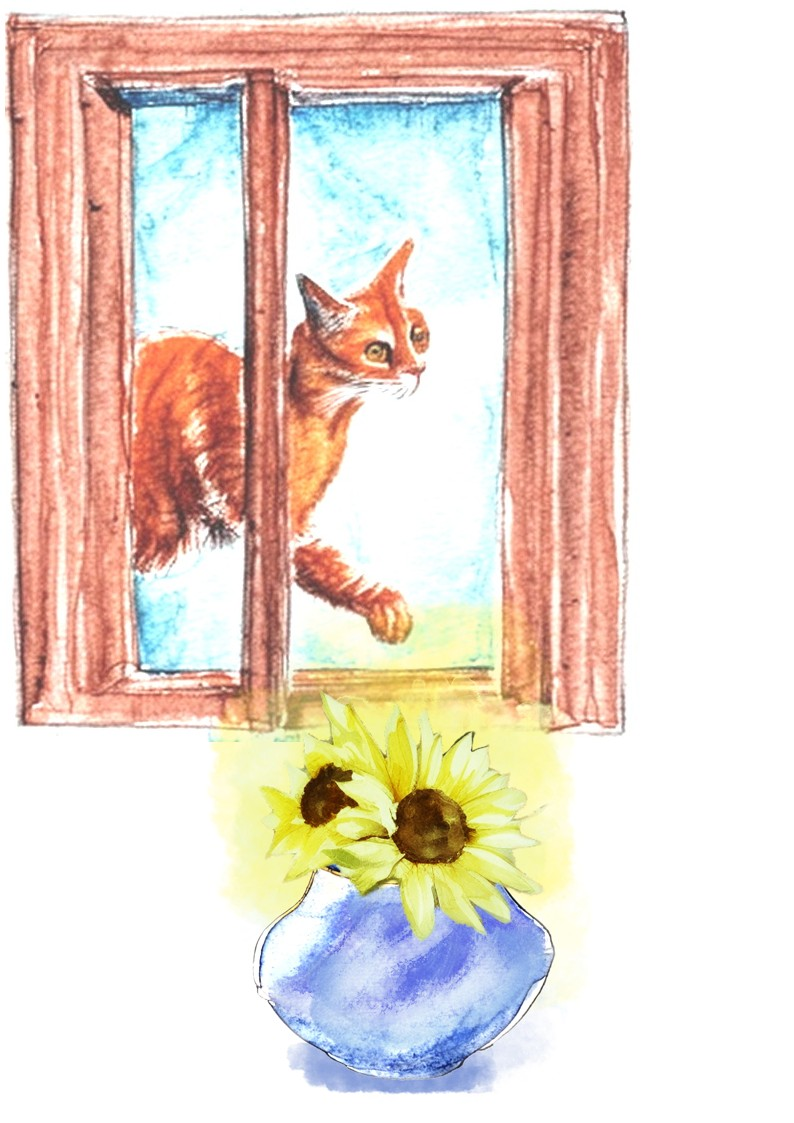
\includegraphics[width = \paperwidth, height = \paperheight] {images/mitsumoto-intro}}}
\BgThispage
\newpage

% \cleartoverso

\PlainPoemTitle
\PoemTitle{Мыцумото из Киото}
% \settowidth{\versewidth}{Серый кот - господин Мыцумото.}
\begin{verse}[\versewidth]
Жил был в префектуре Киото\\
рыжий кот --- господин Мыцумото.\\
Прыгнув однажды в окно, \\
хвостом он задел кимоно. 
\end{verse}

\begin{verse}[\versewidth]
\hspace{-1cm}Шелком шурша\\
\hspace{-1cm}вещь как листик летала,\\
\hspace{-1cm}вазу задела --- ваза упала;\\
\hspace{-1cm}к чашке притронулась ---\\
\hspace{-1cm}чашка разлилась;\\
\hspace{-1cm}лампа на тумбочке\\
\hspace{-1cm}вдруг заискрилась.
\end{verse}

\begin{verse}[\versewidth]
\hspace{-2cm}Ваза разбилась,\\
\hspace{-2cm}разлетелись кусочки, \\
\hspace{-2cm}на полу оказались \\
\hspace{-2cm}из вазы цветочки. \\
\end{verse}

\backgroundsetup{scale = 1, angle = 0, opacity = 1, contents = {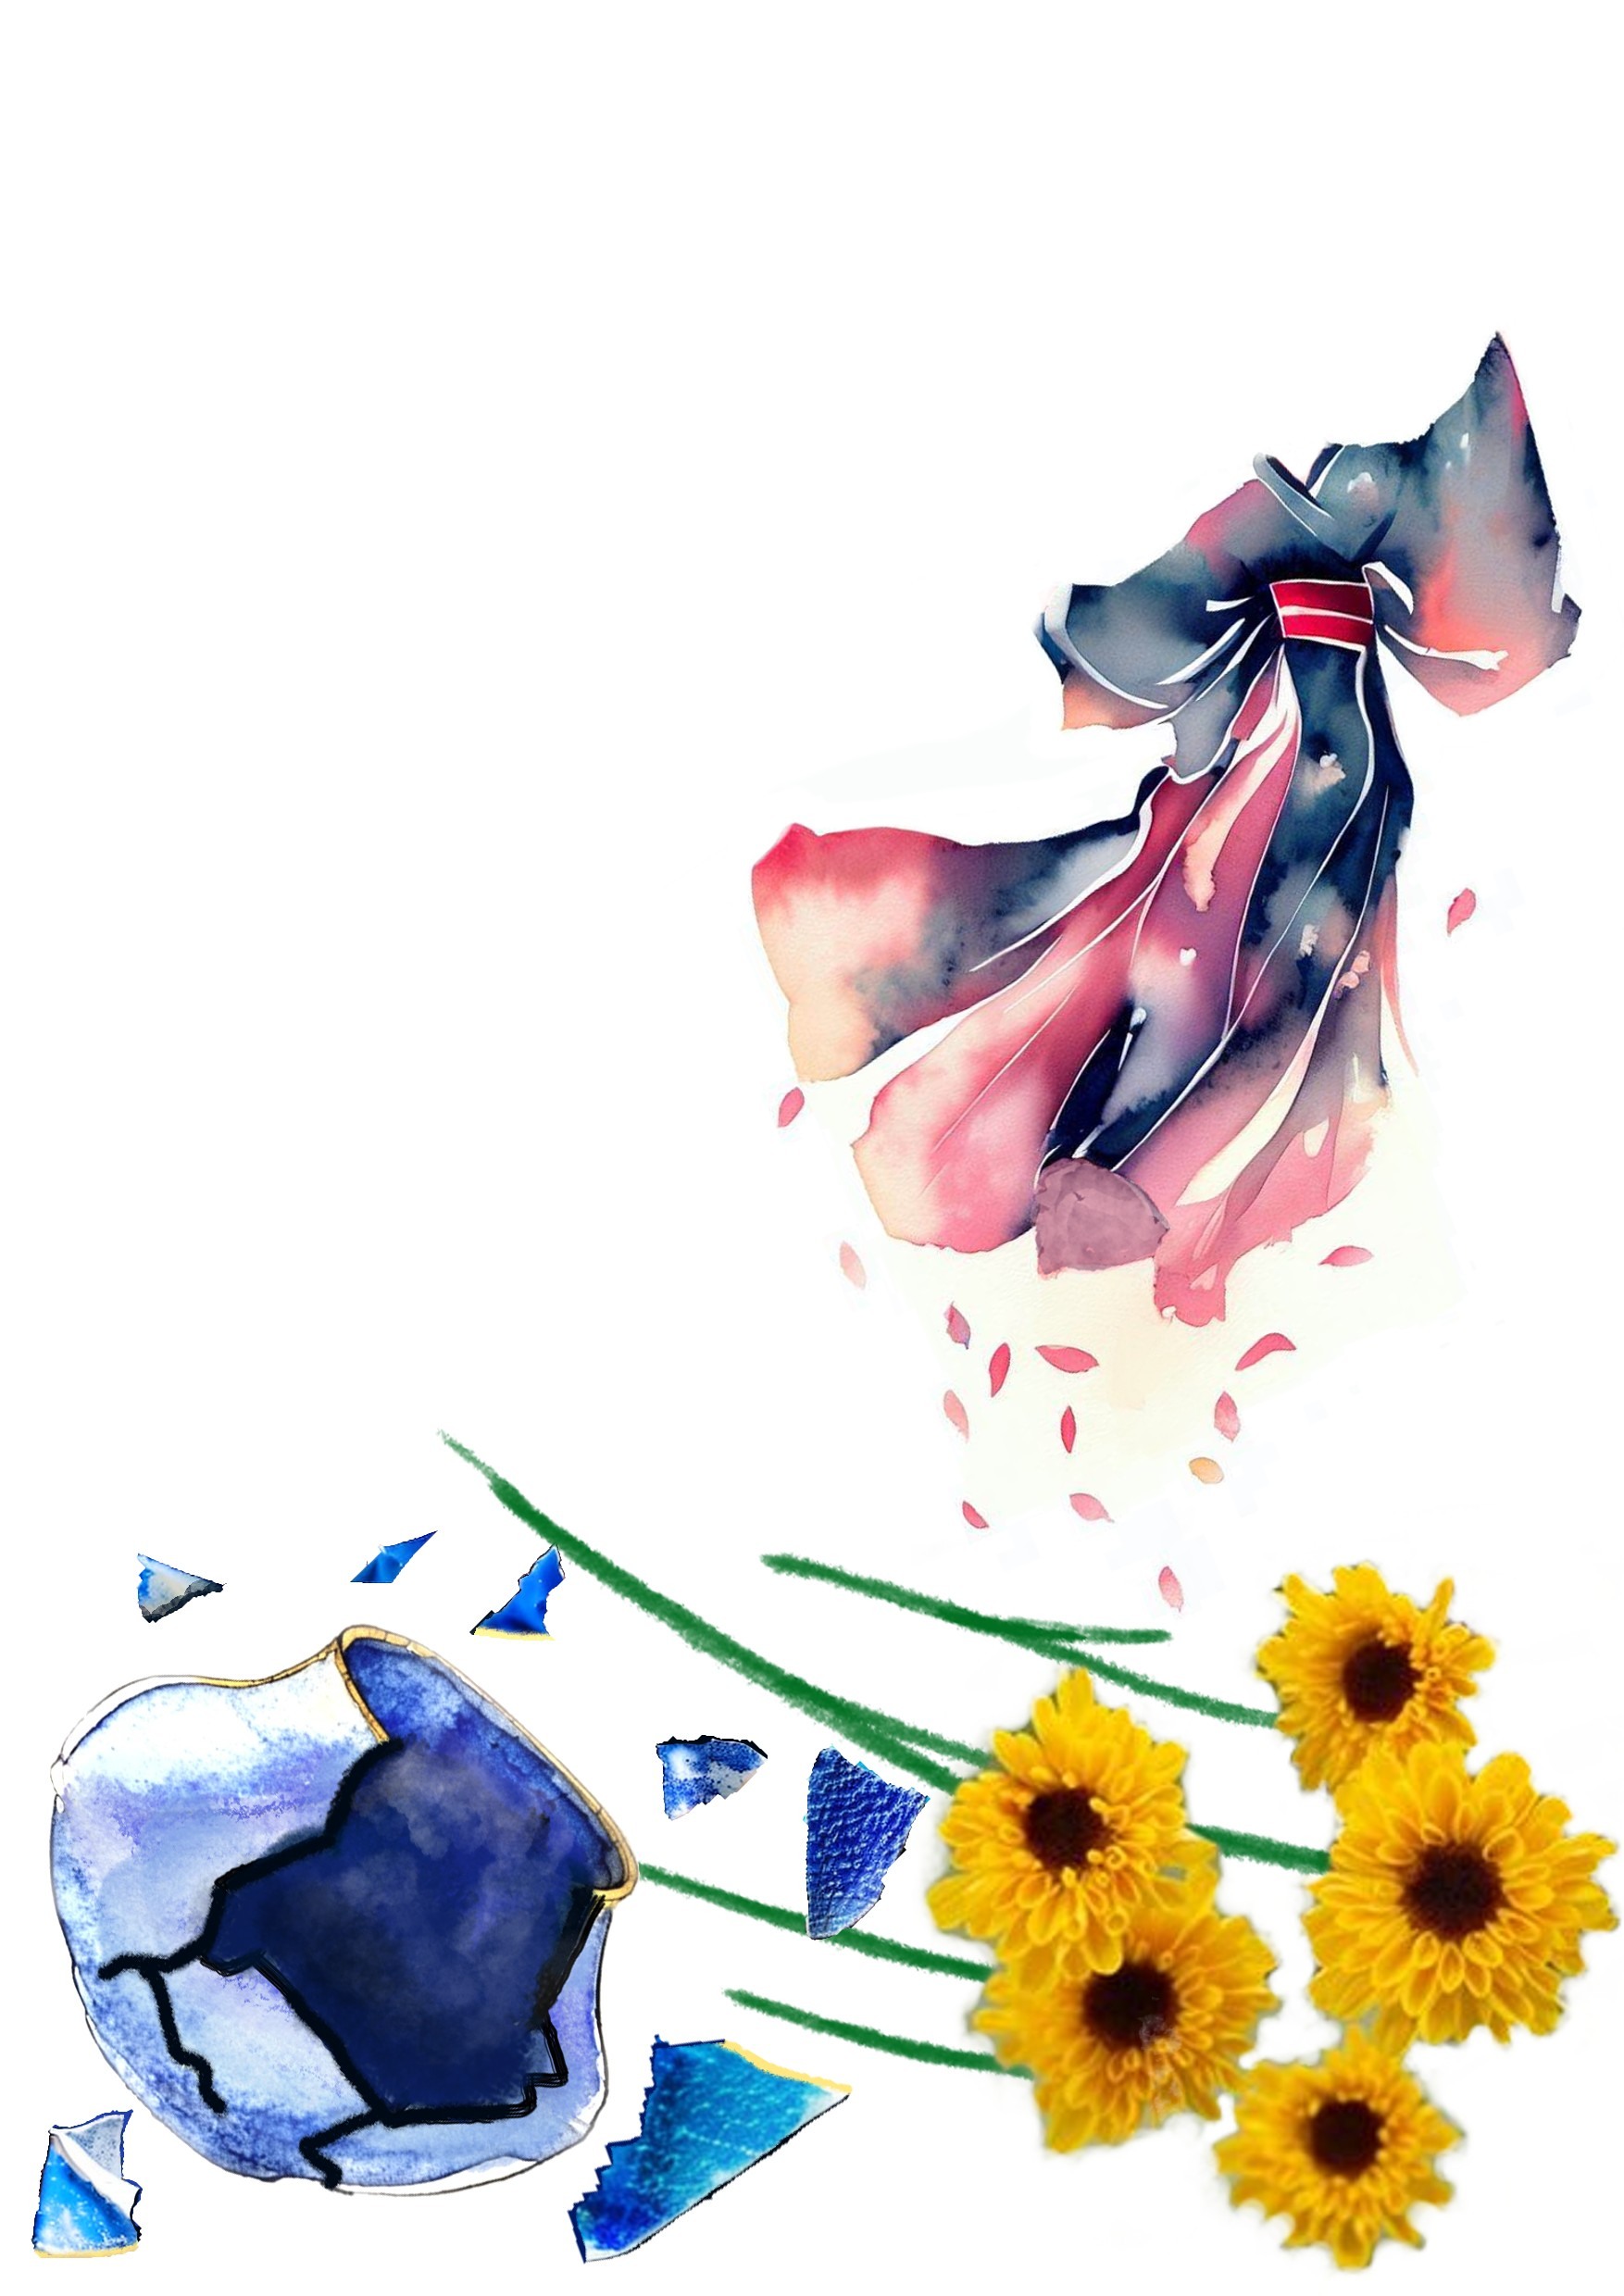
\includegraphics[width = \paperwidth, height = \paperheight] {images/collage-kimono-broken-vase}}}
\BgThispage


\clearpage
\backgroundsetup{scale = 1, angle = 0, opacity = 1, contents = {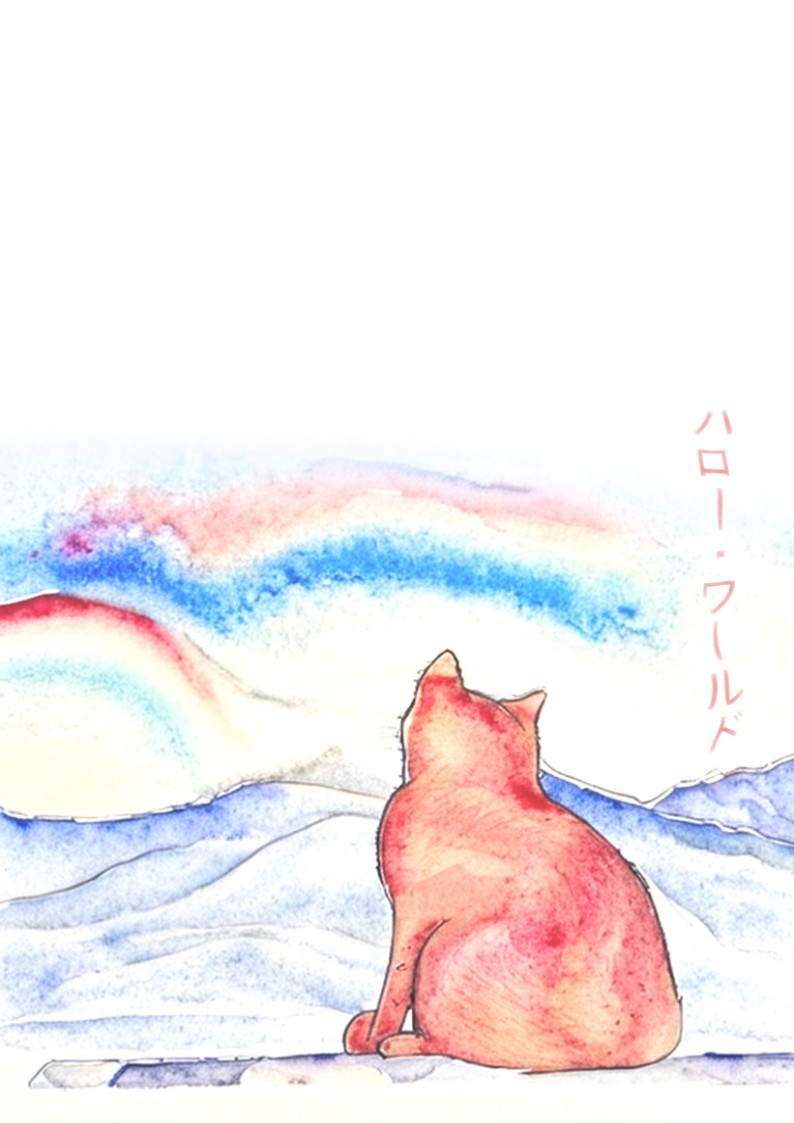
\includegraphics[width = \paperwidth, height = \paperheight] {images/mitsumoto-hello-world-sunrise}}}
\BgThispage

% \fancybreak{* * *}

\begin{verse}[\versewidth]
На шерсти почувствовав солнца лучи \\
смотрел Мыцумото на горы вдали. \\
\say{Ах, как прекрасно день начался! \\
Так приятно купаться в рассвета лучах!}
\end{verse}

\begin{verse}[\versewidth]
В небесах облака словно множество линий \\
градиент переходит из красного в синий, \\
птицы запели, раскрылись цветы, \\
не осталось ни следа от темноты. 
\end{verse}

% EXPERIMENT: put a semi-transparent white rectangle underneath, for contrast
% \begin{verse}[\versewidth]
% \hspace{-1.8mm}\tikz \node[text width=10cm, fill=white, fill opacity=0.7, text opacity=1]{
% На коврике сидя, господин Мыцумото\\ 
% забыл о работе, забыл о заботах\ldots \\
% он слился с природой, \\
% растворил в ней свой ум,\\ 
% всё вдруг затихло, исчез всякий шум\ldots
% };
% \end{verse}


% \begin{verse}[\versewidth]
% На коврике сидя, господин Мыцумото\\ 
% забыл о работе, забыл о заботах\ldots \\
% он слился с природой, \\
% растворил в ней свой ум,\\ 
% всё вдруг затихло, исчез всякий шум\ldots
% \end{verse}

% \hspace{-3cm}
\begin{verse}
\vspace{-5mm}\hspace{7mm} % compensate space added by bounding rectangle
\tikz \node[text width=10cm, fill=white, 
    path fading = side shaded,
    text opacity=1, inner xsep=2cm, inner ysep=0.5cm]{
На коврике сидя, господин Мыцумото\\ 
забыл о работе, забыл о заботах\ldots \\
он слился с природой, \\
растворил в ней свой ум,\\ 
всё вдруг затихло, исчез всякий шум\ldots
};
\end{verse}


% EXPERIMENT of writing white text on a blurred background
% \begin{verse}[\versewidth]
% \hspace{-3mm}\begin{tikzpicture}
% \blurry{На коврике сидя, господин Мыцумото}{white}
% \end{tikzpicture}
% забыл о работе, забыл о заботах\ldots \\
% он слился с природой, \\
% растворил в ней свой ум,\\ 
% всё вдруг затихло, исчез всякий шум\ldots
% \end{verse}



\clearpage
% \fancybreak{* * *}

\begin{verse}[\versewidth]
Вернувшись обратно, запрыгнув в окно, \\
Мыцумото заметил что что-то не то. \\
Он тихо поднял и сложил кимоно. 
\end{verse}

\begin{verse}[\versewidth]
Он лапой собрал на полу лепесточки, \\
временно в банку поставил цветочки,\\ 
лампу протёр, починил выключатель, \\
чашку поднял, промяукав \say{что дальше?}
\end{verse}

\begin{verse}[\versewidth]
А дальше он вазы нашёл все кусочки \\
и клей-порошок он достал из мешочка,\\
собрал воедино, как пазл осколки, \\
уж очень любил он\ldots ~головоломки!
\end{verse}


\backgroundsetup{scale = 1, angle = 0, opacity = 1, contents = {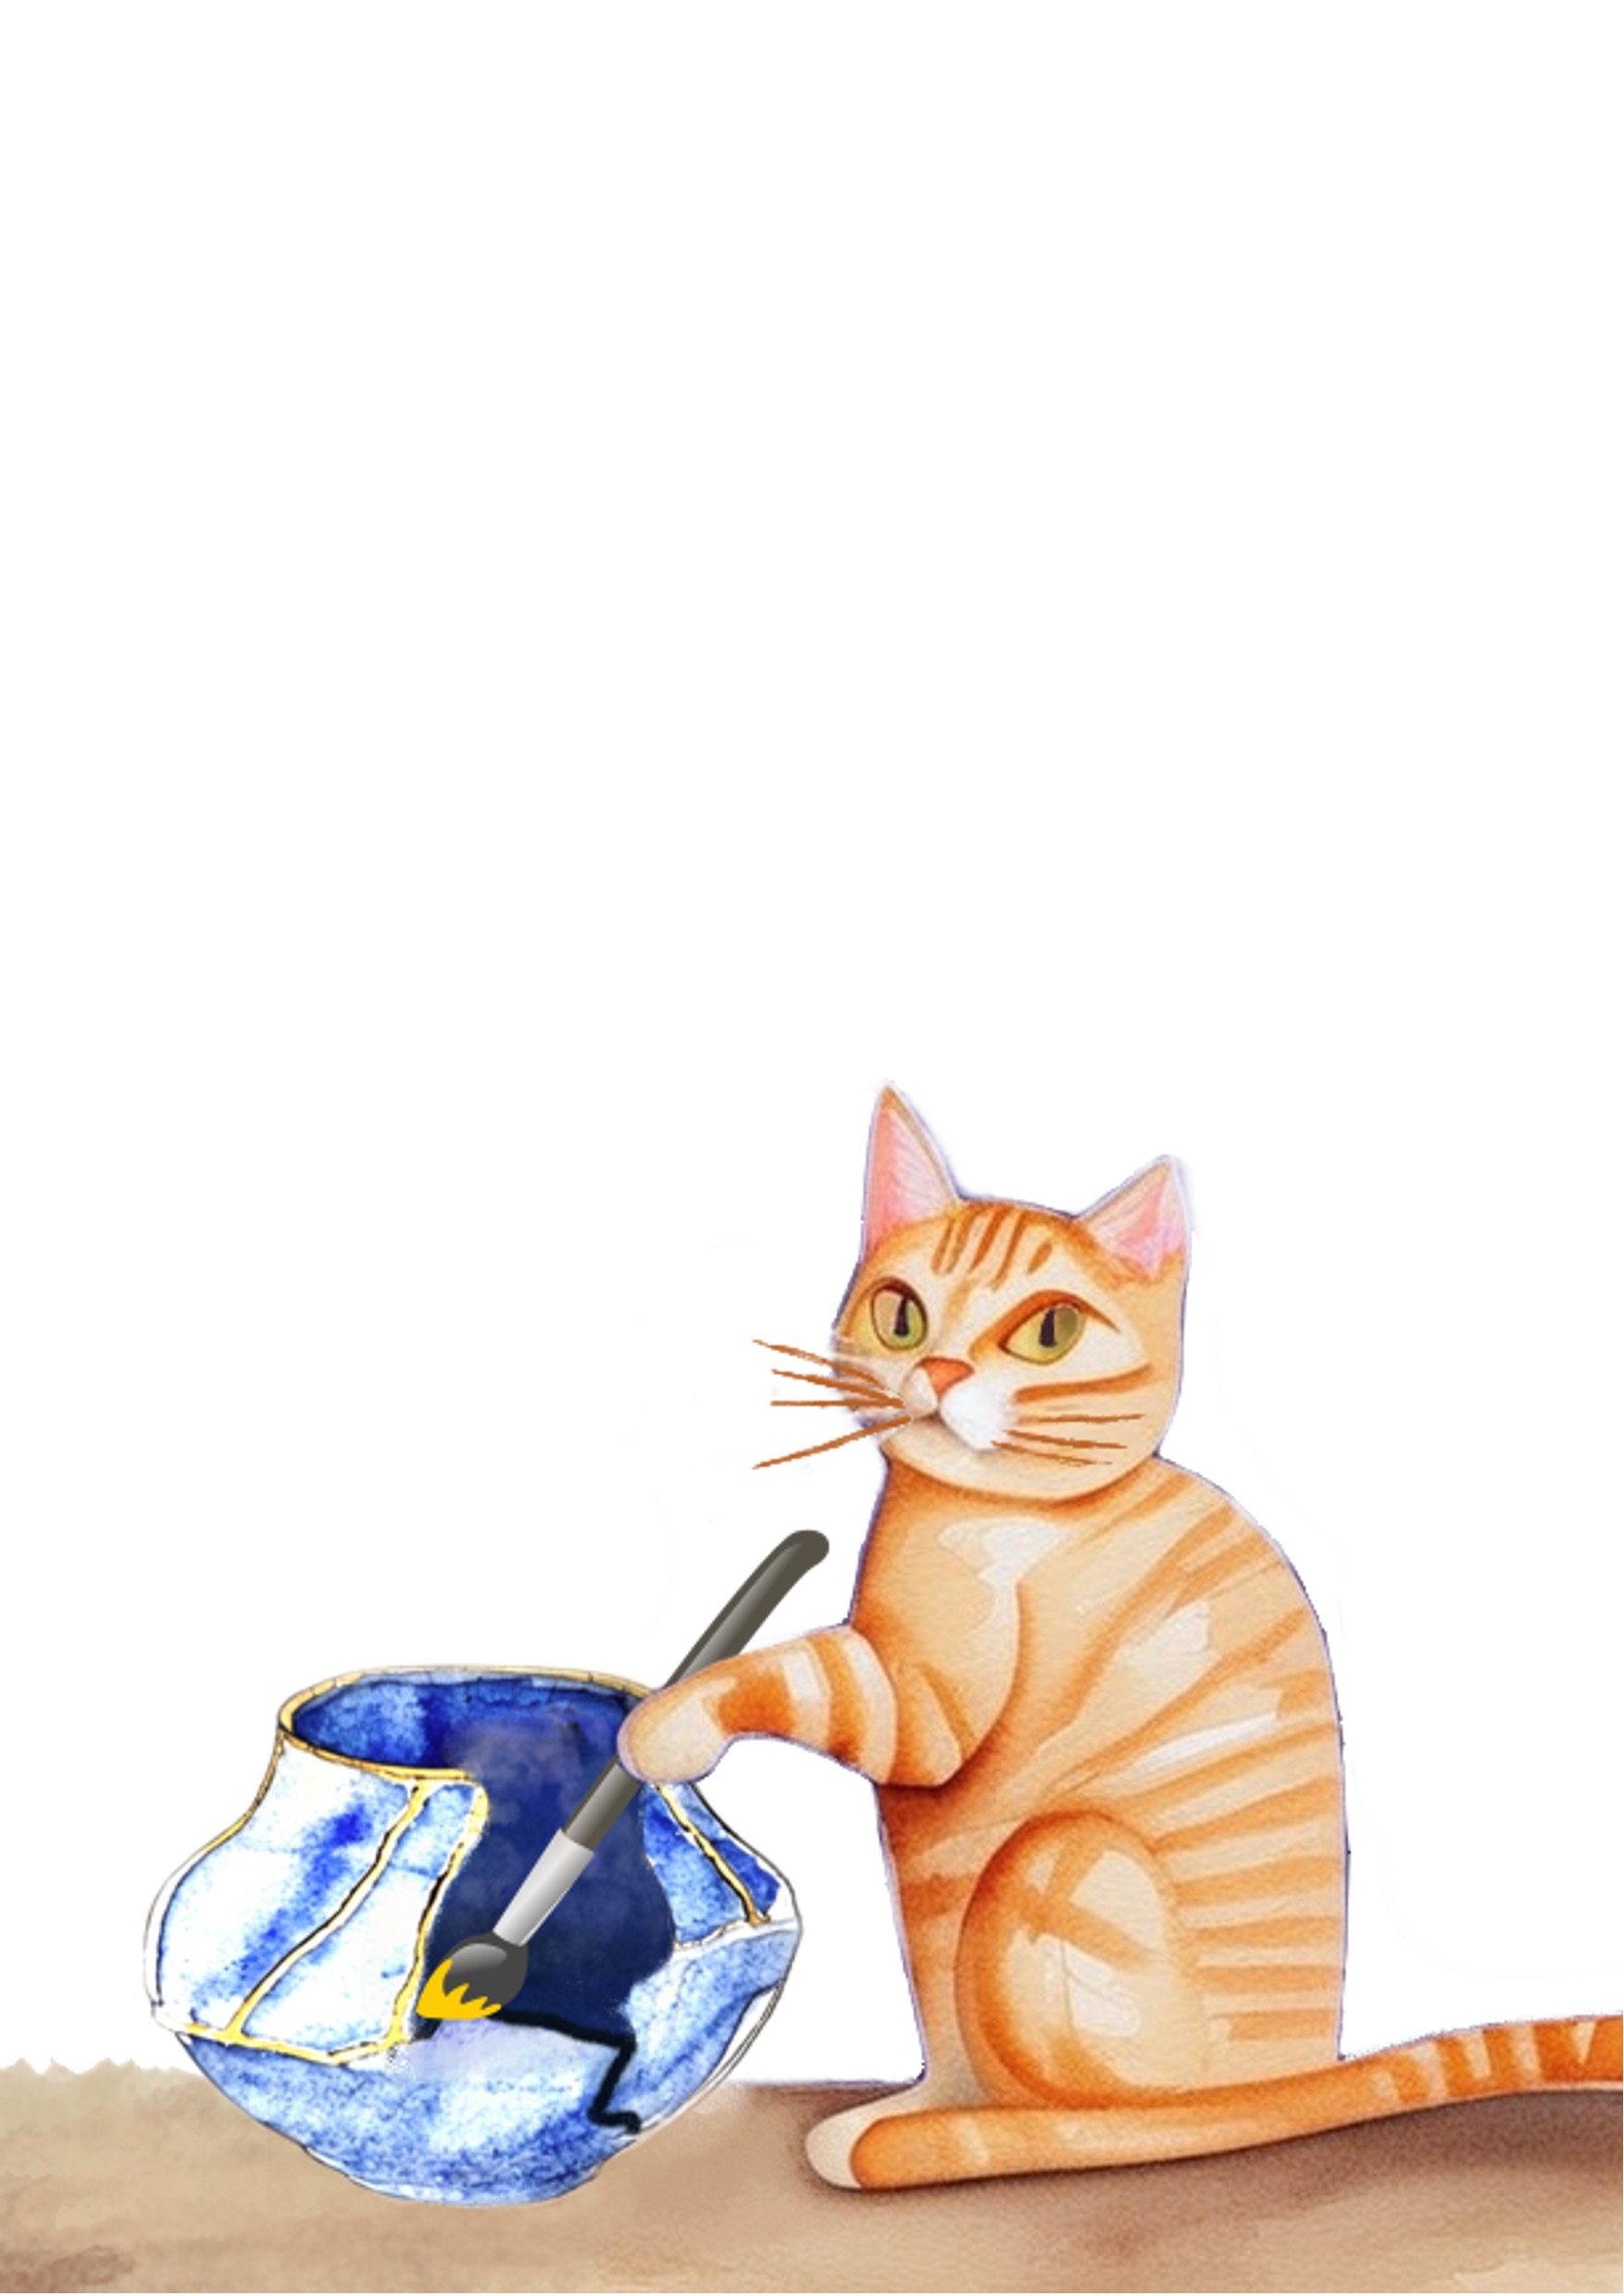
\includegraphics[width = \paperwidth] {images/cat-fix-vase-a5}}}
\BgThispage

\newpage

\begin{verse}[\versewidth]
Трещины кисточка лаком ласкает, \\
керамику в жизненный путь возвращает. \\
на прежнее место цветочки вернулись\\ 
и к солнцу опять лепестки повернулись.
\end{verse}

\begin{verse}[\versewidth]
Стала теперь наша ваза сильнее, \\
господин Мыцумото --- стал чуть мудрее.
\end{verse}

\vspace{1cm}

\begin{center}
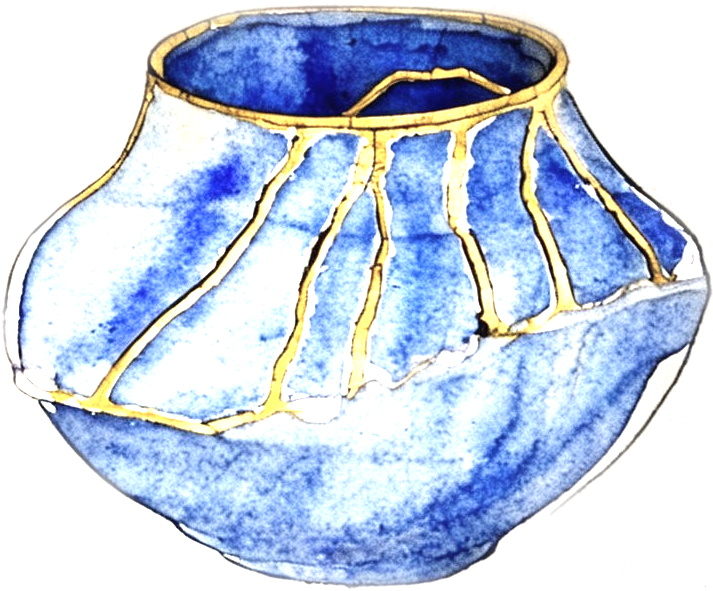
\includegraphics[height=8cm]{images/vase} 
\end{center}
\newpage

\vspace{-2cm}
\begin{center}
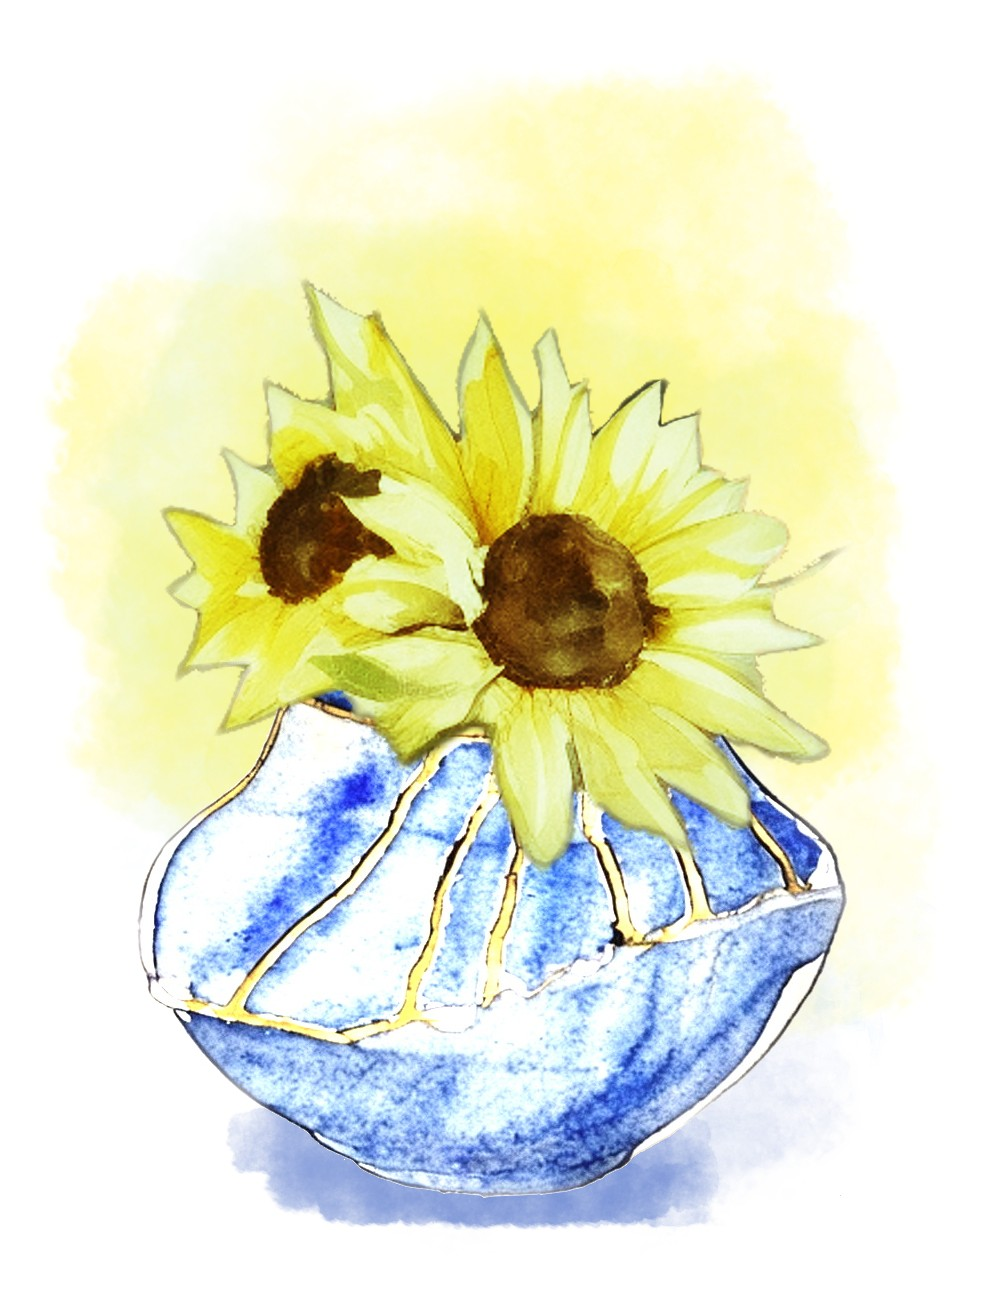
\includegraphics[height=8cm]{images/vase-flowers-repaired} 
\end{center}

\begin{center}
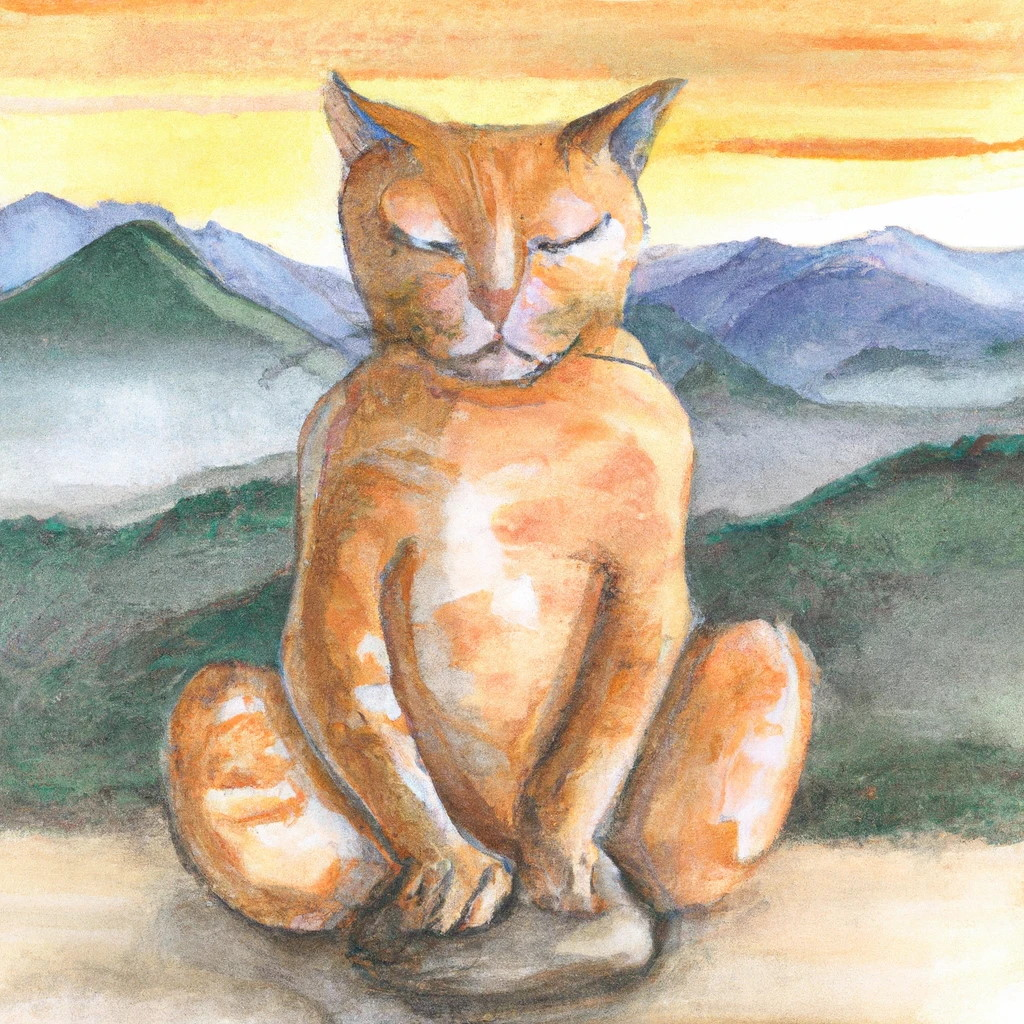
\includegraphics[height=8cm]{images/mitsumoto-front.jpg} 
\end{center}

\newpage




\PlainPoemTitle
\PoemTitle{Удача и неудача}
\vspace{-4mm}
\begin{center}\small{\textit{(по мотивам китайской сказки)}}\end{center}

\begin{verse}[\versewidth]
Жил-был в провинции Хубэй \\
да на ферме усердно работал, \\
Лао Вэнг ---  любимец детей, \\
с тремя сыновьями и дочкой. \\
\end{verse}

\begin{verse}[\versewidth]
Была у них лошадь с белою гривой, \\
была она умной, доброй, игривой\ldots \\
Любила лошадка по ферме скакать, \\
воду носить, да тележку таскать. \\
\end{verse}

\begin{verse}[\versewidth]
Утром, однажды, заметили все ---  \\
что стойло пустует, и лошади нет! \\
Засуетились люди в селе ---  \\
лошадь искали, искали везде\ldots \\
За холмами, в лесу, и вниз по реке\ldots \\
Но след от лошадки не найден нигде. \\
\end{verse}

\begin{verse}[\versewidth]
И сказали тогда все в селе: \\
\say{Вот горе! Вот невезенье! \\
Ах, великая беда! \\
Не повезло старине Лао Вэнгу, \\
ох и тяжелая эта судьба\ldots} \\
\end{verse}

\begin{verse}[\versewidth]
Лао подумал, дал печали остыть, \\
помолчал, и сказал \say{может быть\ldots} \\
\end{verse}

\begin{verse}[\versewidth]
Прошел день. \\
Прошло два. \\
Ночь накрыла село. \\
На небо явилась луна. \\
\end{verse}

\begin{verse}[\versewidth]
Всех разбудил шум копыт! \\
Неужели наступает орда?!?! \\
\end{verse}

\begin{verse}[\versewidth]
Это лошадка вернулась в село, \\
но вернулась она не одна! \\
Семь лошадей привела за собой: \\
шесть кобыл и коня! \\
\end{verse}

\begin{verse}[\versewidth]
Дикие звери, здоровые звери, \\
гривы как из серебра! \\
К Лао на ферму как ветер примчались, \\
и машут хвостами то туда, то сюда\ldots \\
\end{verse}

\begin{verse}[\versewidth]
\say{Вот повезло! Вот это удача! \\
Ну и везёт же тебе, старина! \\
Получил ты от жизни огромный подарок, \\
ах, вот это судьба!} \\
\end{verse}

\begin{verse}[\versewidth]
Лао подумал, дал веселью остыть, \\
помолчал, и сказал \say{может быть\ldots} \\
\end{verse}

\begin{verse}[\versewidth]
День спустя, все решили --- настала пора \\
узду натянуть на коня. \\
\end{verse}

\begin{verse}[\versewidth]
Старший сын собрал храбрость, \\
запрыгнул, схватившись за гриву. \\
Но конь несогласен с решением был, \\
уж очень свободу любил он! \\
\end{verse}

\begin{verse}[\versewidth]
ии{\Largeии}{\LARGEии}-{\hugeха!!!} То влево, то вправо! \\
Хрипит и кричит он как вихрь! \\
ии{\Largeии}{\LARGEии}-{\hugeхо!!!} То вперёд, то назад! \\
Не хочет нести он чужих! \\
\end{verse}

\begin{verse}[\versewidth]
Парень вцепился силой троих, \\
но конь не боится приёмов ручных! \\
Вдруг он затих. Собрал сил неземных,  \\
всадника скинул, сбив четверых! \\
\end{verse}

\begin{verse}[\versewidth]
Ногу сломал жеребец храбрецу, \\
поединок подходит к концу. \\
\end{verse}

\begin{verse}[\versewidth]
И снова собралось село, \\
комментировать как всё прошло: \\
\say{Вот горе! Вот невезенье! \\
Великая это беда! \\
Не повезло старине Лао Вэнгу, \\
ох уж\ldots эта судьба\ldots} \\
\end{verse}

\begin{verse}[\versewidth]
Лао подумал, дал печали остыть, \\
помолчал, и сказал \say{может быть\ldots} \\
\end{verse}

\begin{verse}[\versewidth]
Неделю спустя --- опять шум копыт! \\
Неужели наступает орда!? \\
\say{Нет нет, это наши!} сказали в селе, \\
\say{Гляди, это наш генерал}. \\
\end{verse}

\begin{verse}[\versewidth]
Прискакал, и сказал генерал: \\
\say{Император велел мне \\
прискакать и сказать \\
что Родину нужно теперь защищать! \\
Он также велел мне \\
из семей отобрать \\
сыновей что постарше ---  \\
идти воевать!} \\
\end{verse}

\begin{verse}[\versewidth]
Полу-пустое осталось село\ldots \\
Ребята постарше \\
маршем шагают\ldots \\
Теперь они далеко\ldots \\
\end{verse}

\begin{verse}[\versewidth]
Один храбрый остался \\
с разбитой ногой ---  \\
\say{на войне не годится такой}. \\
\end{verse}

\begin{verse}[\versewidth]
И снова сказало село: \\
\say{Вот это удача! Вот это везенье! \\
Лао Вэнг, тебе повезло!} \\
\end{verse}

\begin{verse}[\versewidth]
Лао подумал, дал веселью остыть, \\
помолчал, и сказал \say{может быть\ldots}
\end{verse}


\newpage
\hfill

\newpage




\hfill
\backgroundsetup{scale = 1, angle = 0, opacity = 0.9, contents = {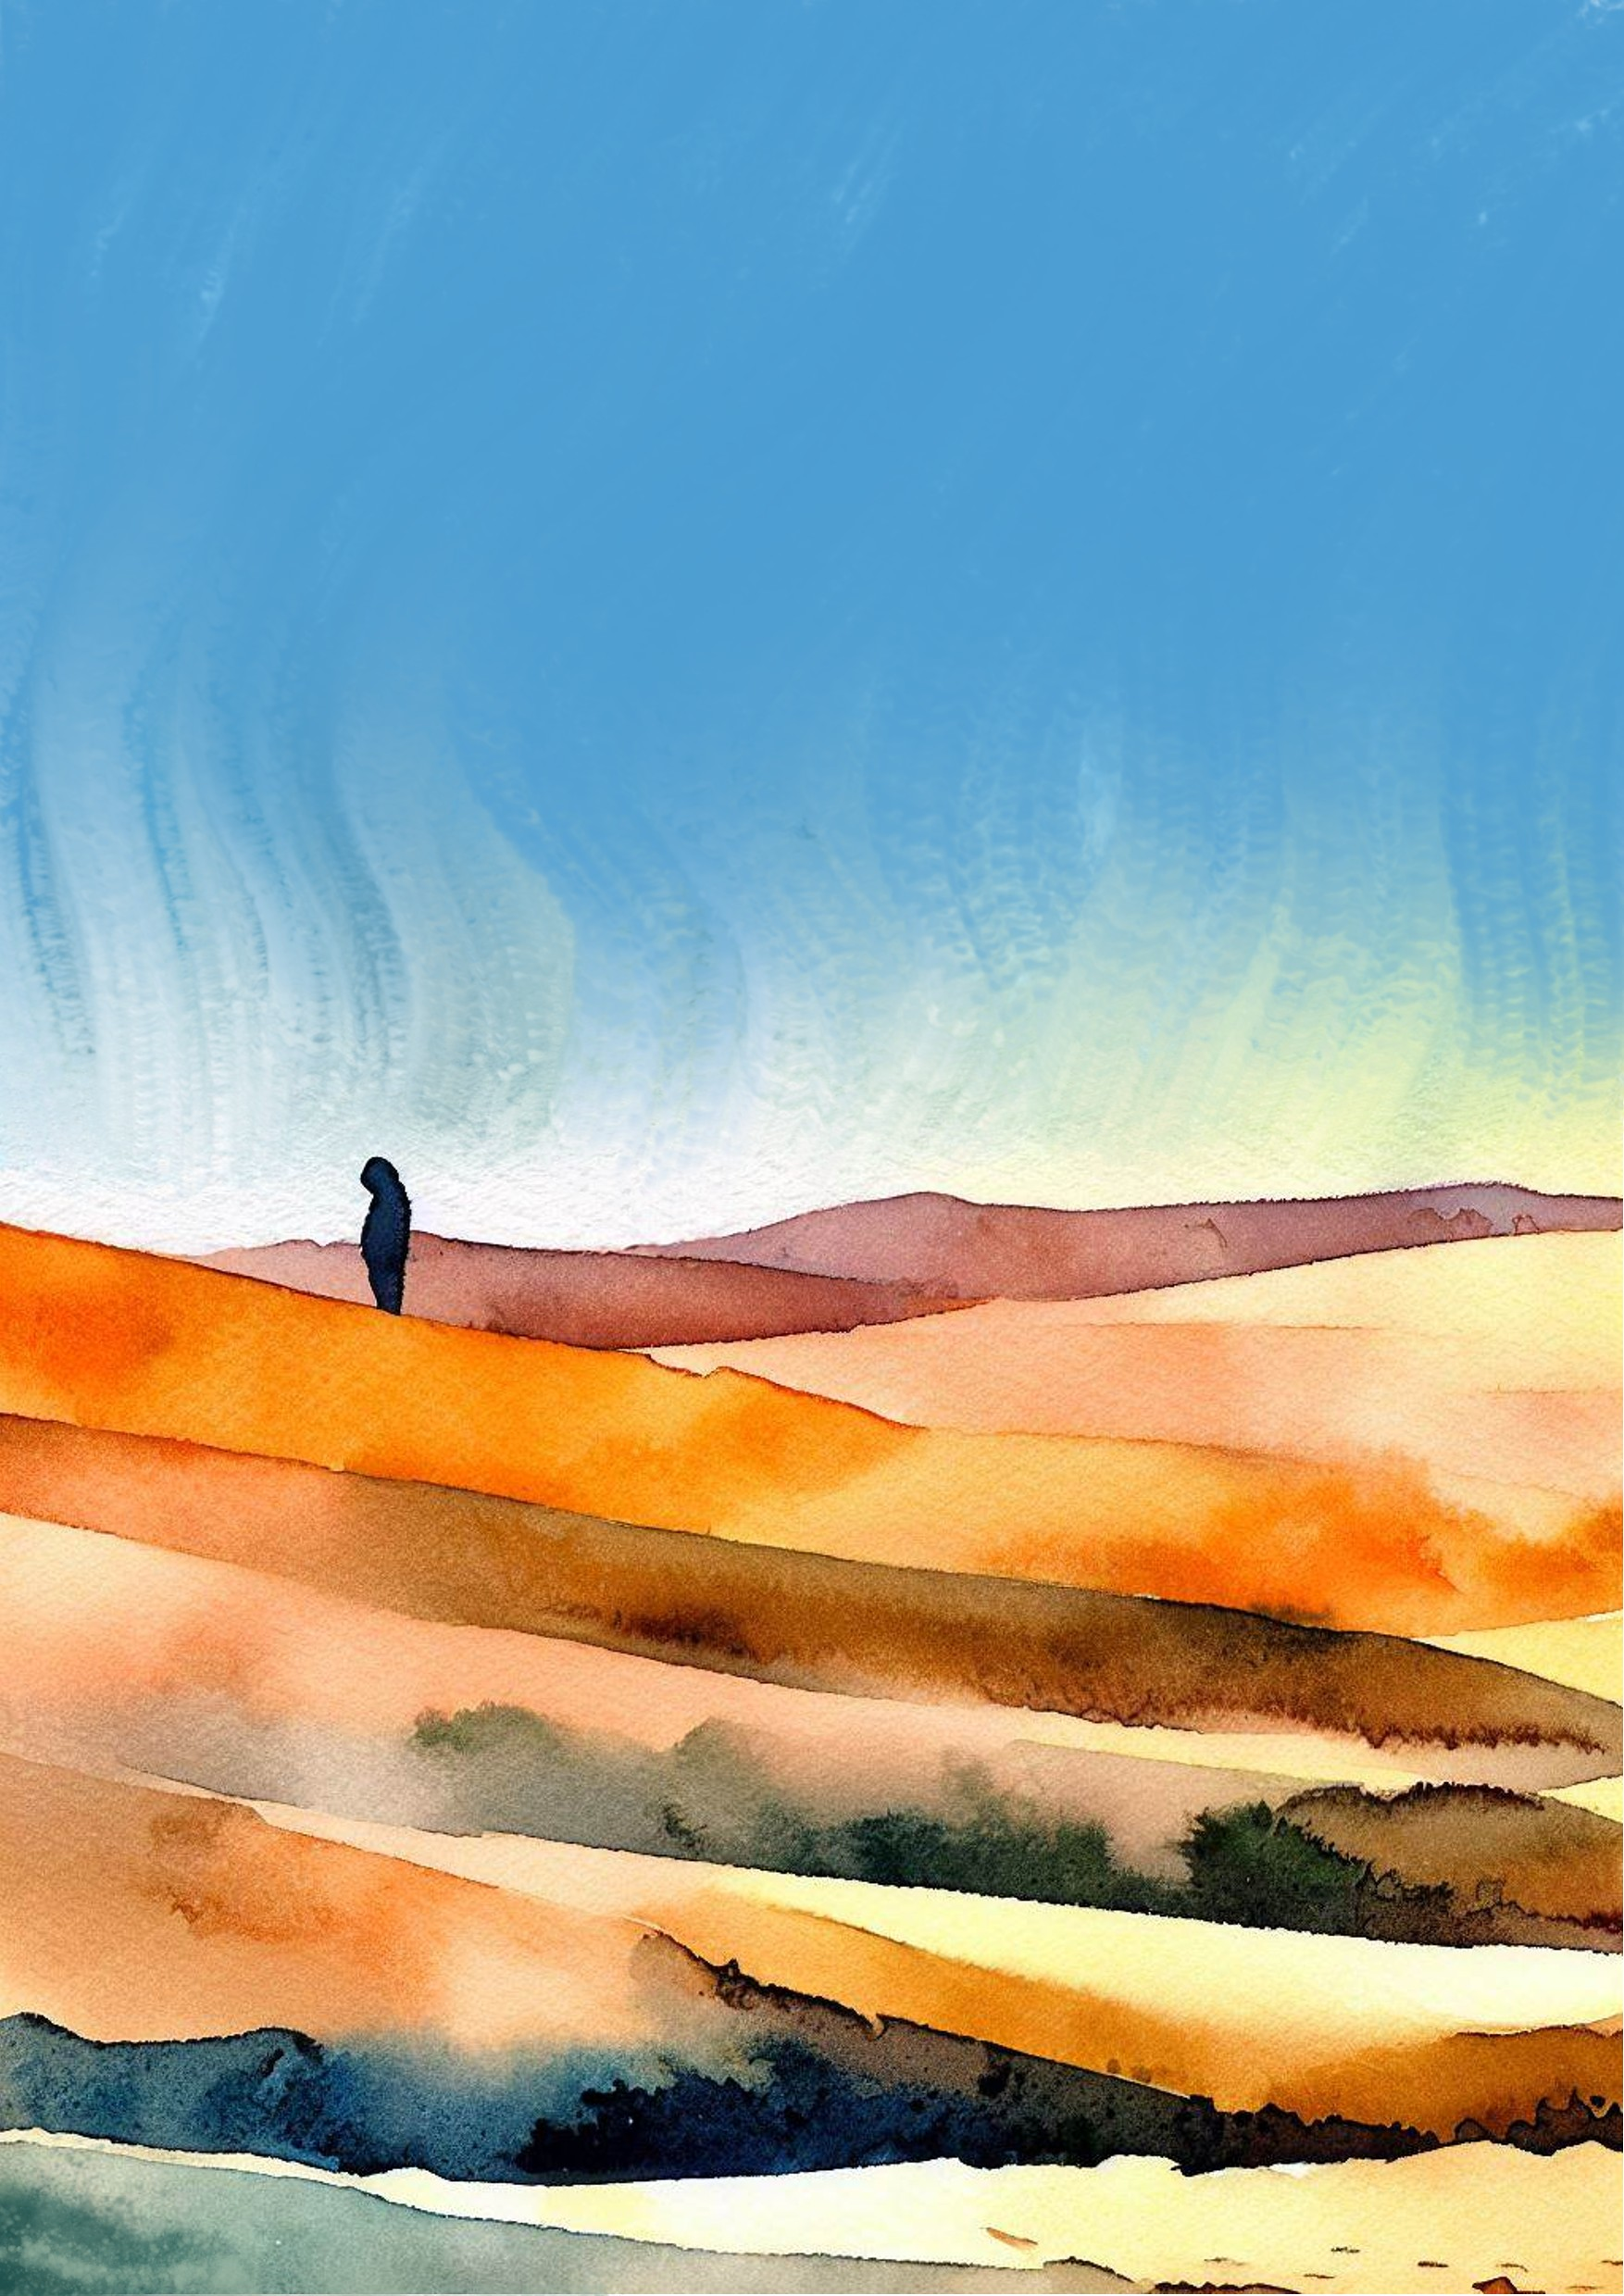
\includegraphics[width = \paperwidth, height = \paperheight] {images/endless-dunes}}}
\BgThispage
\newpage


\color{white}
\PlainPoemTitle
\PoemTitle{Сафари по Сахаре}

\begin{verse}[\versewidth]
Говорят что в Африке опасно. \\
Говорят ходить туда нельзя. \\
Говорят, конечно-же, напрасно, \\
Я там был, и всё совсем не так!
\end{verse}

\begin{verse}[\versewidth]
Расскажу я как дела в Сах\'{а}ре. \\
Объясню --- пустыня не пуста. \\
Покажу как там на самом деле. \\
Опишу, что кроется в песках.
\end{verse}


% \fancybreak{***}

\backgroundsetup{scale = 1, angle = 0, opacity = 1, contents = {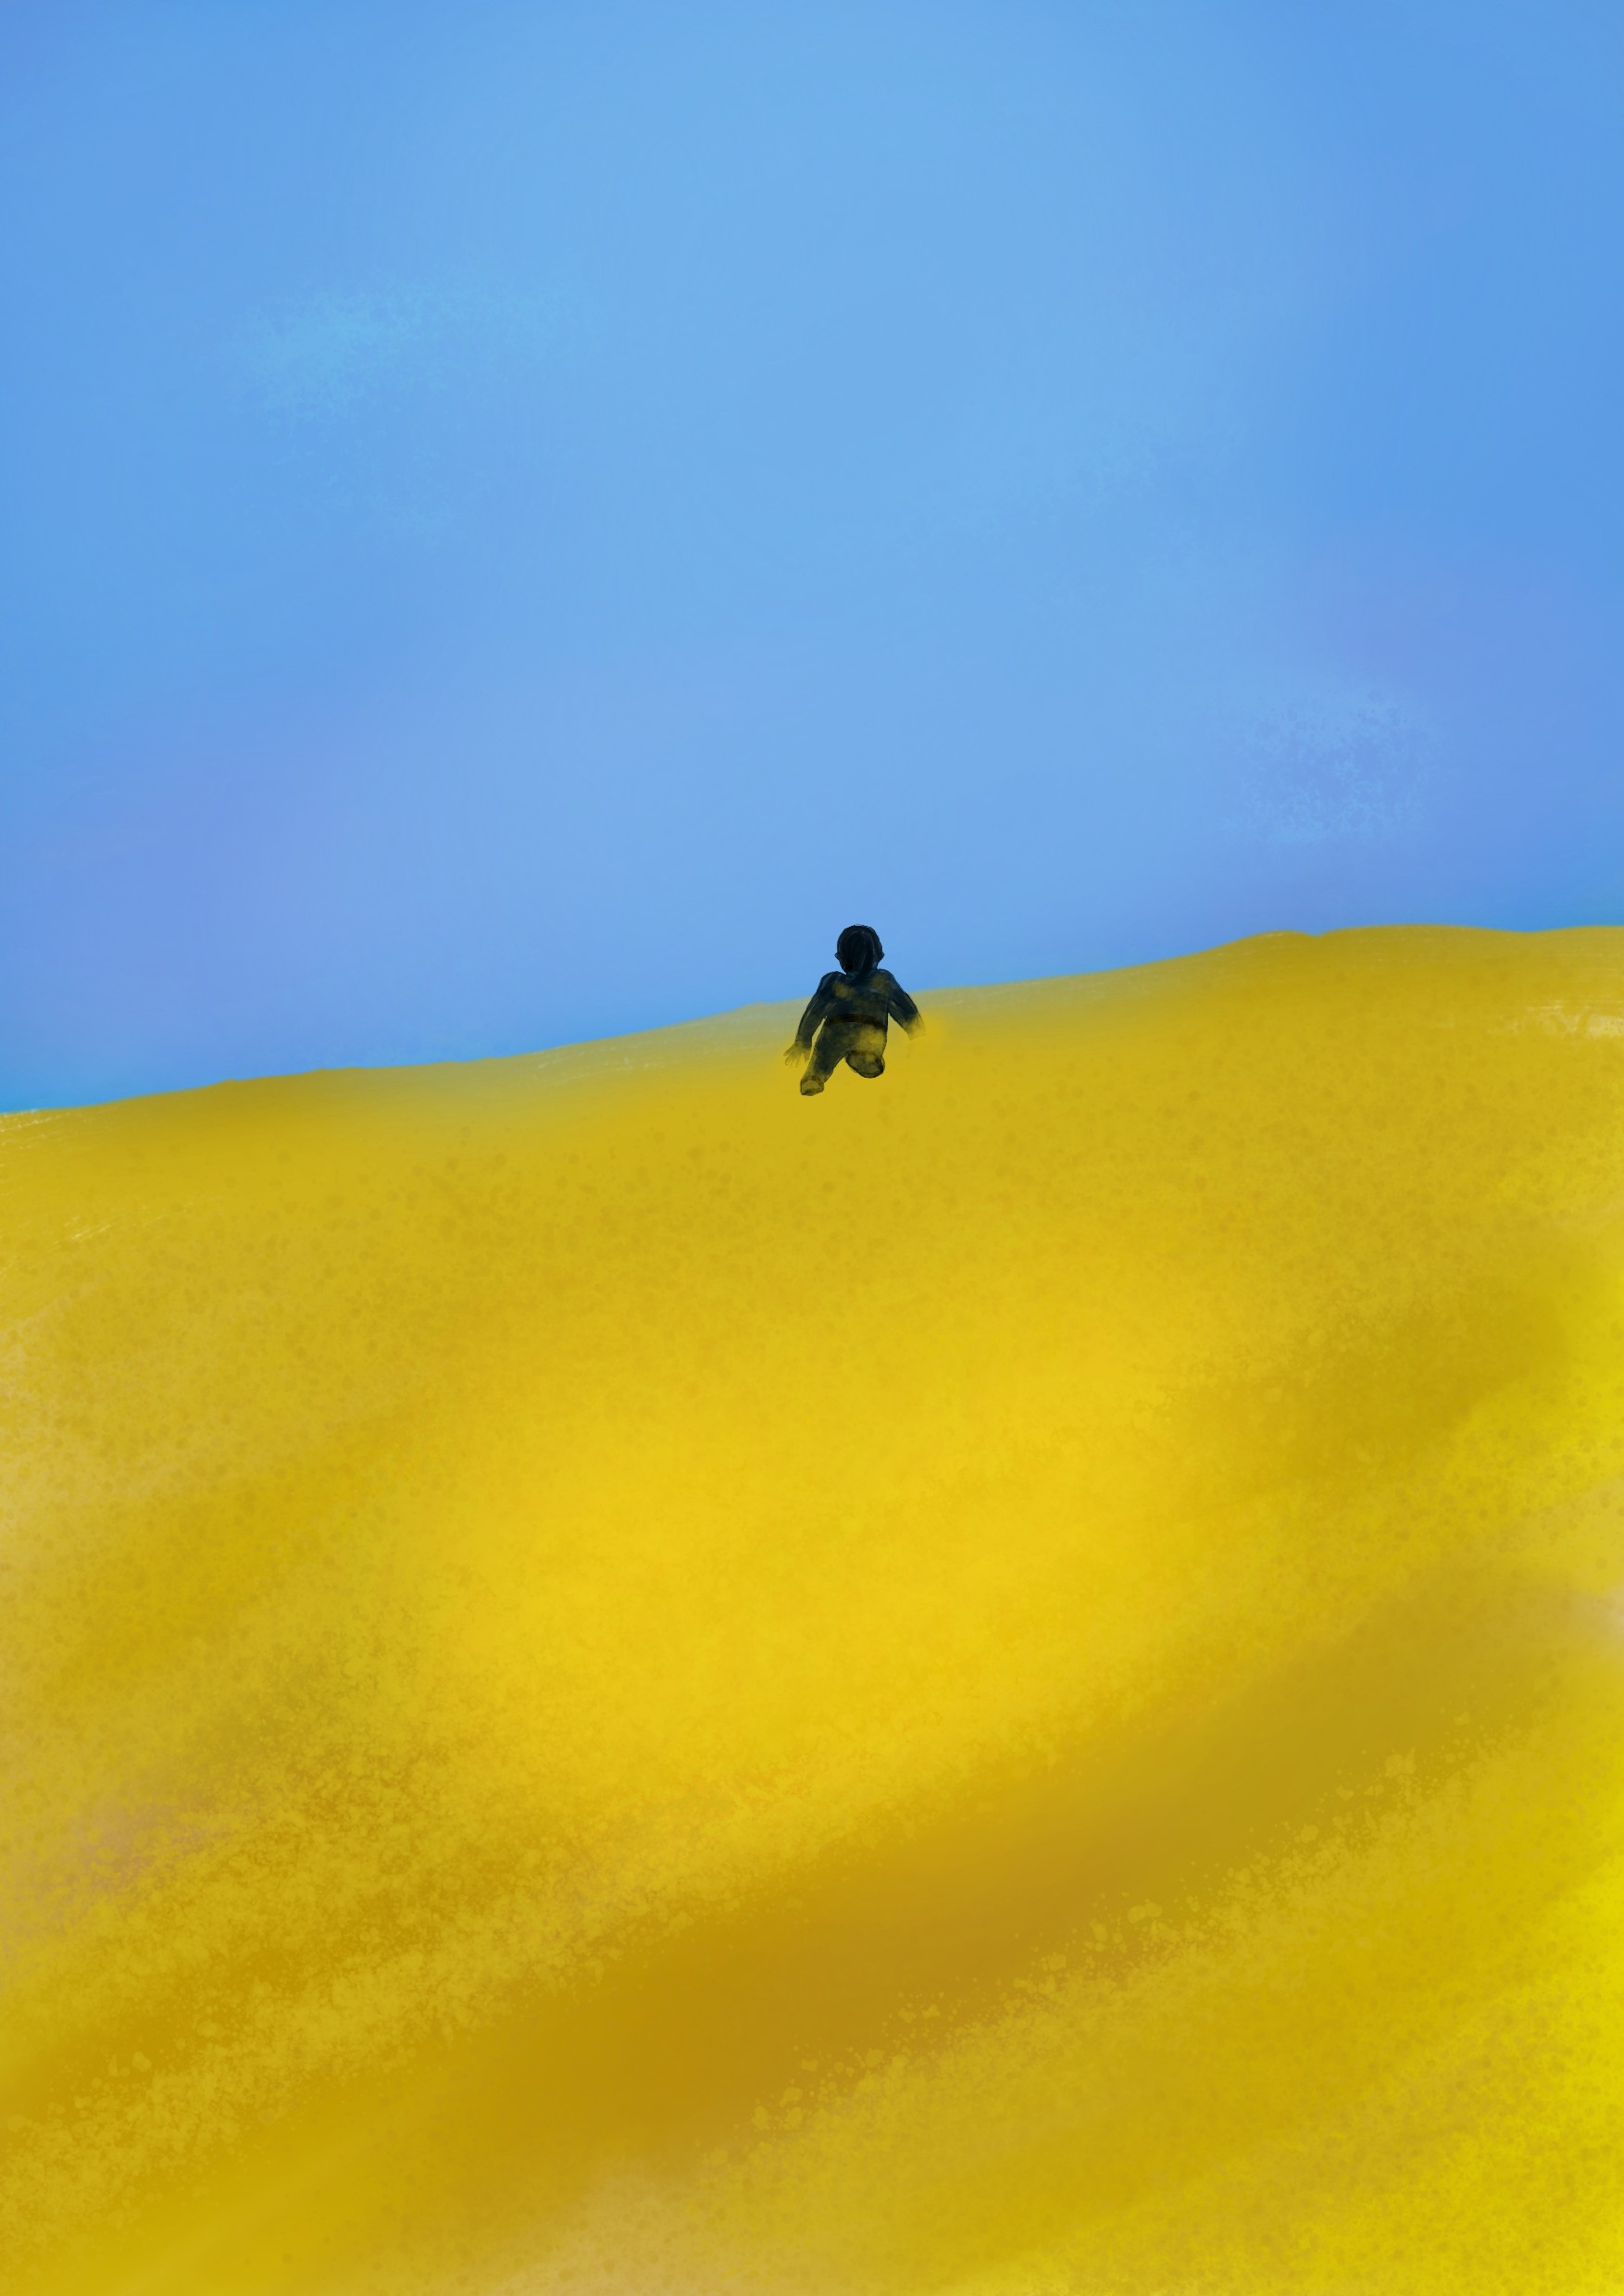
\includegraphics[width = \paperwidth, height = \paperheight] {images/interworld-dot}}}
\BgThispage

\vspace{4cm}
\color{black}
\begin{verse}[\versewidth]
От Атлантики, где солнце исчезает, \\
на восток, до моря из солей, \\
крупнейшая песочница планеты \\
ждёт в гостях людей и их детей.
\end{verse}

\begin{verse}[\versewidth]
Дюны, без конца, до горизонта \\
словно волны в океане из песка. \\
Терпеливо, ветер гонит по-крупинке, \\
через год --- ландшафта не узнать\ldots
\end{verse}

\begin{verse}[\versewidth]
Облаков почти не видно в синем небе, \\
а вода, что ты заметил --- лишь мираж. \\
Бесконечность сверху, бесконечность снизу, \\
ну а ты всего лишь точка в двух мирах.
\end{verse}

\newpage


\color{white}
\begin{verse}[\versewidth]
Гляди! Сюда идут другие точки! \\
Их силуэты с каждым шагом всё видней! \\
Возьми бинокль, посмотри получше, \\
узнаёшь горбатых ты зверей?
\end{verse}

\begin{verse}[\versewidth]
Конечно! Это же верблюды! \\
Они по дюнам ходят не спеша. \\
Им не нужны ни карты, ни приборы, \\
% пустыня им без знаков хороша.
для них пустыня вся --- дорожный знак.
\end{verse}

\begin{verse}[\versewidth]
А где верблюды --- там и туар\'{е}ги, \\
в инд\'{и}говых накидках и платках. \\
Они торгуют золотом и солью, \\
и сочиняют песни о песках.
\end{verse}

\backgroundsetup{scale = 1, angle = 0, opacity = 1, contents = {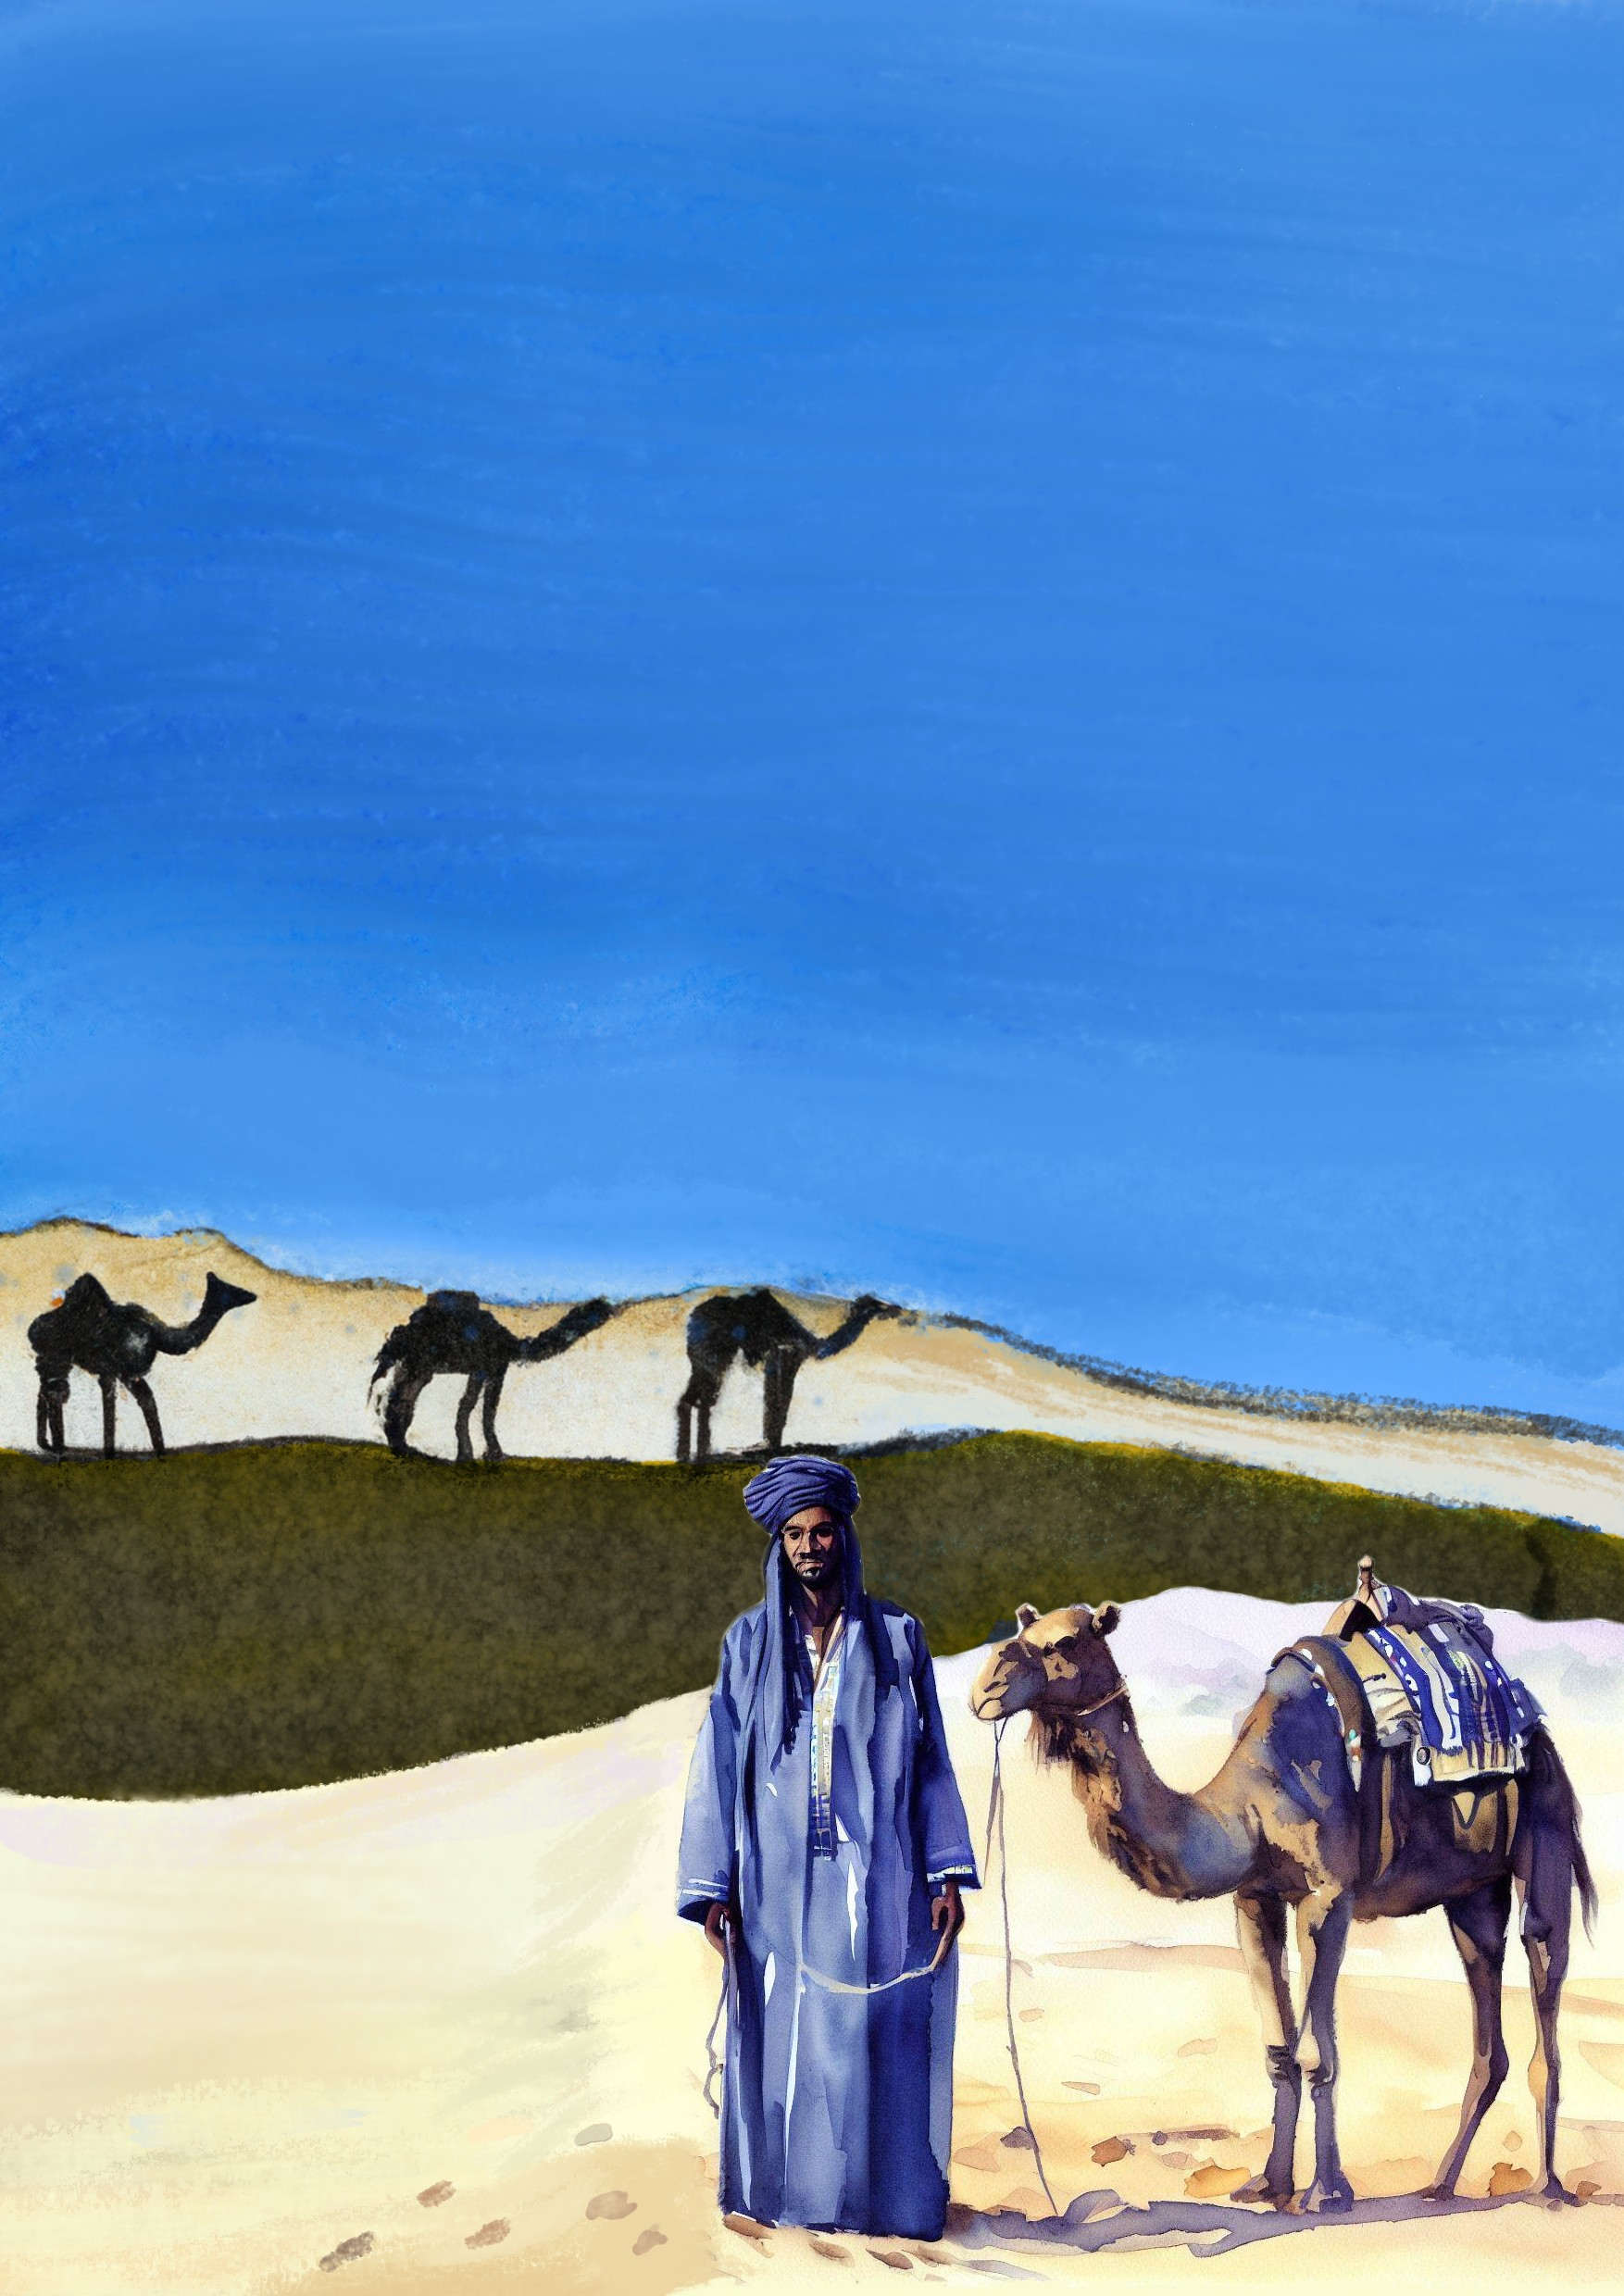
\includegraphics[width = \paperwidth, height = \paperheight] {images/caravan-daylight-touareg}}}
\BgThispage

\newpage
\color{black}
\begin{verse}[\versewidth]
Смотри под ноги, узнаёшь следы? \\
Недавно кто-то тут ходил. \\
Шакал? Ушастый ф\'{е}нек? Или ящер? \\
Может тушканчик тут бродил?
\end{verse}

\begin{verse}[\versewidth]
Прислушайся, что-то скрипит! \\
Как будто ходит вслед за нами, \\
невидимый, но верный друг, \\
точь-в-точь шагая вместе с нами!
\end{verse}

\begin{verse}[\versewidth]
Скрипит как снег, но где сугробы? \\
Ведь солнце жарит как в печи! \\
В Сах\'{а}ре лето круглый год, \\
так что-же всё-таки звучит?
\end{verse}

\begin{verse}[\versewidth]
А скрип всё громче, и местами --- \\
он вырастает в громкий гул! \\
Не самолёт ли это в небе? \\
Рой саранч\'{и} к нам повернул?
\end{verse}

\begin{verse}[\versewidth]
Да да! Бывает и такое, \\
но не сейчас, ведь пусто всё вокруг! \\
Запомни, если нет дождя и сухо --- \\
то иногда пески поют!
\end{verse}
\fancybreak{***}

\backgroundsetup{scale = 1, angle = 0, opacity = 0.45, contents = {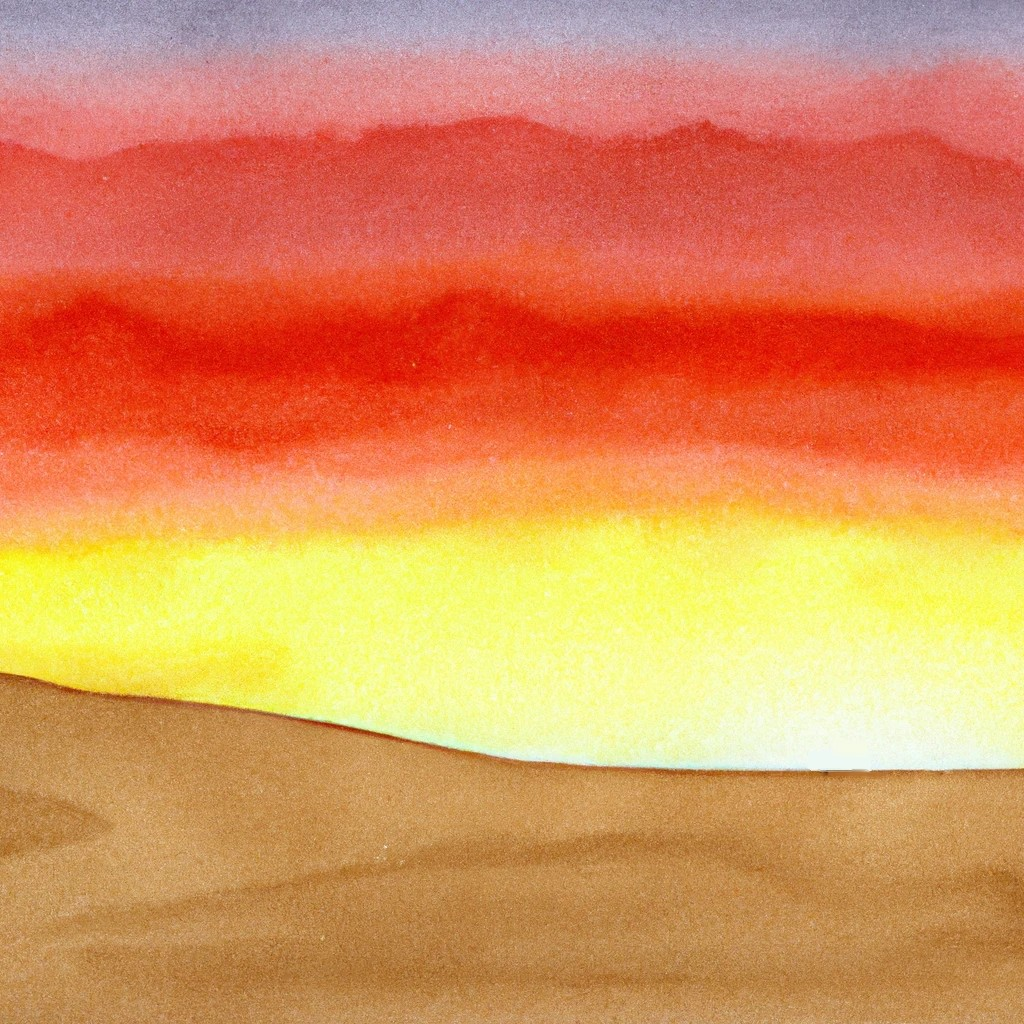
\includegraphics[width = \paperwidth, height = \paperheight] {images/sunset}}}
\BgThispage

\begin{verse}[\versewidth]
Летят минуты и часы, и небо пожелтело, \\
оранжев\'{е}я и краснея как пожар. \\
Вокруг всё плавно затемнело, \\
и ночь остановила солнца жар.
\end{verse}

\begin{verse}[\versewidth]
На небосводе загорелись звёзды, \\
% и полумесяц ярко заблестел
и бледно завиднелася луна. \\
Галактики, туманности, планеты, \\
гуляют по орбитам сквозь века.
\end{verse}


\begin{verse}[\versewidth]
К костру поближе-ка присядь, \\
ведь холод наступает. \\
Горячего чайку попей, \\
он быстро согревает!
\end{verse}

\begin{verse}[\versewidth]
А перед тем как глаз замкнуть \\
проверь палатку дважды --- \\
чтоб змеям внутрь путь закрыть, \\
да скорпионам всяким\ldots
\end{verse}

\begin{verse}[\versewidth]
Всмотрись в Полярную звезду \\
и посчитай до ста, \\
когда дойдешь до тридцати \\
наступит время сна.
\end{verse}
% \hfill

\backgroundsetup{scale = 1, angle = 0, opacity = 0.45, contents = {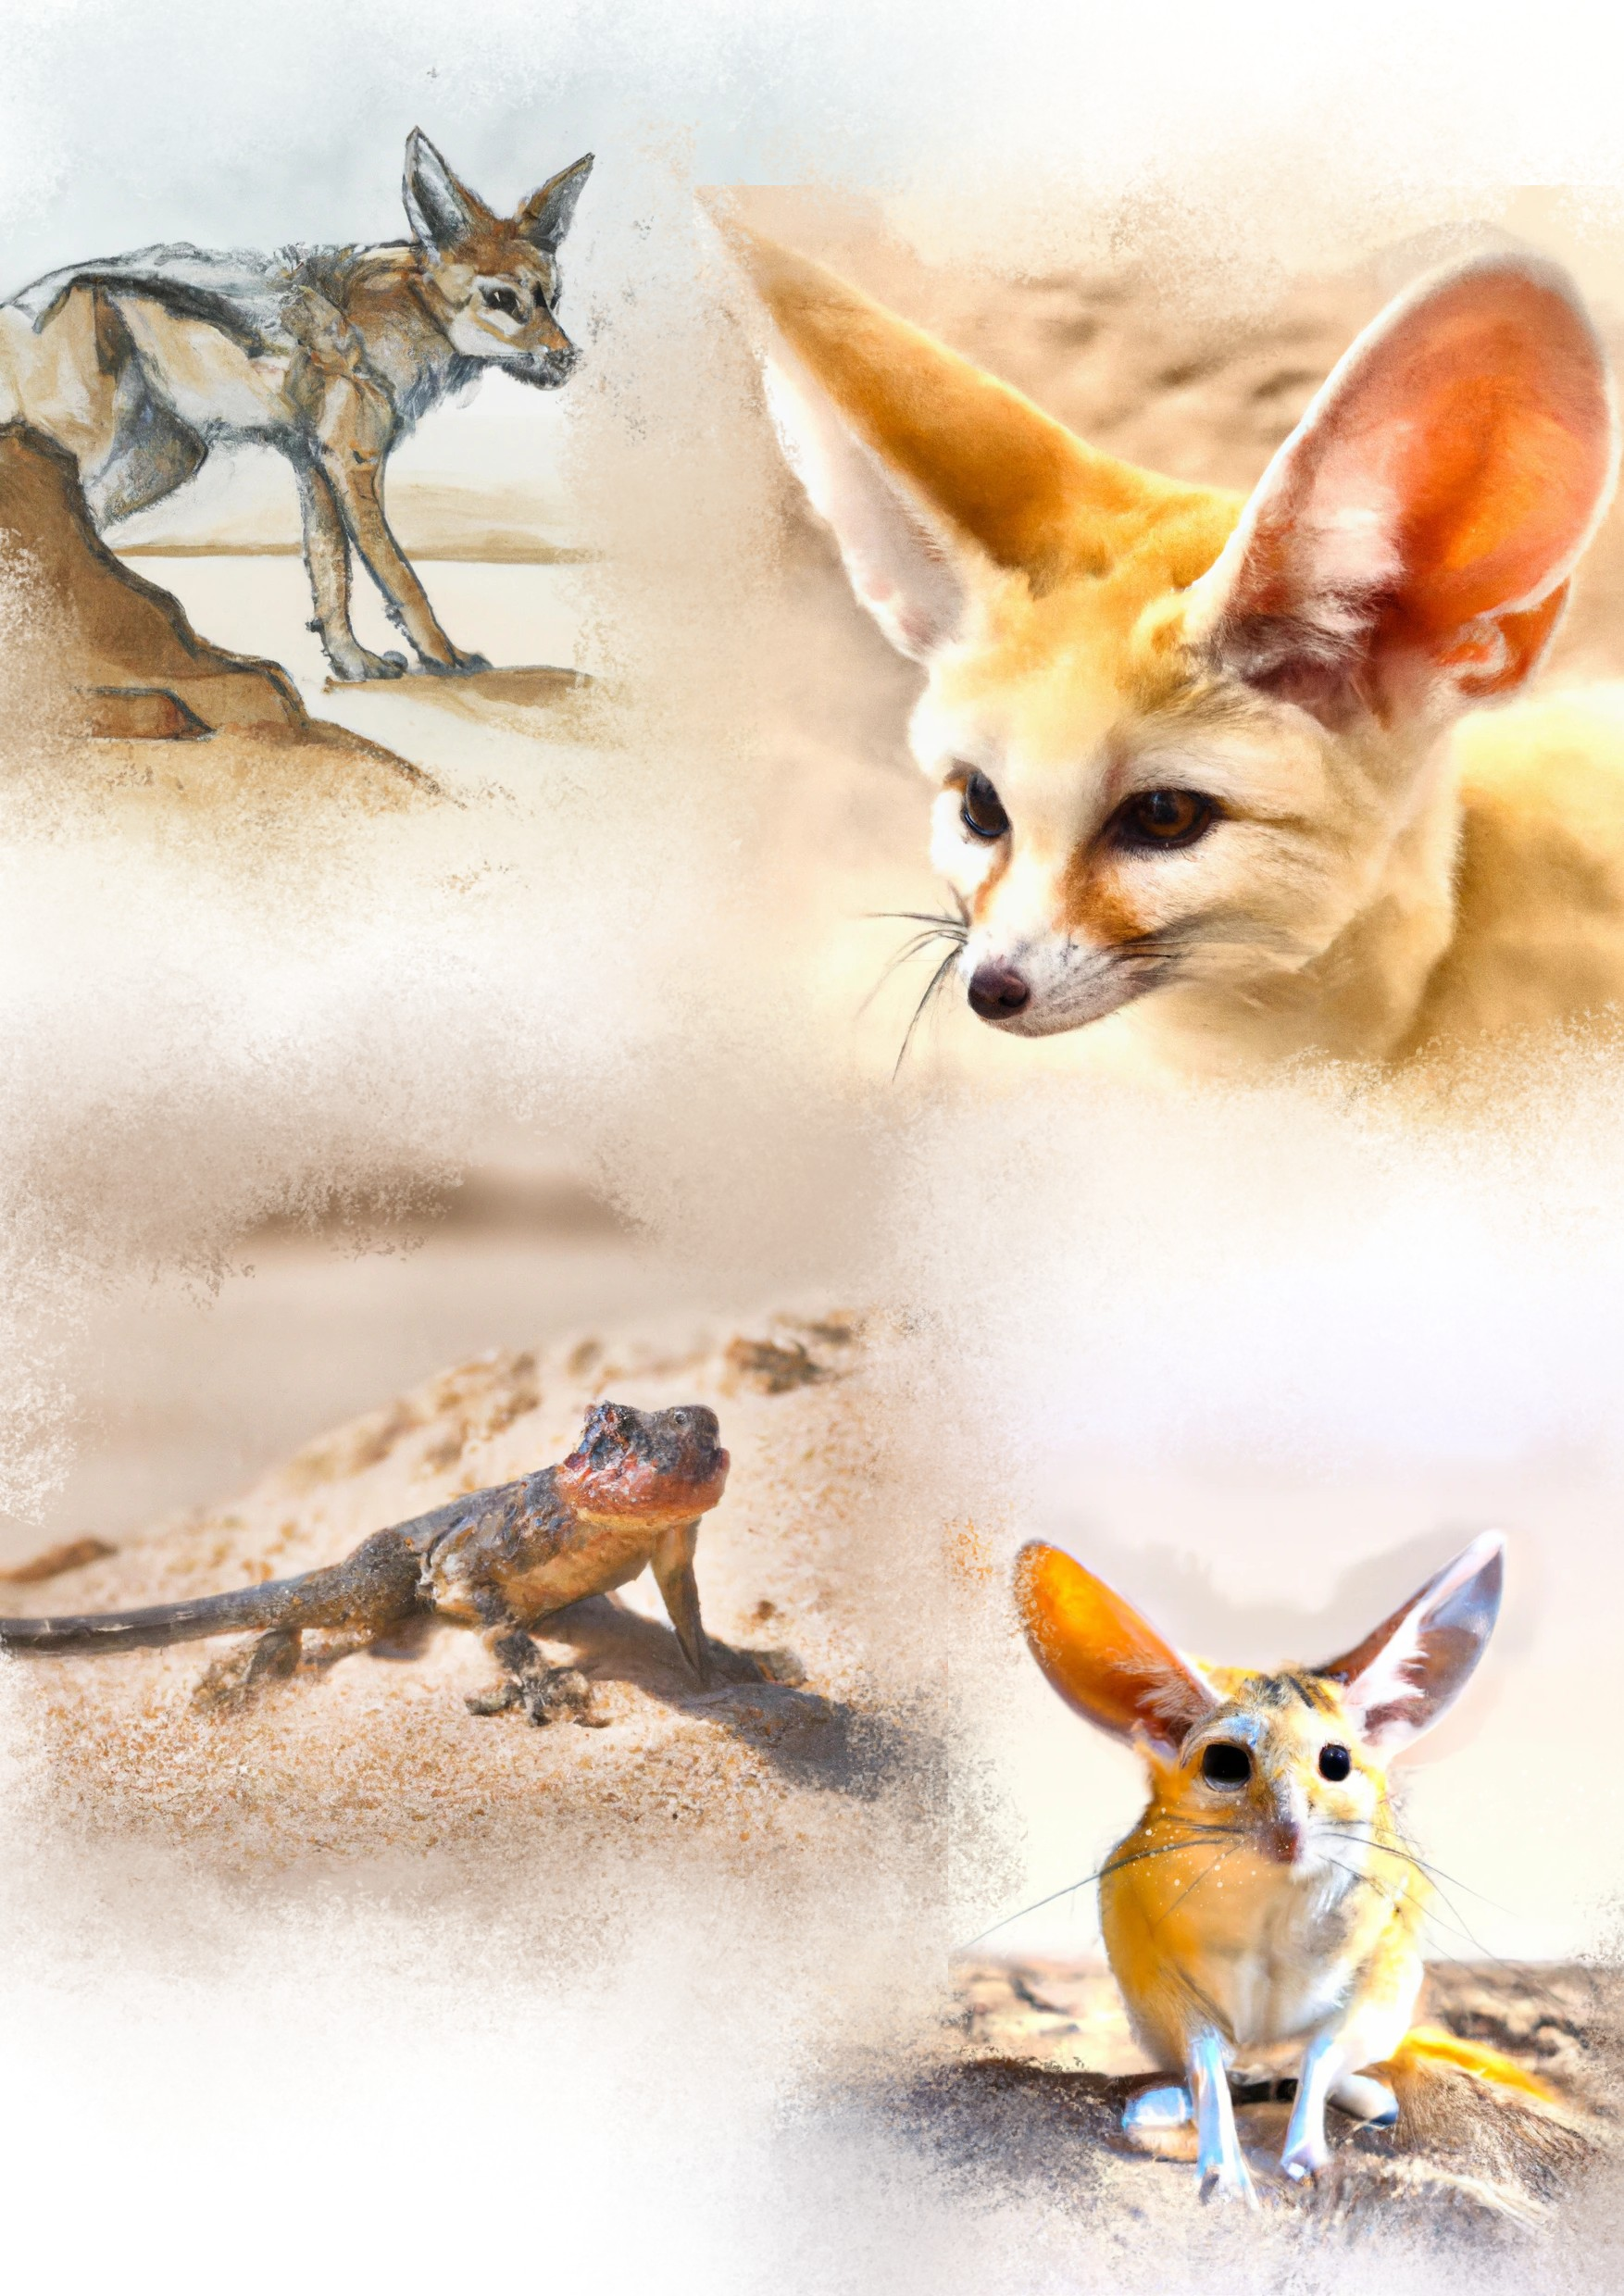
\includegraphics[width = \paperwidth, height = \paperheight] {images/sahara-animal-collage}}}
\BgThispage

\newpage
% Location: In Amenas, 24 Feb 2023 @20:00
% Facing ~North	
% https://stellarium-web.org/skysource/Polaris?fov=138.05&date=2023-02-24T18:24:19Z&lat=28.04&lng=9.58&elev=0
\backgroundsetup{scale = 1, angle = 0, opacity = 1, contents = {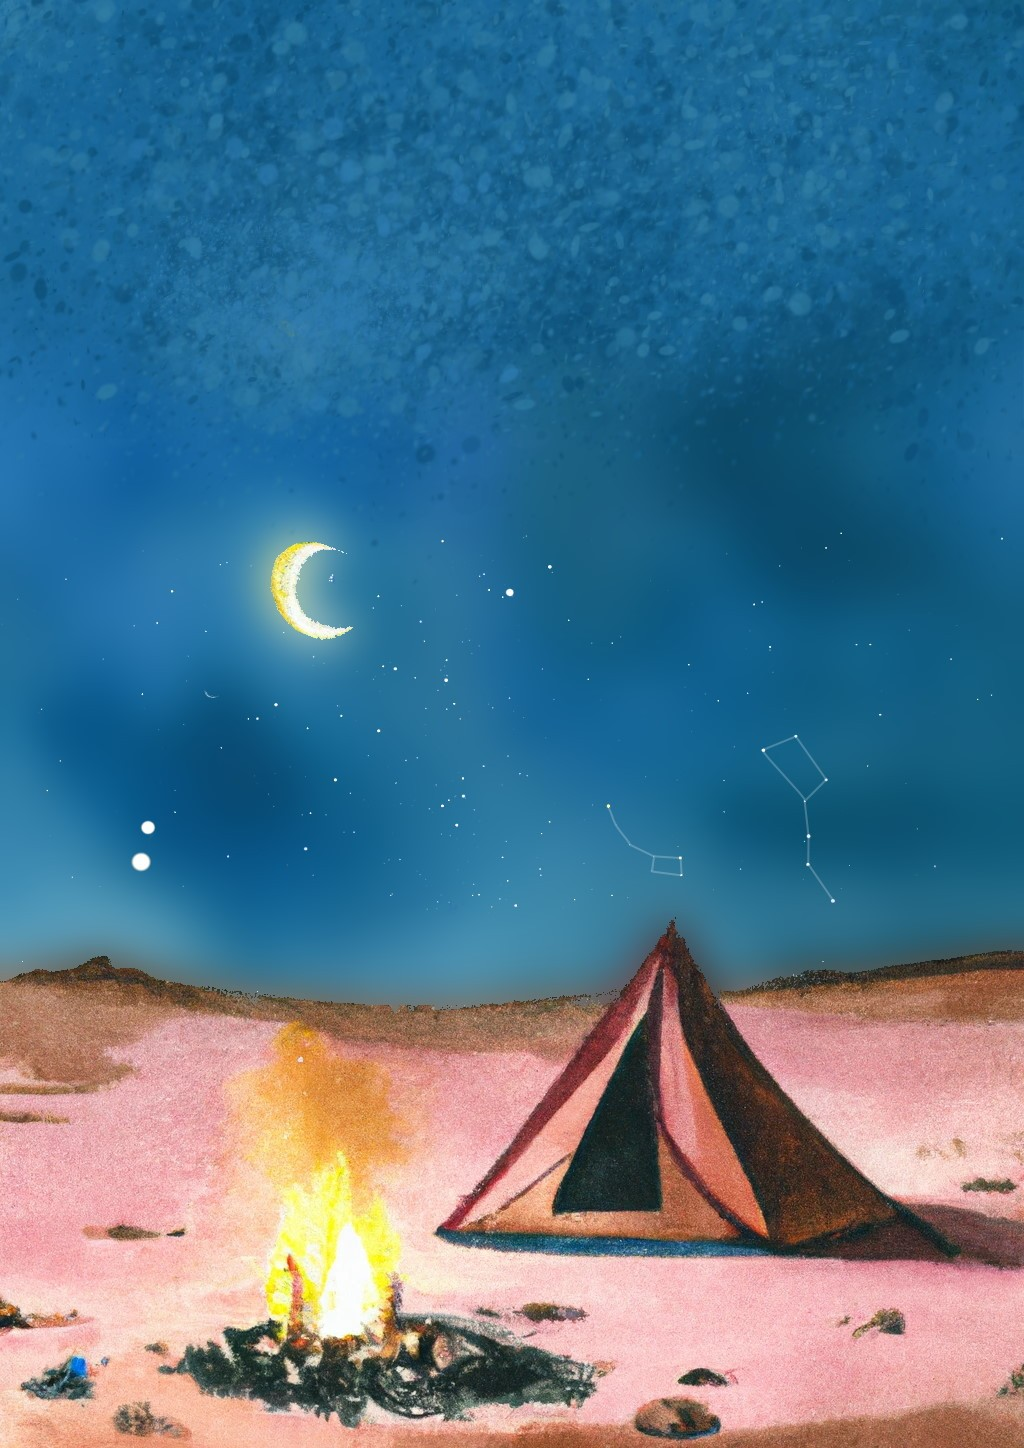
\includegraphics[width = \paperwidth, height = \paperheight] {images/night-sky-before-constellations}}}
\BgThispage
\color{white}
\begin{verse}[\versewidth]
Закружатся созвездия, \\
и в космо--хоровод, \\
затянут мигом и тебя --- \\
ведь космос всех зовёт!
\end{verse}

\begin{verse}[\versewidth]
Ты полетишь над облаками, \\
над пальмами и городами, \\
над в\'{а}ди, над горами, \\
%\hspace{-50mm}в одной только пижаме!
%в одной только пижаме!
в твоей сиреневой пижаме!
\end{verse}

\fancybreak{***}

\begin{verse}[\versewidth]
\hspace{1cm} Приземлись в местечке Айн--Аминас, \\
\hspace{1cm} под финиковой пальмой отдохни. \\
\hspace{1cm} Дай финик фенеку, да и сама попробуй, \\
\hspace{1cm} песчанку свежей фигой угости\ldots
\end{verse}


\begin{verse}[\versewidth]
\hspace{1cm} Пройдись по оазису, \\
\hspace{1cm} бурдюк водой наполни. \\
\hspace{1cm} \emph{Розу Сахары} подбери в песках. \\
% \hspace{1cm} И вспомни ту сверх--древнюю эпоху --- \\
% \hspace{1cm} когда саванна процветала в сих местах\ldots\\
% \hspace{1cm} Когда вода текла рекой по в\'{а}ди, \\
% \hspace{1cm} а гельта была дельтой той реки. \\
% \hspace{1cm} Когда дожди её за край переполняли, \\
% \hspace{1cm} и рыбы в ней плескали плавники\ldots
\end{verse}

% \fancybreak{***}
\clearpage
\vspace*{3cm}
\color{black}
\begin{verse}[\versewidth]
И вспомни ту сверх--древнюю эпоху --- \\
когда саванна процветала в сих местах\ldots\\
Когда вода текла рекой по в\'{а}ди, \\
а гельта была дельтой той реки. \\
Когда дожди её за край переполняли, \\
и рыбы в ней плескали плавники\ldots
\end{verse}
% savannah collage is here LEFT
\backgroundsetup{scale = 1, angle = 0, opacity = 1, contents = {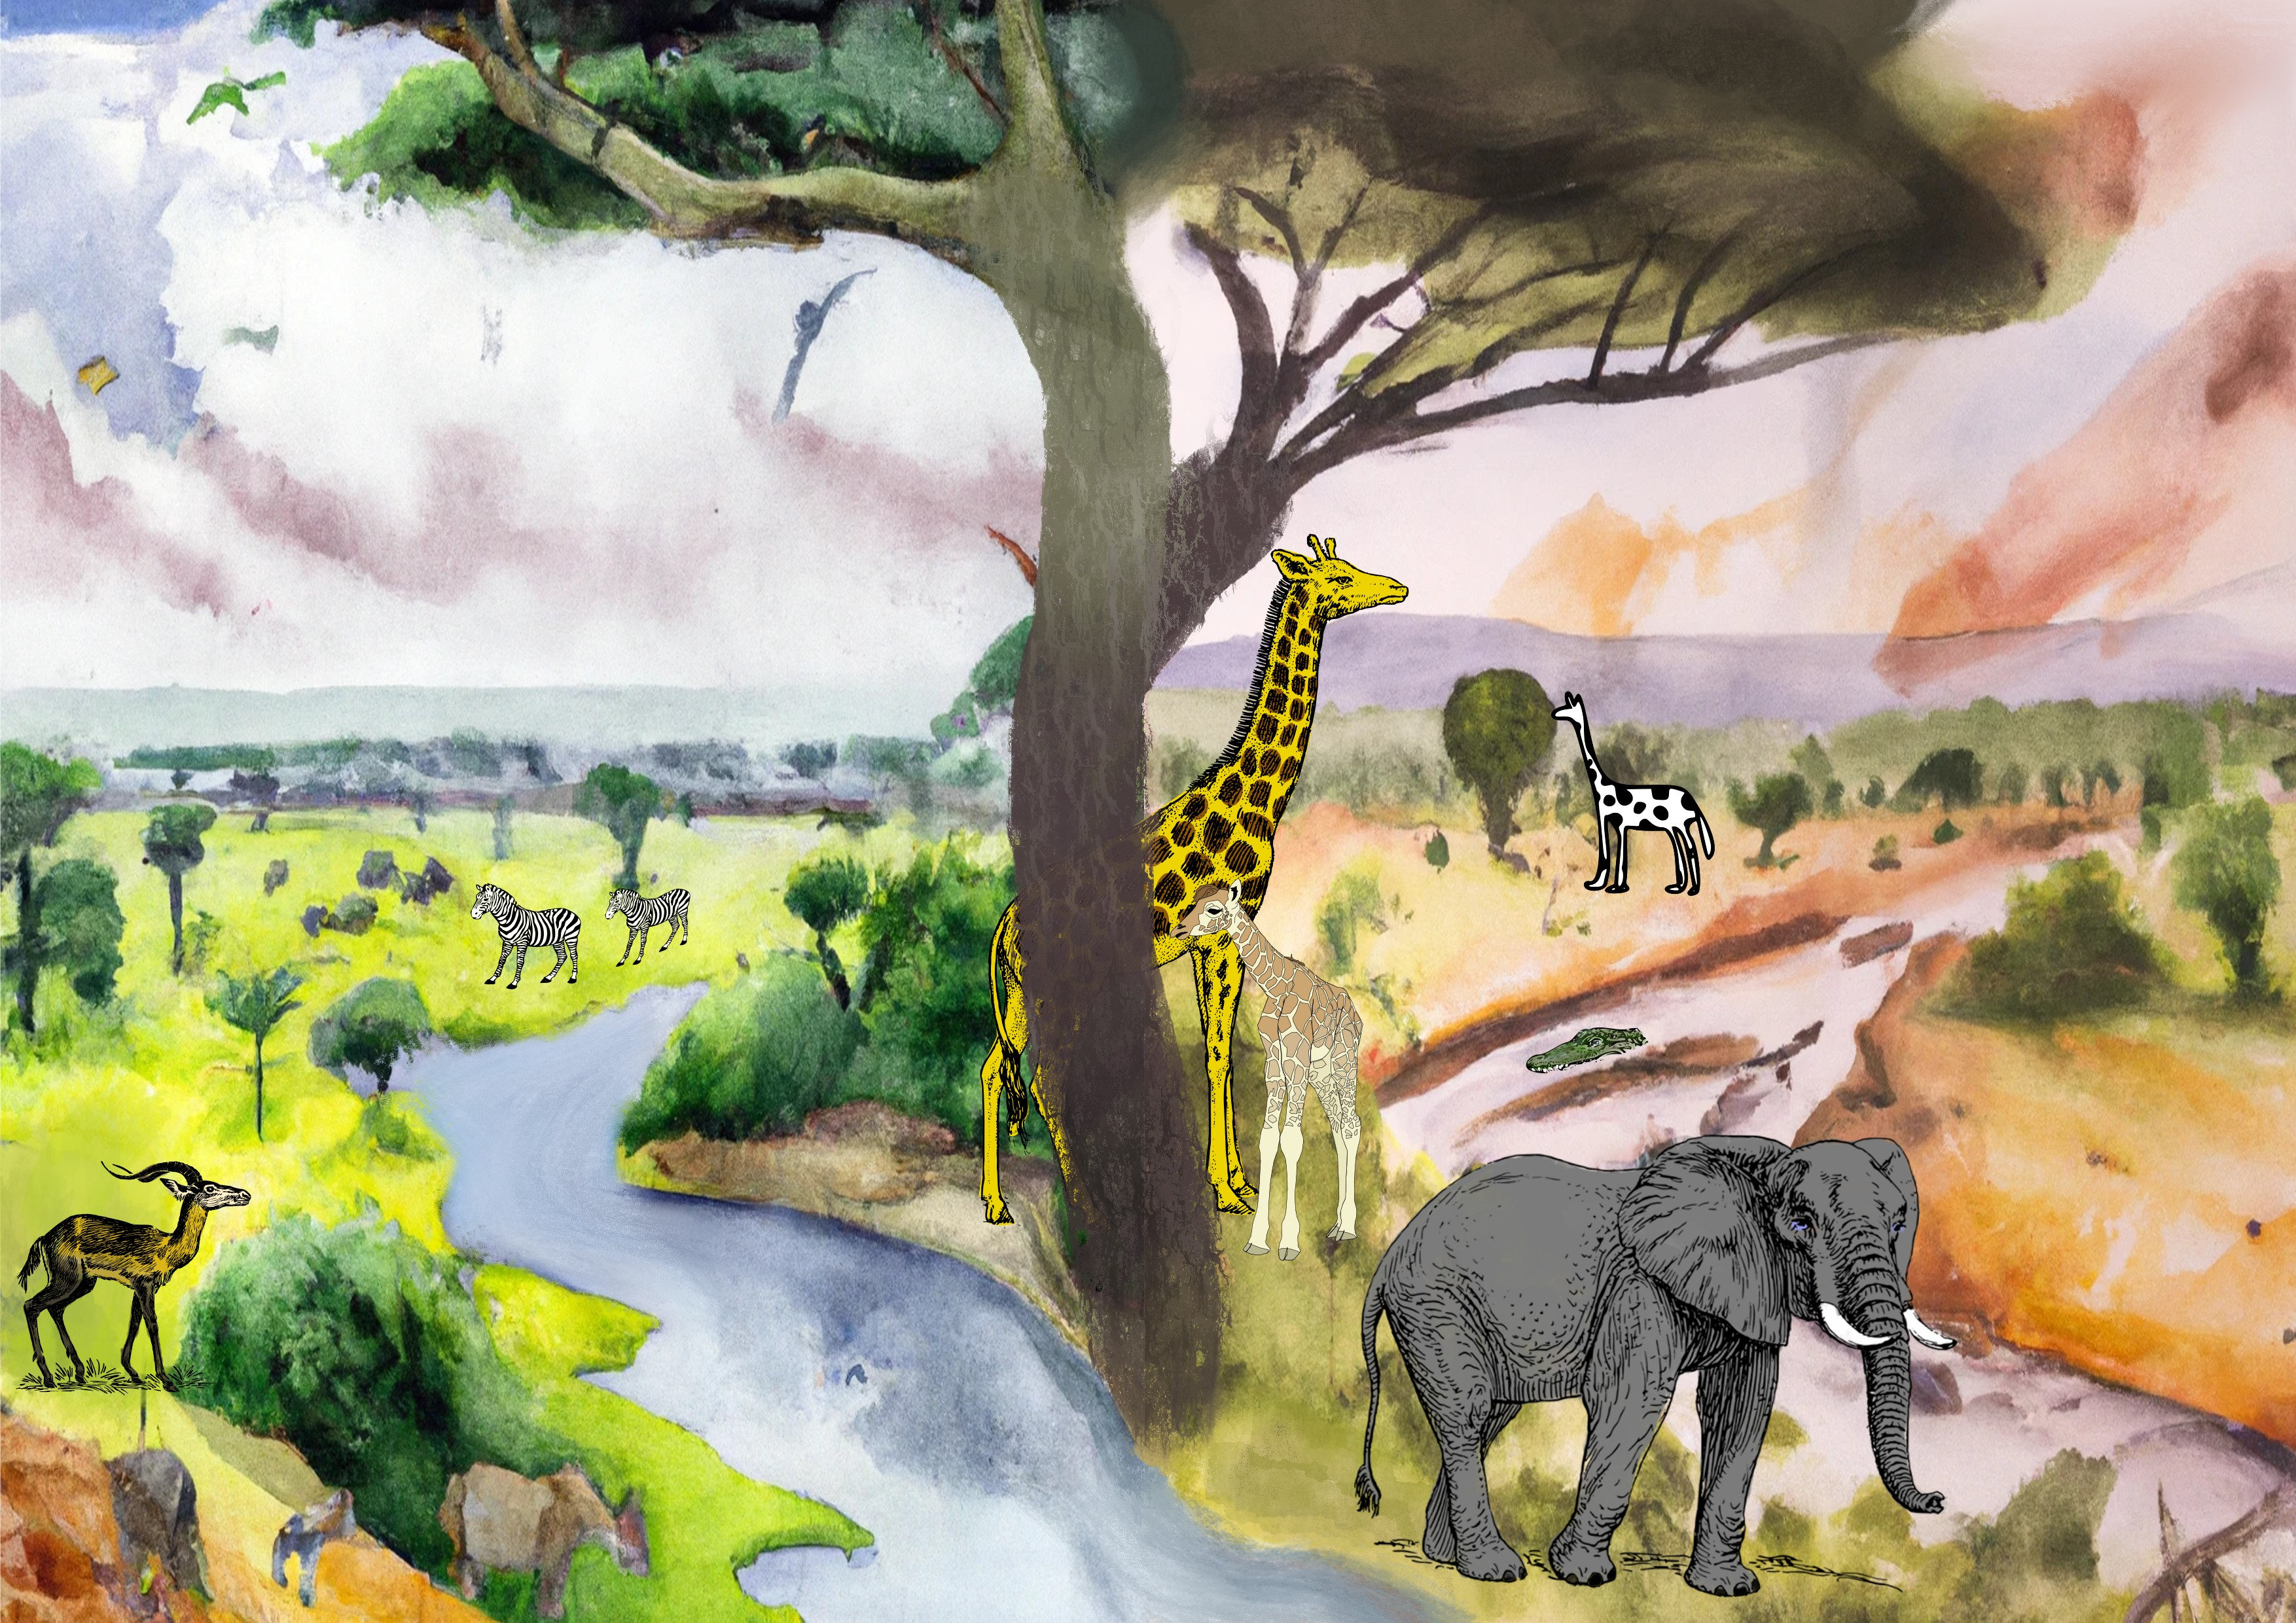
\includegraphics[width = \paperwidth, height = \paperheight,trim={0 0 148mm 0},clip] {images/savanna-collage}}}
\BgThispage

\newpage
\null
% savannah collage is here RIGHT
\backgroundsetup{scale = 1, angle = 0, opacity = 1, contents = {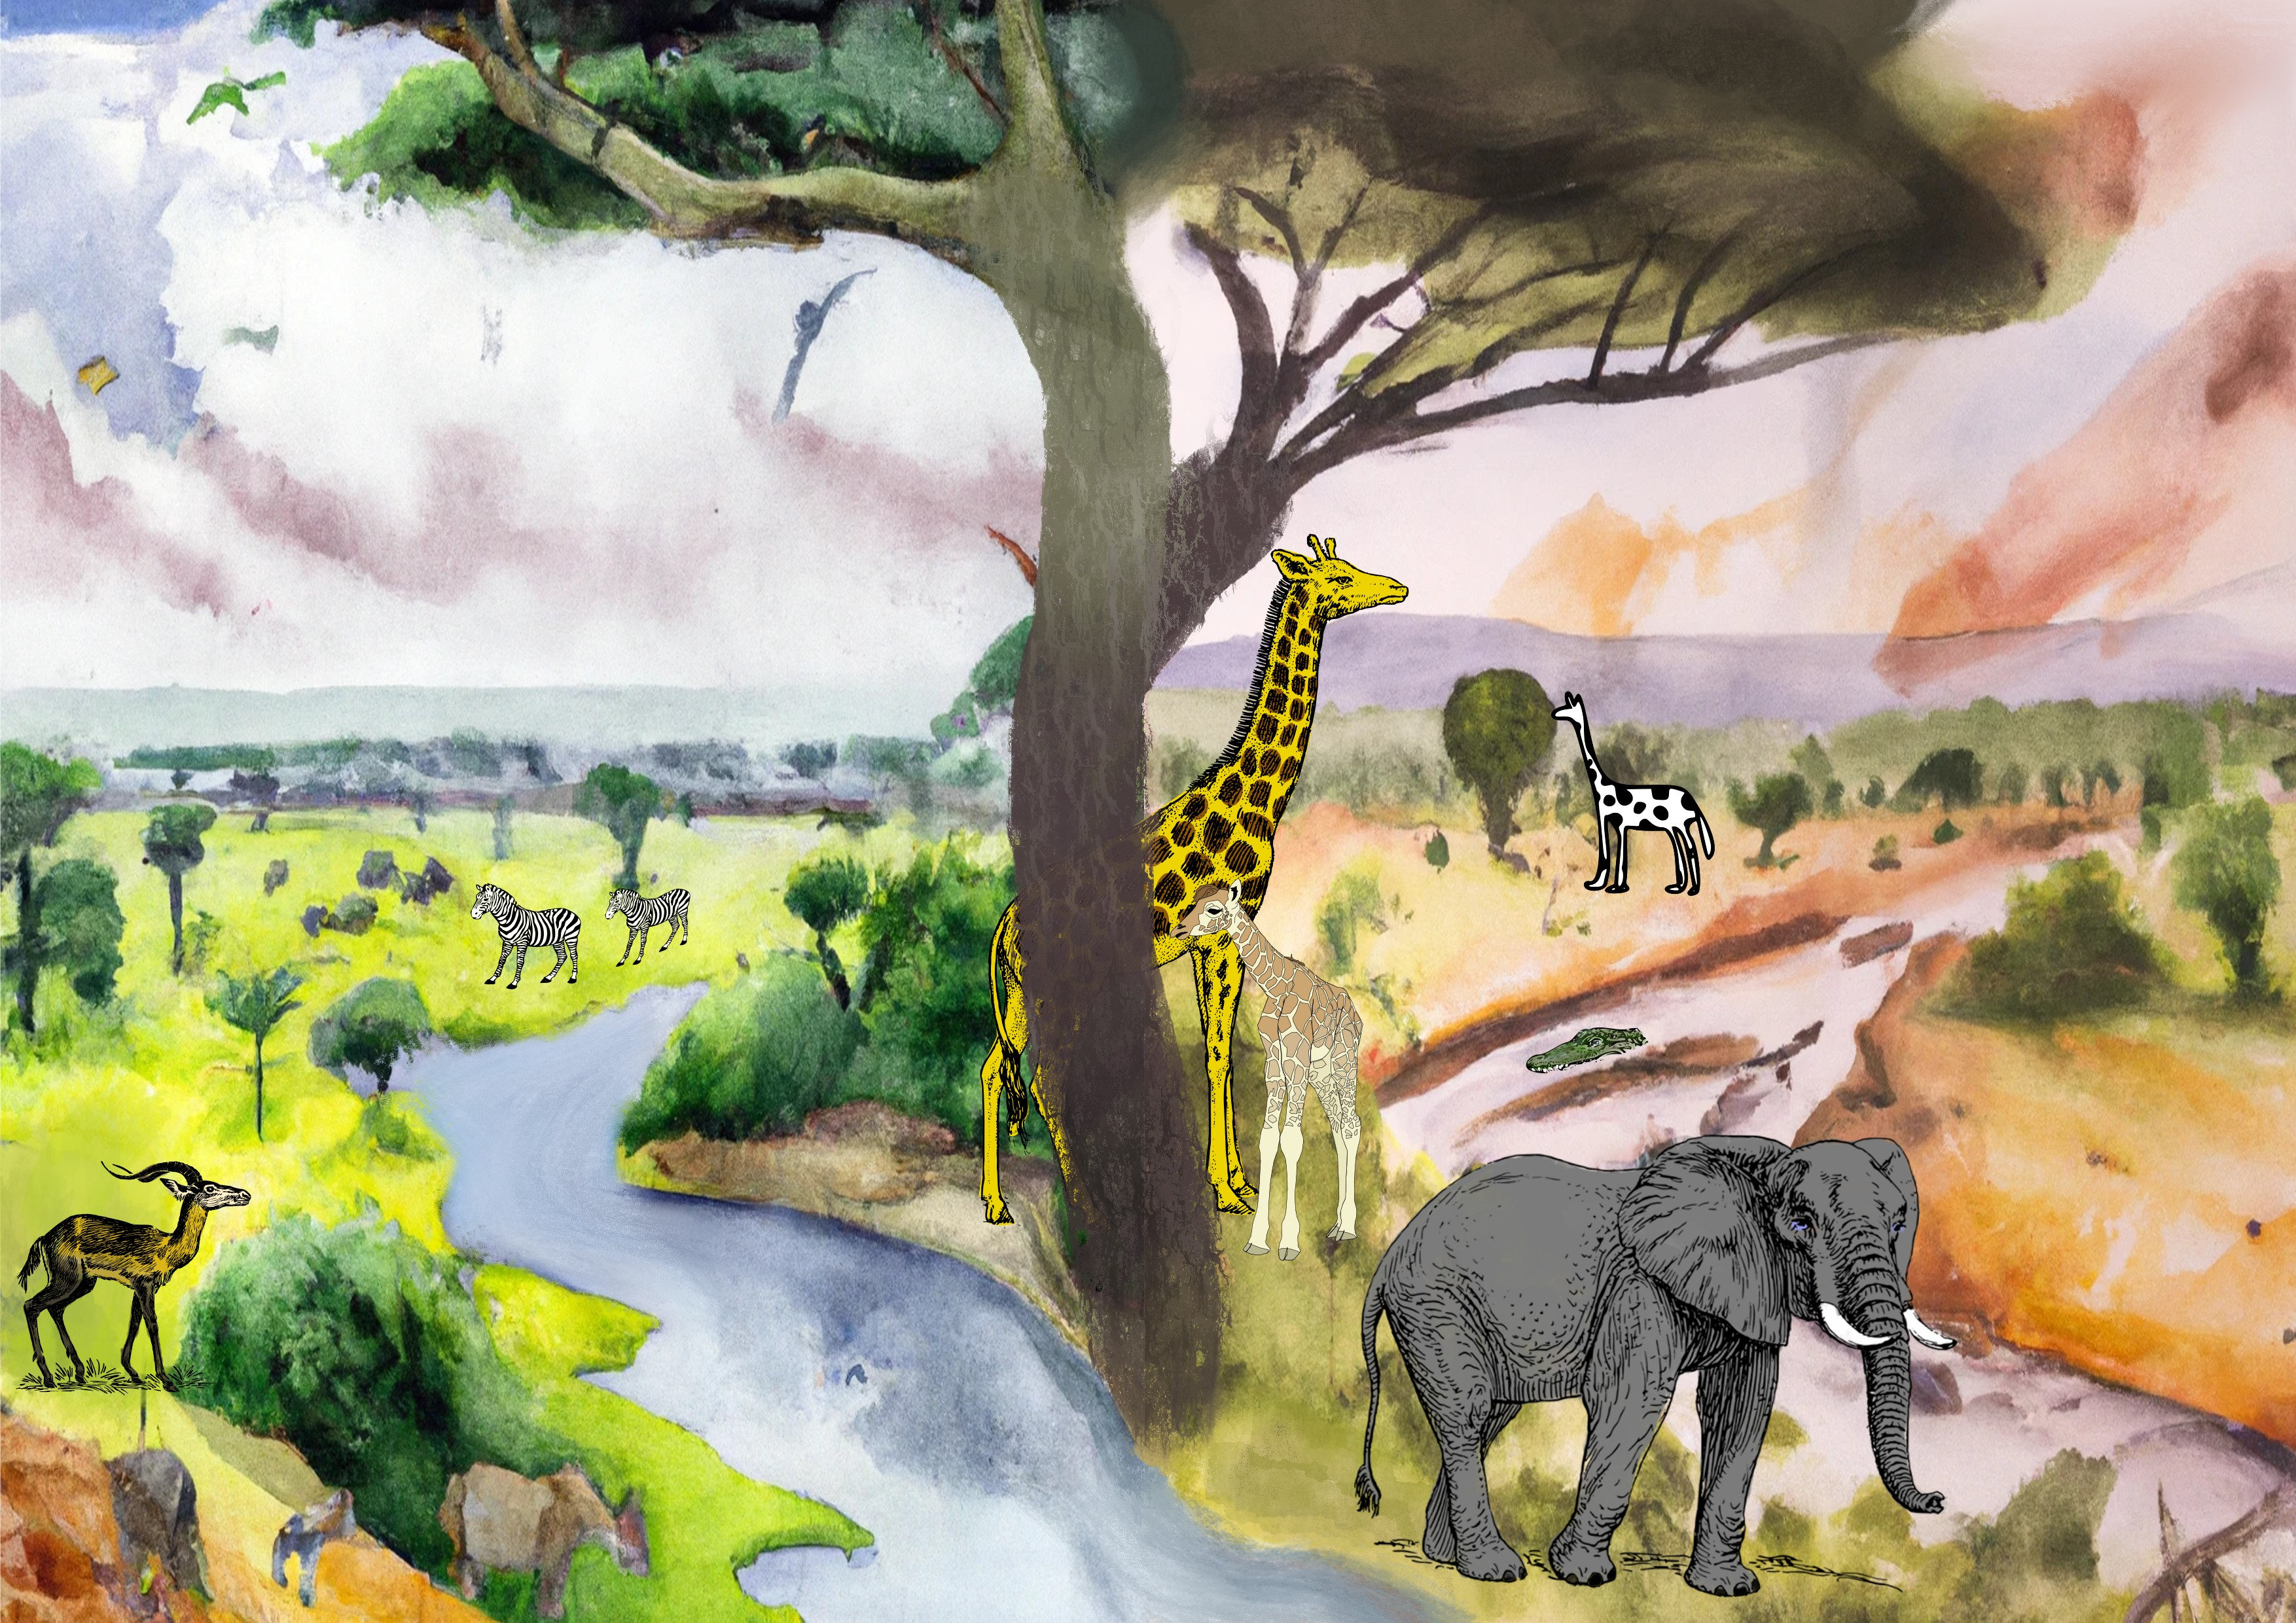
\includegraphics[width = \paperwidth, height = \paperheight,trim={148mm 0 0 0},clip] {images/savanna-collage}}}
\BgThispage

\newpage


\color{white}
\begin{verse}[\versewidth]
Время бежит, и утро наступает. \\
Проснувшись, ты опять среди песков. \\
И жажда о себе напоминает, \\
прервав бесцеремонно фазу снов.
\end{verse}
\color{black}
\backgroundsetup{scale = 1, angle = 0, opacity = 1, contents = {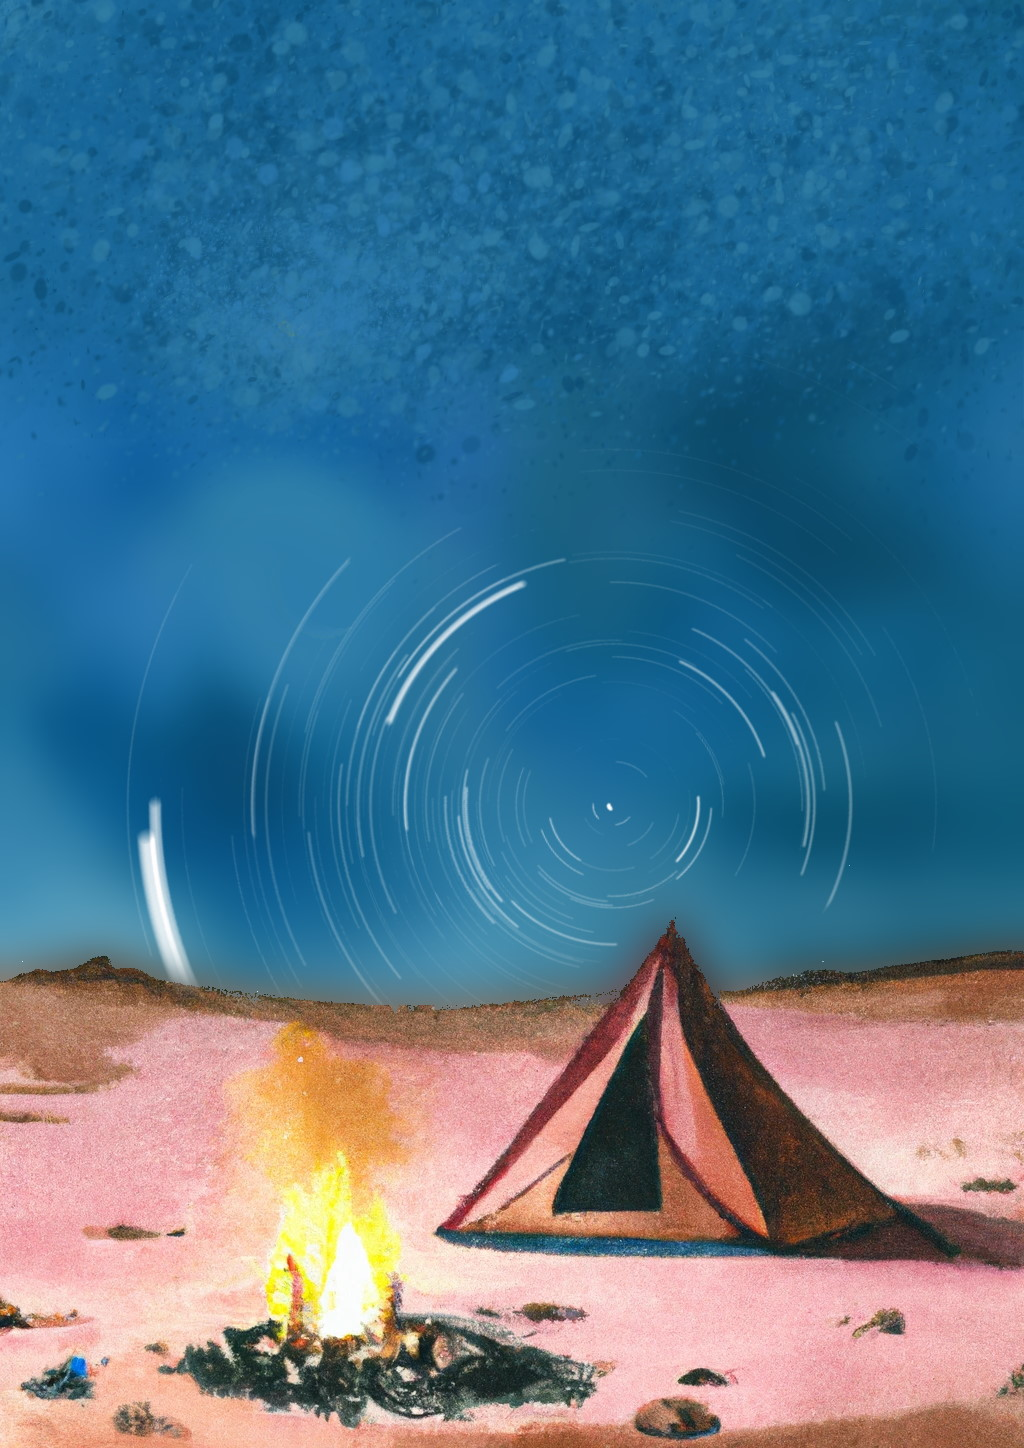
\includegraphics[width = \paperwidth, height = \paperheight] {images/night-sky-after}}}
\BgThispage

\newpage
\hfill
\backgroundsetup{scale = 1, angle = 0, opacity = 1, contents = {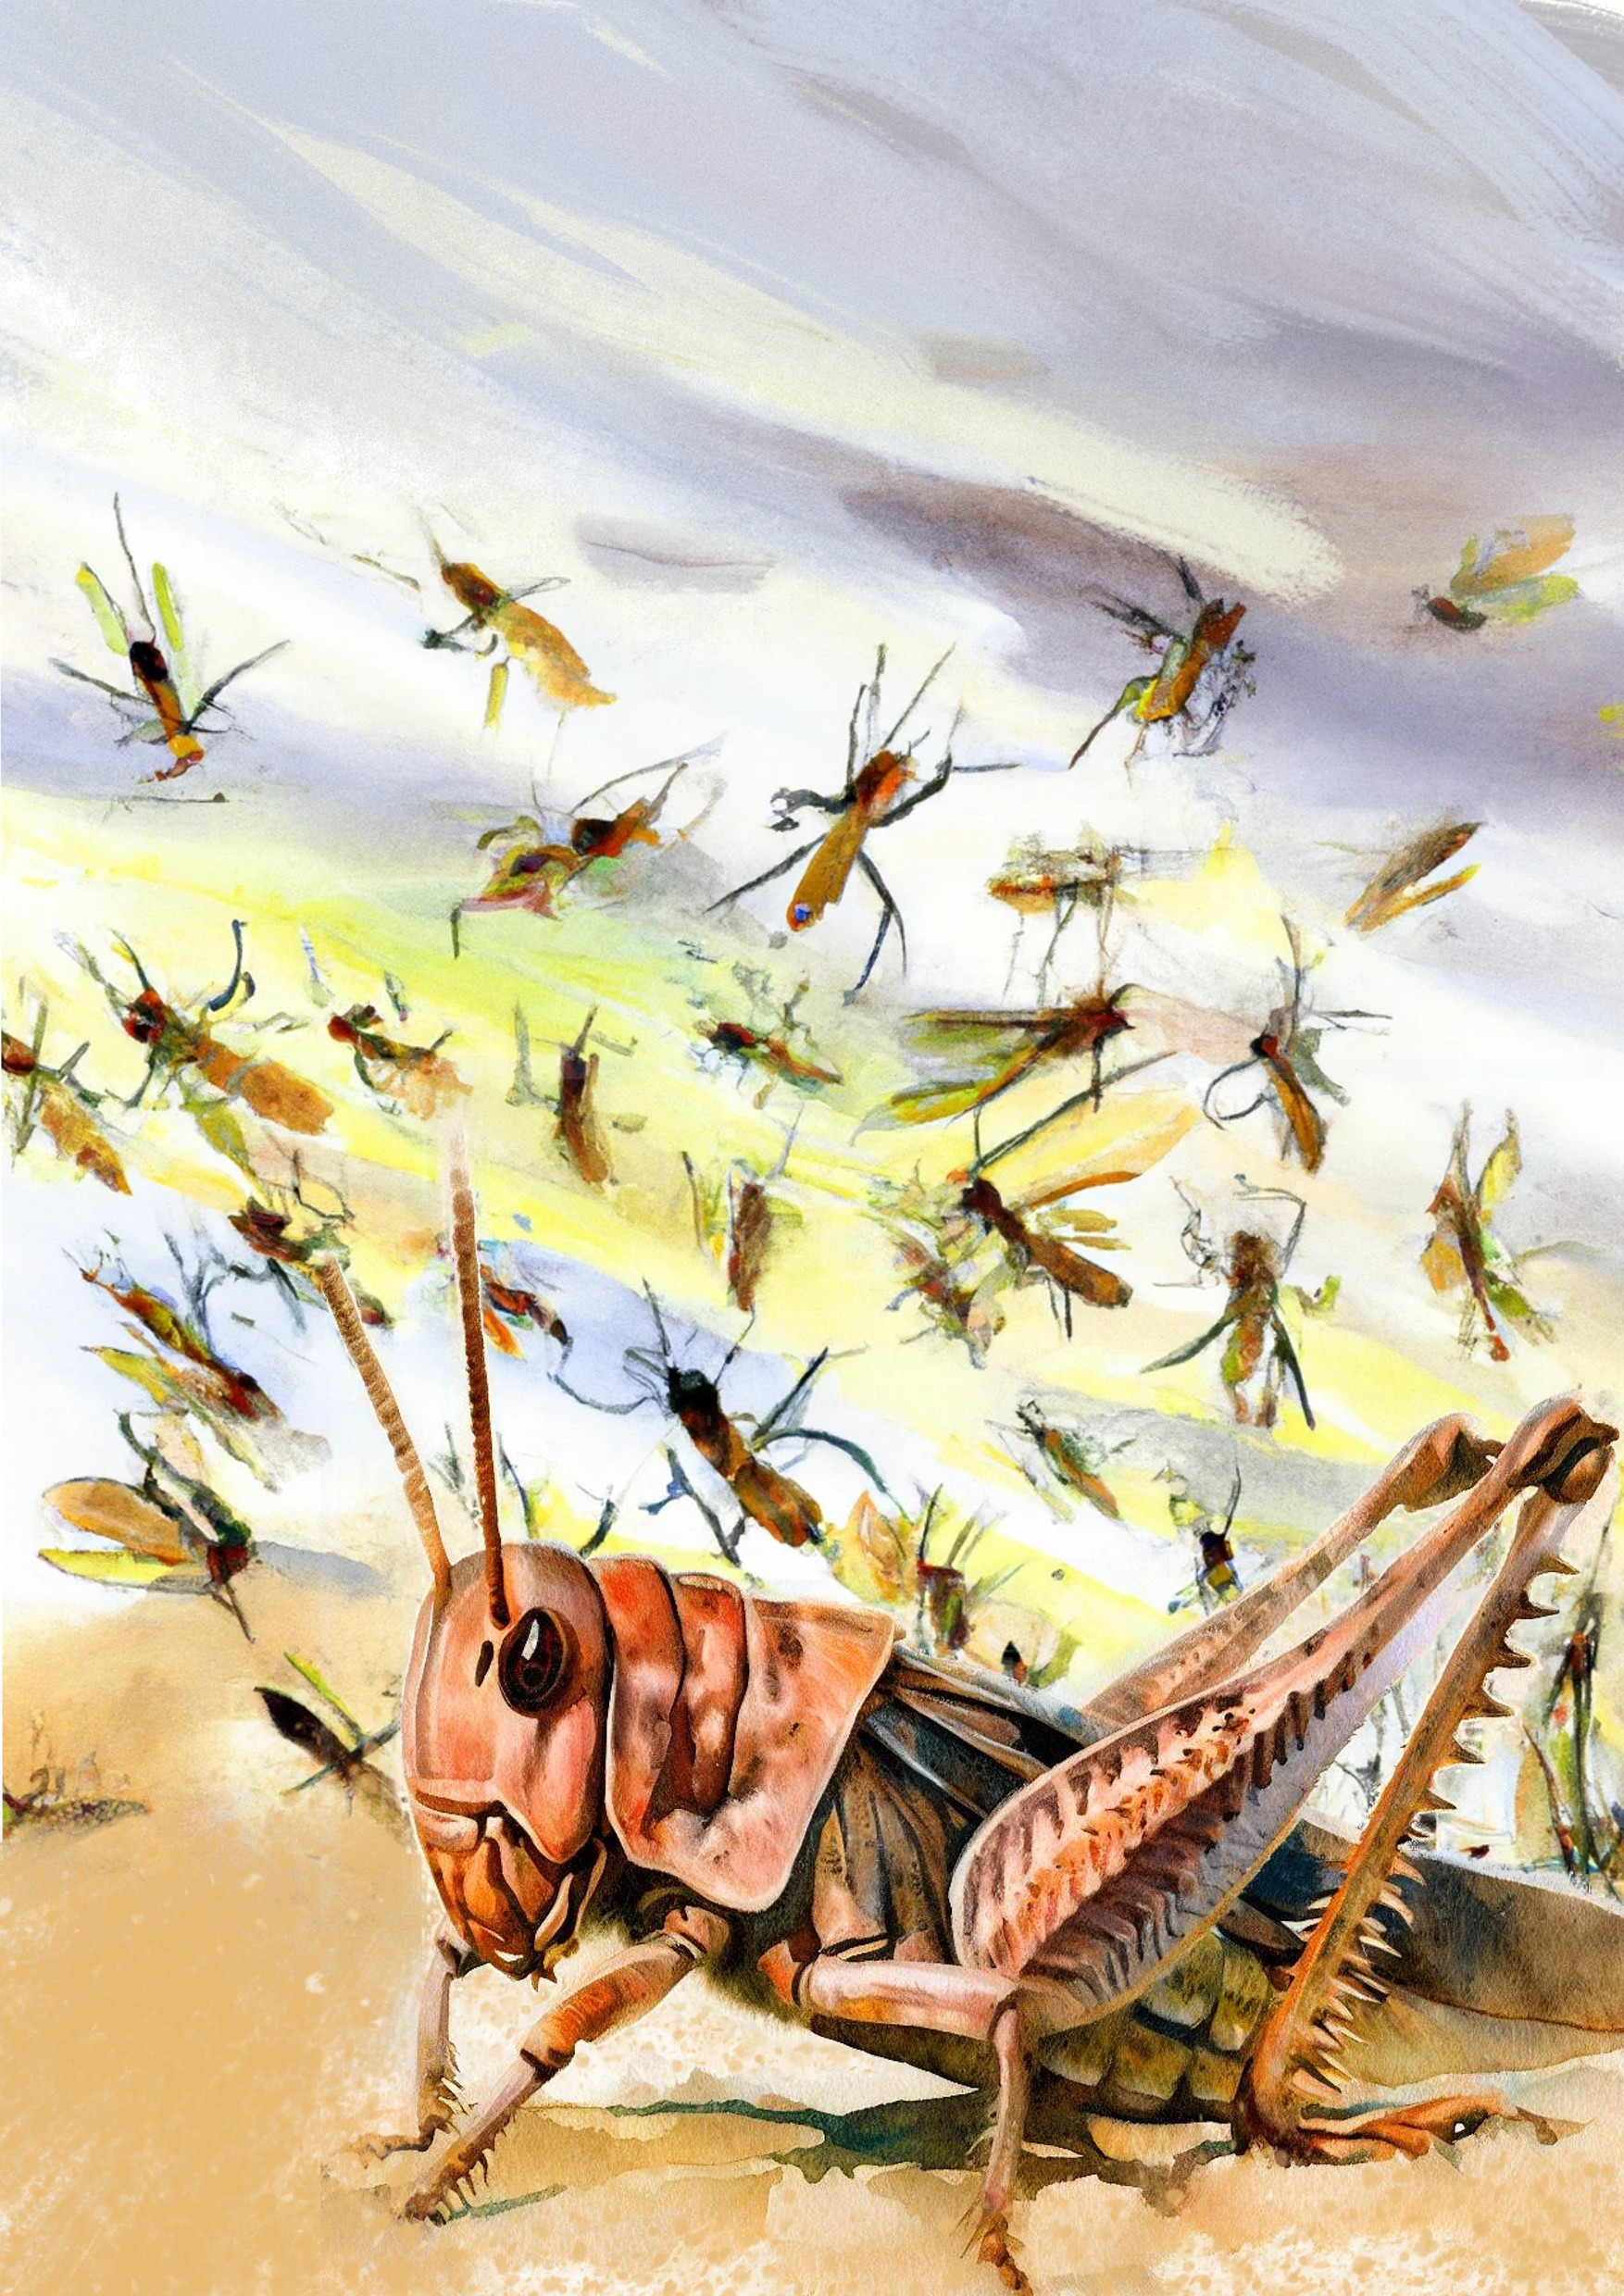
\includegraphics[width = \paperwidth, height = \paperheight] {images/locust-focus}}}
\BgThispage
\newpage

\newpage
\hfill
\backgroundsetup{scale = 1, angle = 0, opacity = 1, contents = {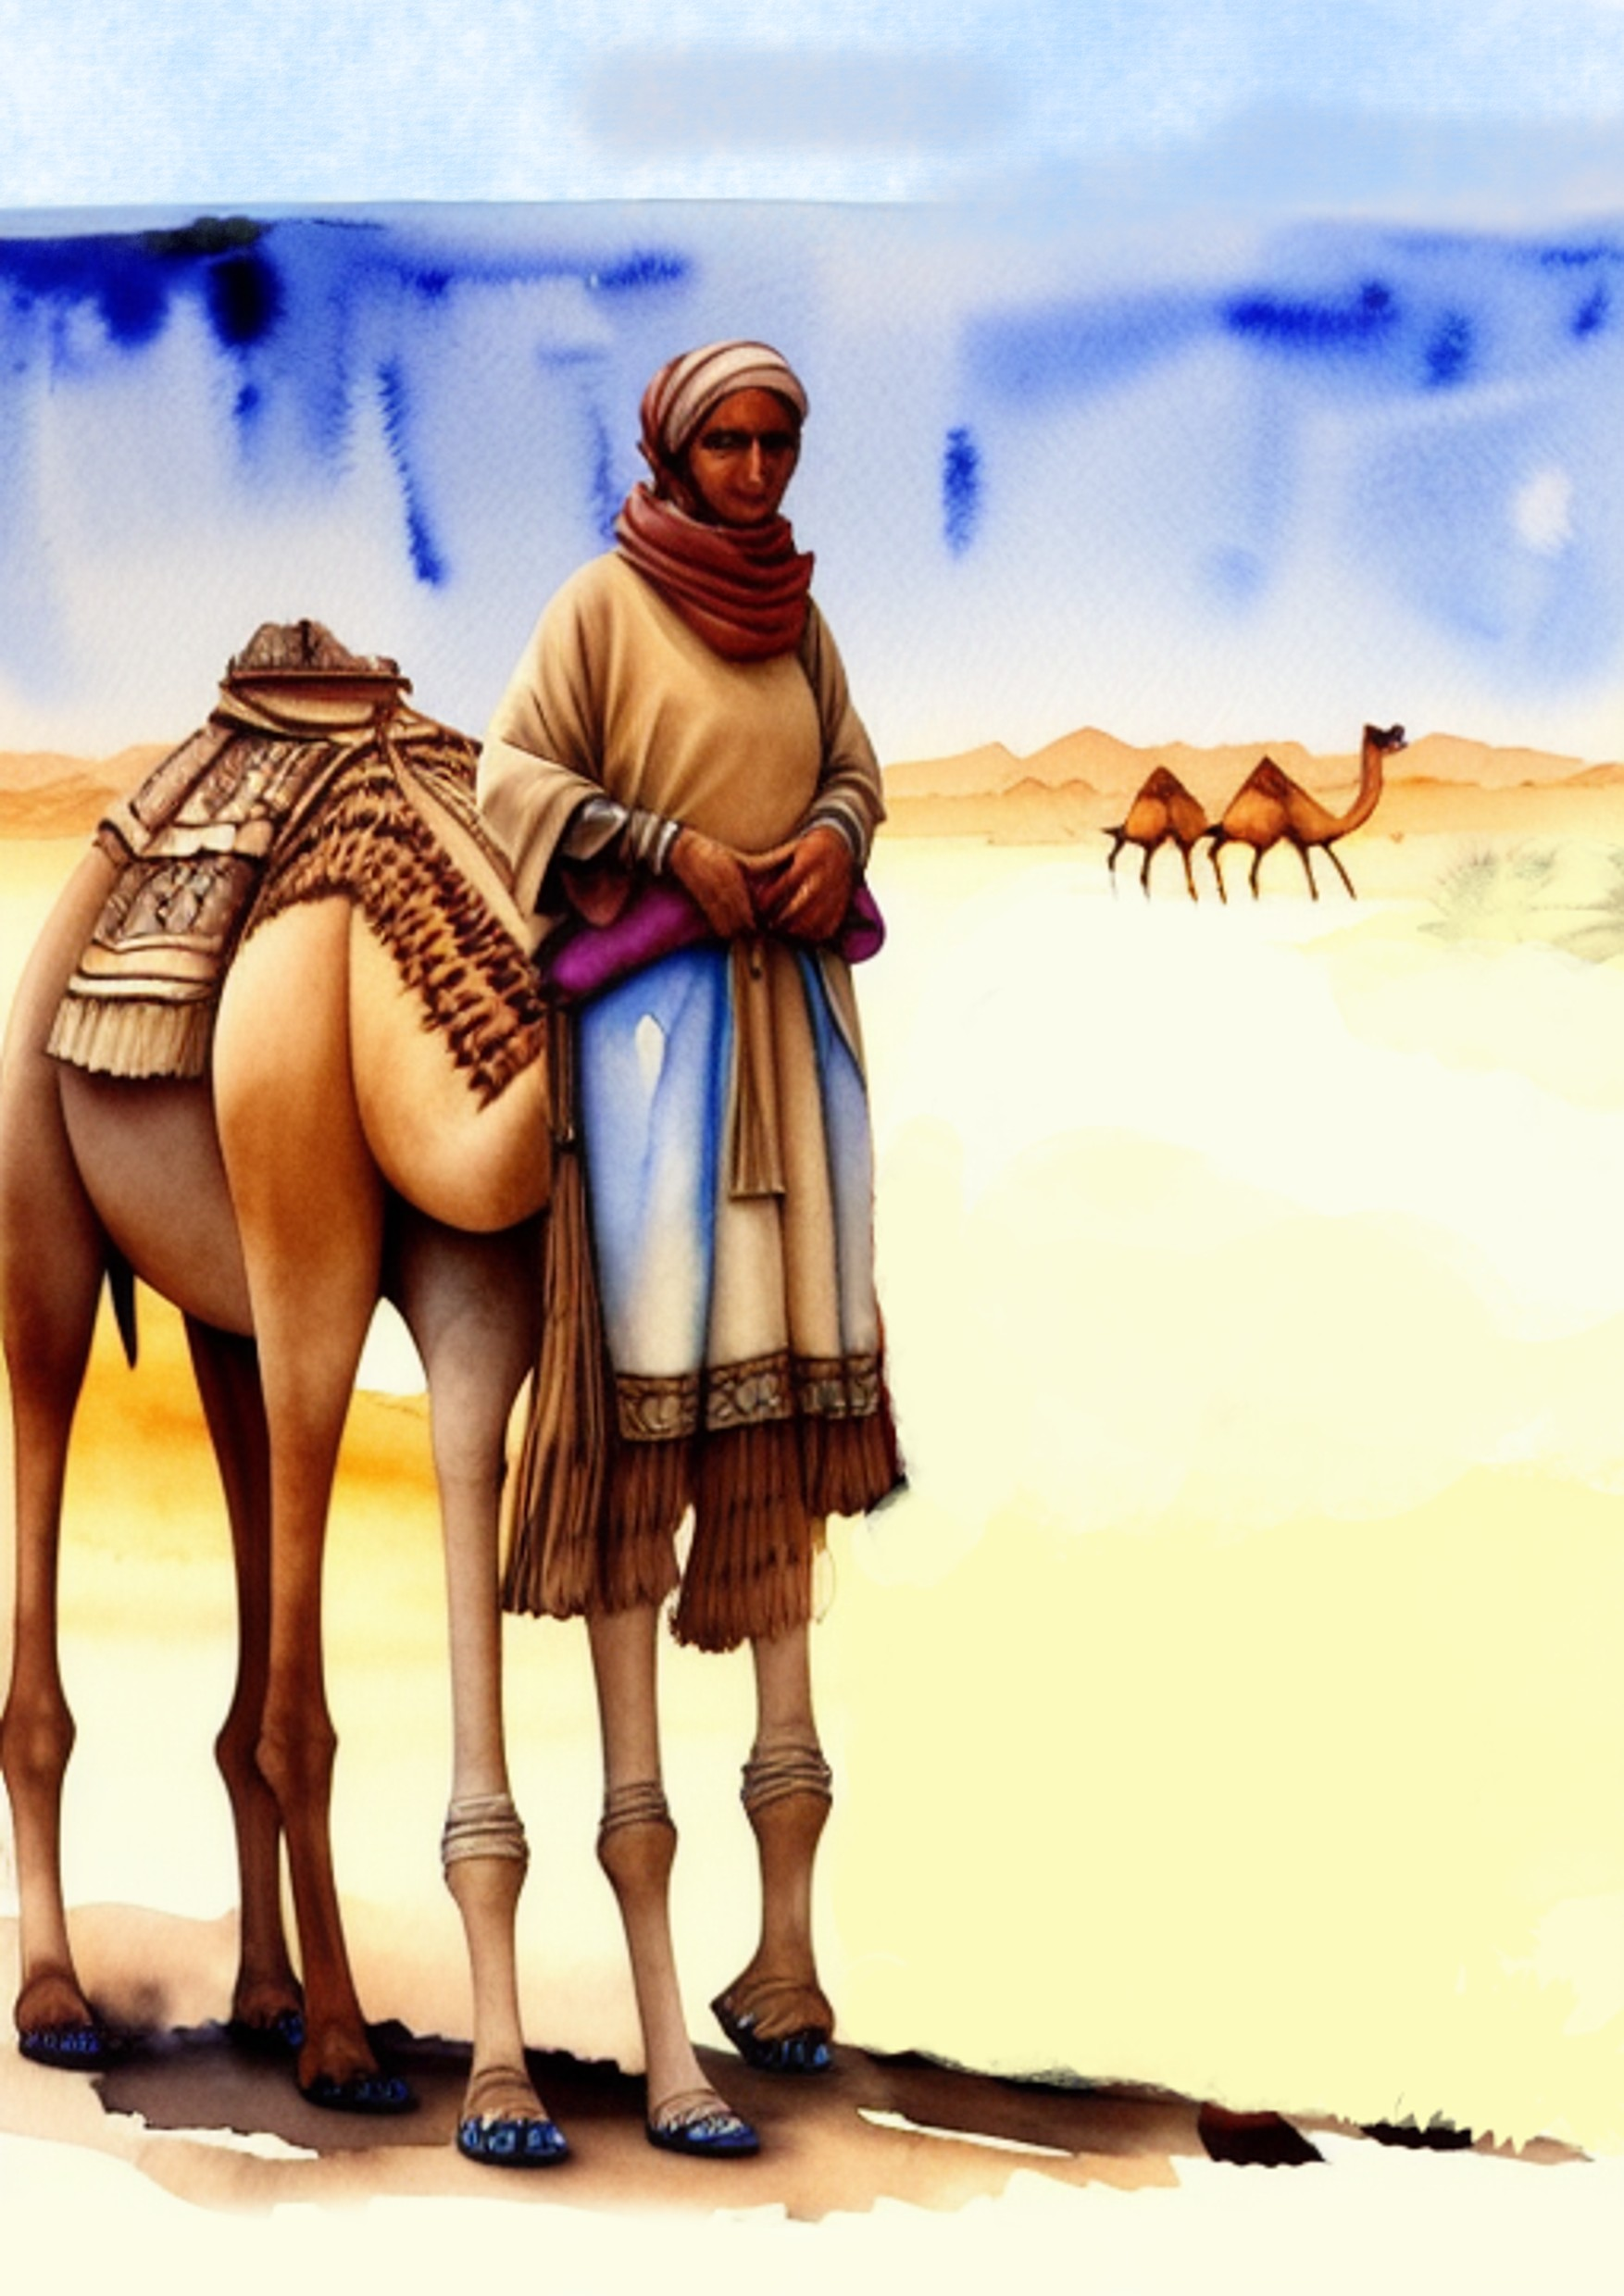
\includegraphics[width = \paperwidth, height = \paperheight] {images/camelhuman}}}
\BgThispage
\newpage

\newpage
\begin{figure}[h]
  \centering
  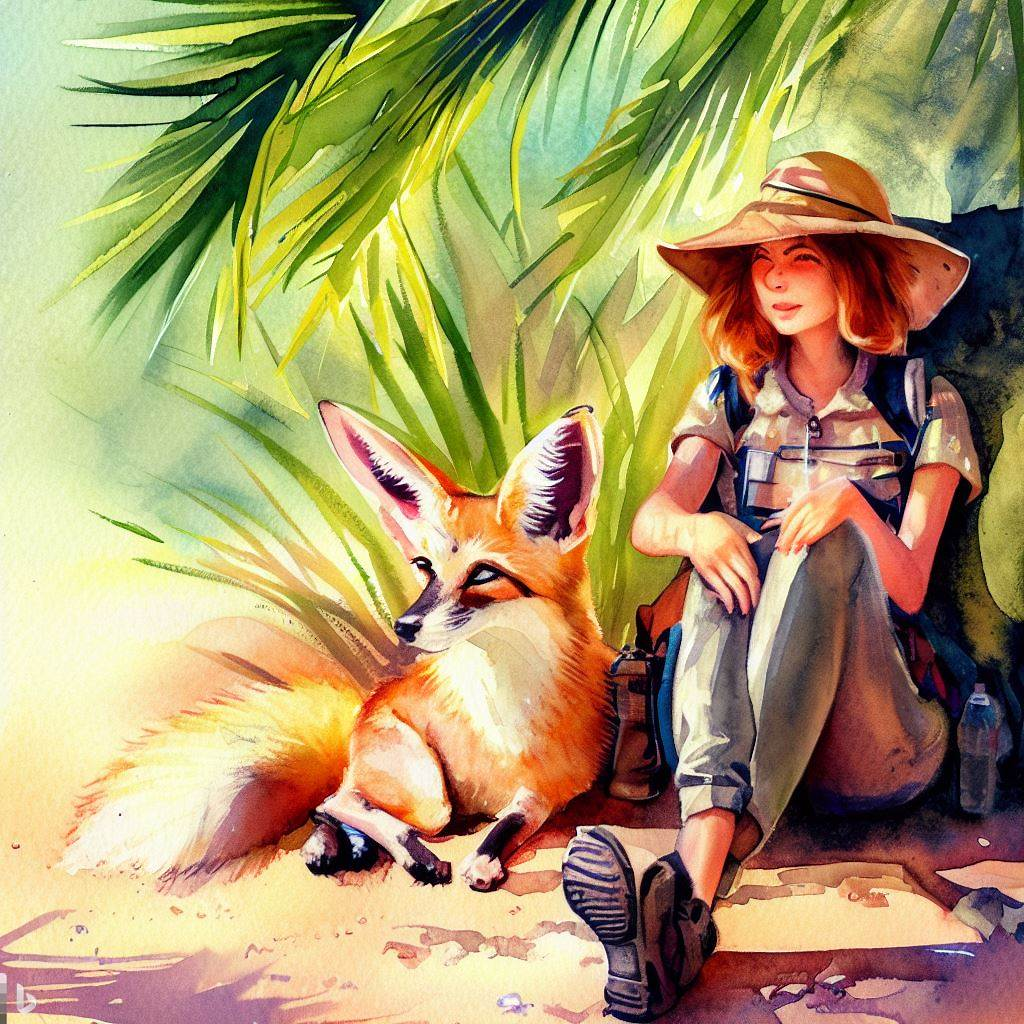
\includegraphics[width=0.55\textwidth]{images/oasis-break.jpg}
  \caption{Отдых в тени пальмы}
\end{figure}

% \vspace{-1cm}

\begin{figure}[h]
  \centering
  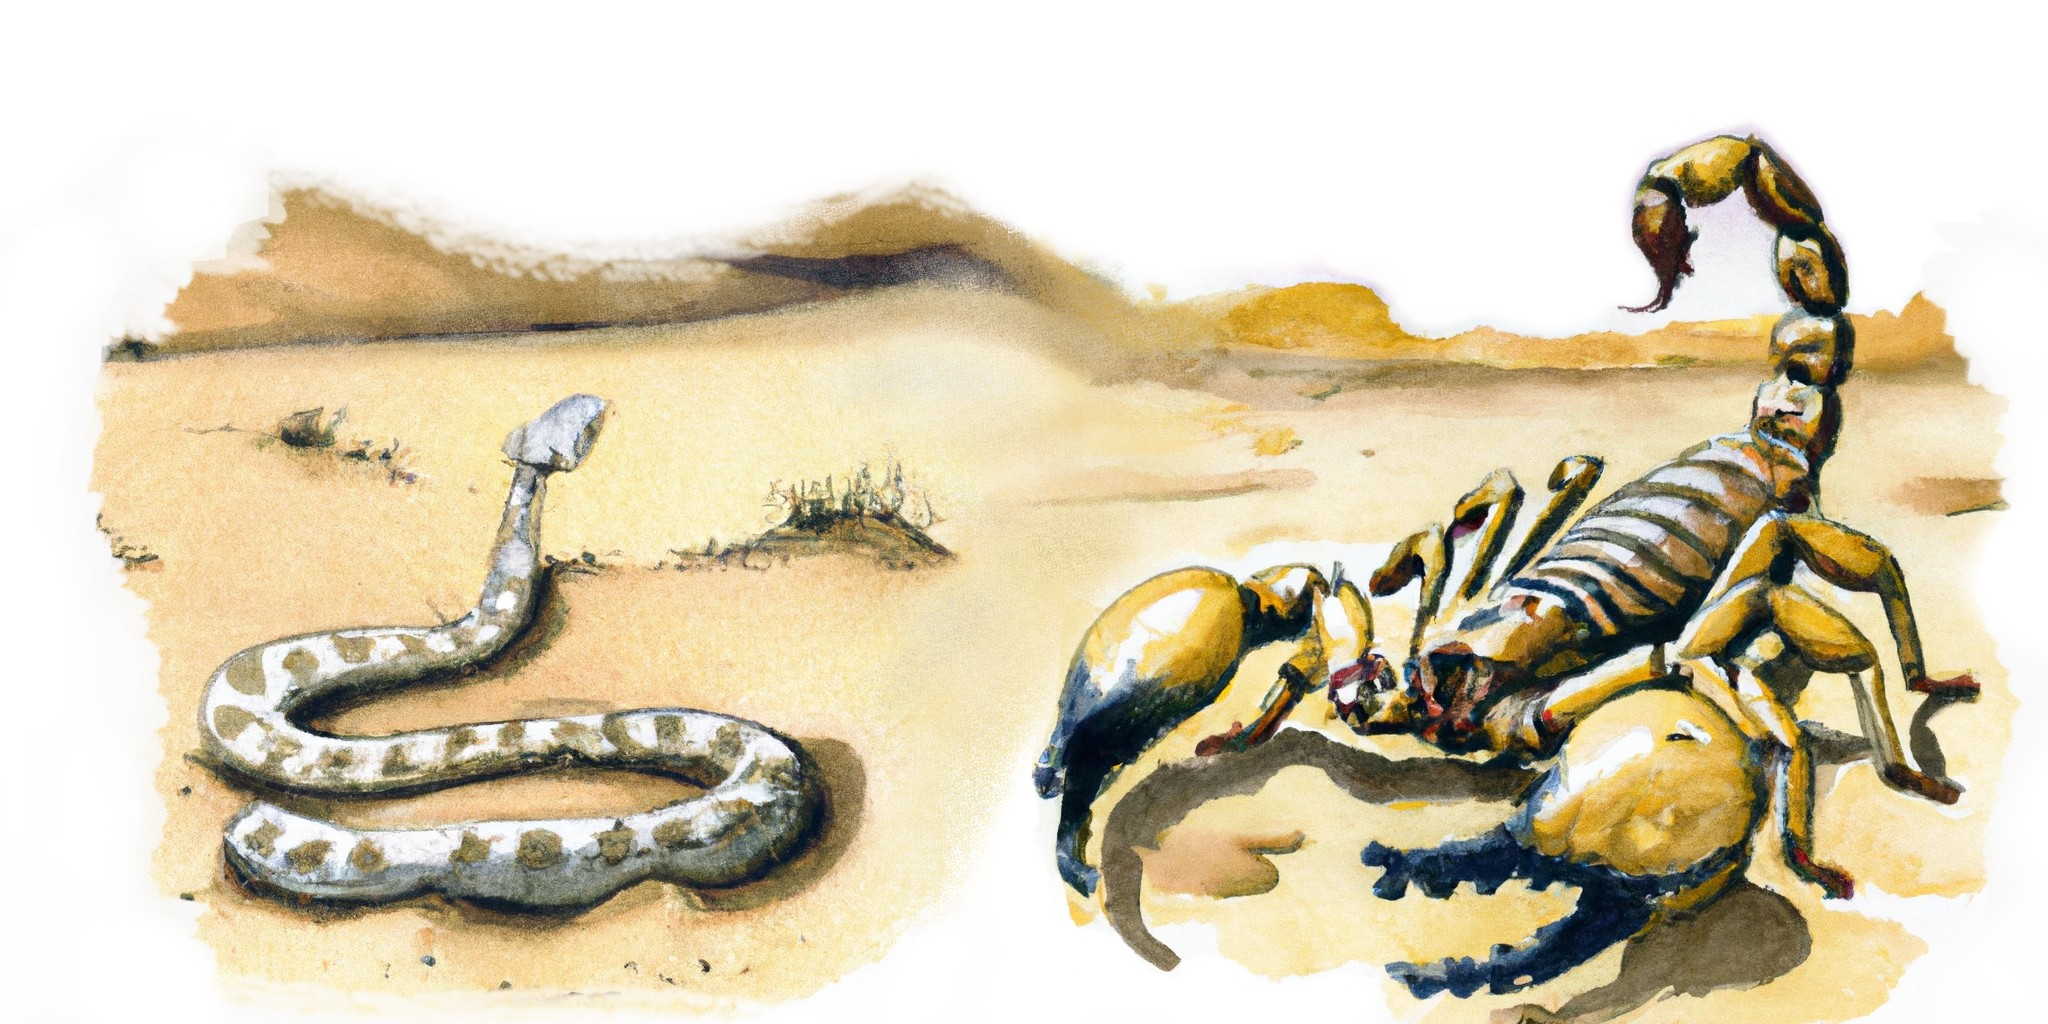
\includegraphics[width=\textwidth]{images/viper-scorpion.jpg}
  \caption{Гадюка и скорпион}
\end{figure}


\newpage
\hfill
\backgroundsetup{scale = 1, angle = 0, opacity = 1, contents = {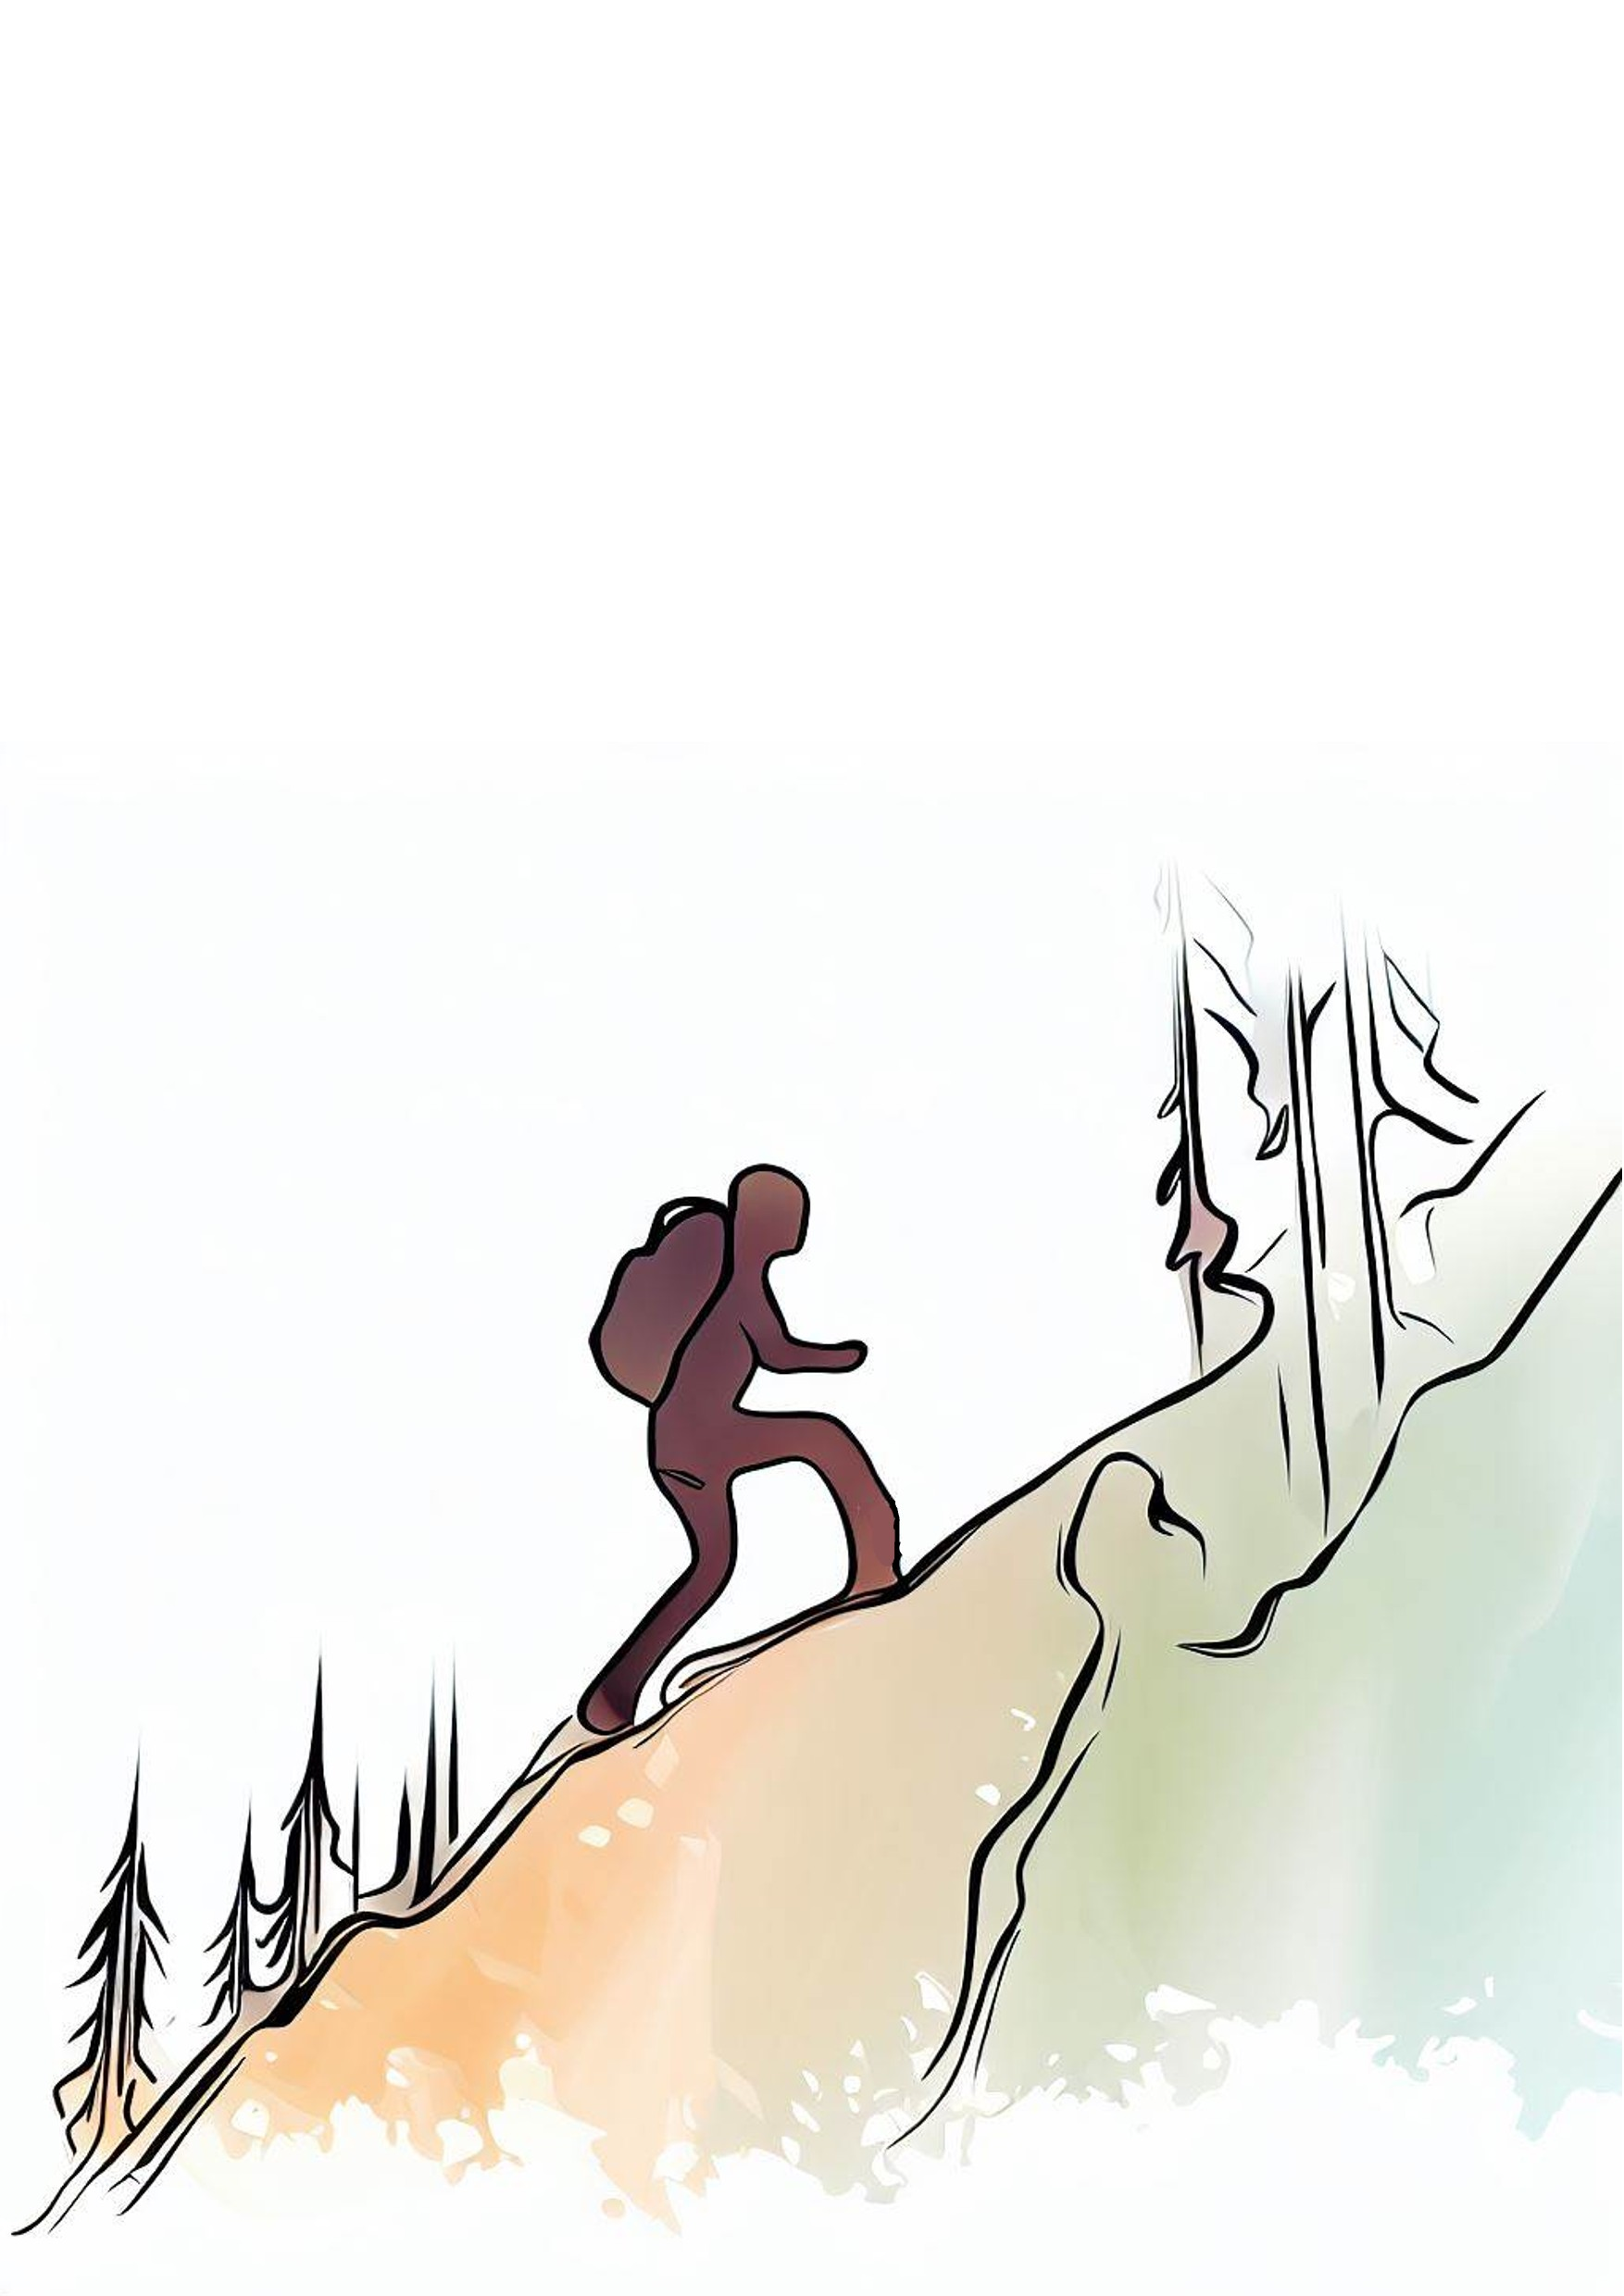
\includegraphics[width = \paperwidth, height = \paperheight] {images/climber.jpg}}}
\BgThispage


\newpage
\PlainPoemTitle
\PoemTitle{Сила воли}
\vspace{2cm}
\begin{verse}[\versewidth]
\hspace{1.5cm}Среди сил безграничной Вселенной, \\
\hspace{1.5cm}меж туманностей, звёзд и планет, \\
\hspace{1.5cm}мощнейшая сила таится --- \\ 
\hspace{1.5cm}о ней я раскрою секрет.
\end{verse}

\begin{verse}[\versewidth]
\hspace{1.5cm}Это сила собственной воли! \\
\hspace{1.5cm}Подвластна она лишь тебе, \\
\hspace{1.5cm}её никто, никогда не отнимет, \\
\hspace{1.5cm}она действует всегда и везде.
\end{verse}

\begin{verse}[\versewidth]
\hspace{1.5cm}Стоит всего-лишь подумать, \\
\hspace{1.5cm}стоит всего захотеть, \\
\hspace{1.5cm}если добавить усилий --- \\ 
\hspace{1.5cm}откроется каждая дверь!
\end{verse}

\begin{verse}[\versewidth]
\hspace{1.5cm}Щёлкнет любой выключатель, \\
\hspace{1.5cm}мигом найдутся носки, \\
\hspace{1.5cm}яблоко будет в тарелке, \\
\hspace{1.5cm}преграды исчезнут с пути!
\end{verse}

\begin{verse}[\versewidth]
\hspace{1.5cm}Ты можешь сама выбрать книгу, \\
\hspace{1.5cm}ты можешь игрушку достать, \\
\hspace{1cm}из блоков ты можешь как хочешь --- \\
\hspace{1cm}башни и замки создать!
\end{verse}


\begin{verse}[\versewidth]
Нужно всего-лишь не сдаться, \\
нужно всего-лишь начать. \\
\textbf{Если добавить усилий, \\
помехи начнут отступать}.
\end{verse}

\backgroundsetup{scale = 1, angle = 0, opacity = 1, contents = {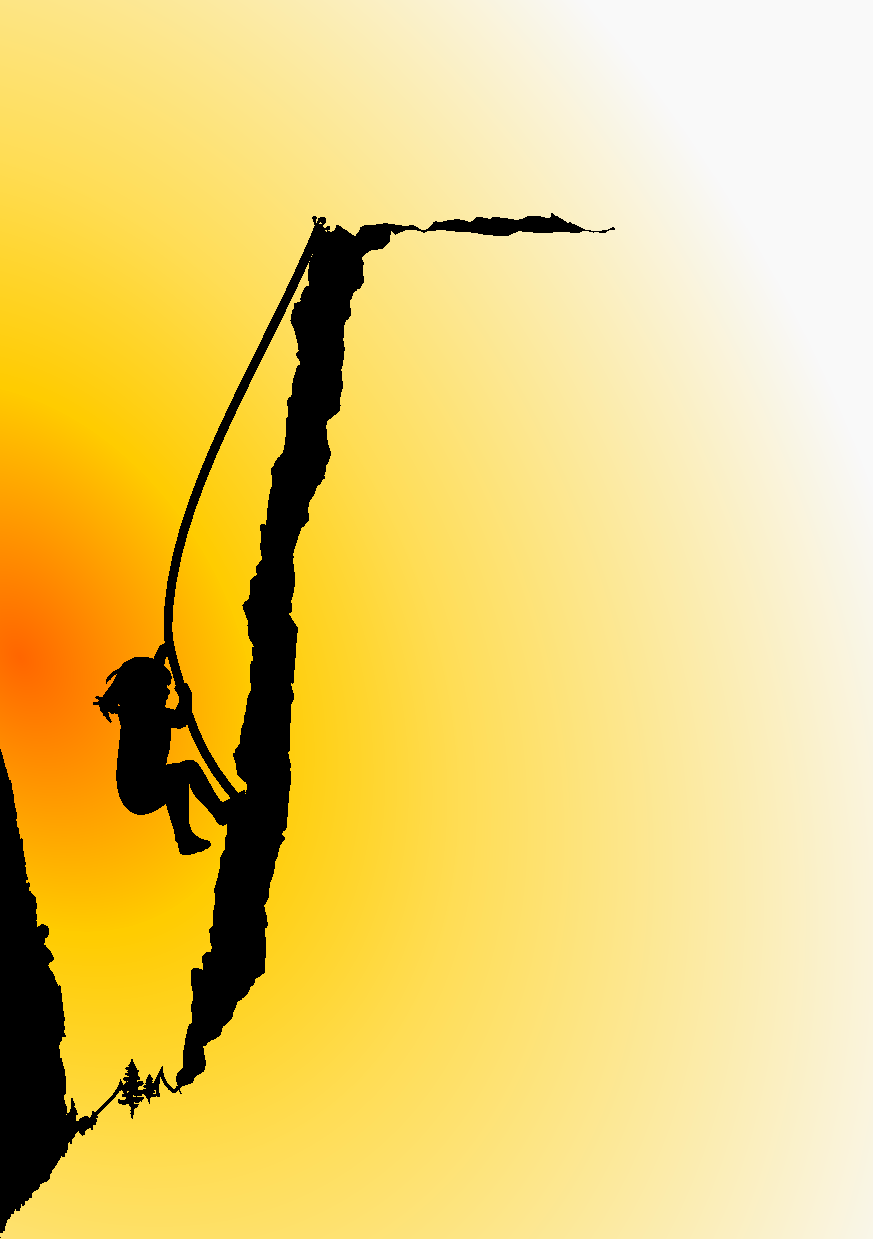
\includegraphics[width = \paperwidth, height = \paperheight] {images/childclimbing}}}
\BgThispage

\newpage

\PlainPoemTitle
\PoemTitle{Шиничи и Синица}
\settowidth{\versewidth}{ступеньки под весом скрипят и трещат ---}
\begin{verse}[\versewidth]
Щенок Шиничи, и Птица-Синица\\
решили в Токио водицей напиться.\\
Под ветками сакуры они прогулялись\\
сквозь толпы туристов еле пробрались.\\
Дошли до фонтана, хвостами махнули\\
и чистой кристальной водицы глотнули.\\
\end{verse}
% ***

\begin{verse}[\versewidth]
\say{Слушай, Шиничи}, сказала синица,\\
\say{Что там за буквы на красной таблице?}\\
\say{Не знаю, сестрица, я должен признать \\
Что не умею пока-что читать\ldots} \\
\end{verse}

\begin{verse}[\versewidth]
\say{Кстати, синица, почему у тебя \\
Вместо перьев на макушке рога?} \\
\say{Быть так не может, синица ведь птица!\\ 
У птиц нет рогов --- тебе это снится!} \\
\end{verse}

\begin{verse}[\versewidth]
\say{Кстати, Шиничи, может мне тоже снится,\\ 
Но почему у тебя вместо ножек копытца?} \\
\say{Копытца? Как так? Не бывает копыт у собак!}\\
\end{verse}

\begin{verse}[\versewidth]
\say{Карр-карр}, прервала их ворона\\
Спустившись с верхушки зелёного клёна.\\ 
\say{Ребятки, должна вас прервать\\
И срочно таблицу для вас прочитать.}\\ 
\end{verse}

\begin{verse}[\versewidth]
\say{Тут говорится, на трех языках, \\
Жёлтым по красному, в громких тонах:\\
Фонтан заколдован! Не пей, а иначе \\
Козлёночком станешь, потеряешь удачу!} 
\end{verse}

\begin{verse}[\versewidth]
Испугались щенок и синица, \\
Страхом мгновенно покрылись их лица! \\
Плачет синица, рыдает щенок\ldots \\
\say{Что теперь делать? Кто 'б нам помог?} 
\end{verse}





% \backgroundsetup{contents=Bazaar,color=green}
% \BgThispage 

% add a blank page here so the addendum has its own spread
\clearpage
\hfill
\clearpage
\section*{Родителям на заметку}
\addcontentsline{toc}{section}{Родителям на заметку}


\begin{description}

\item[Хакатон] От английского hacker + marathon, событие которое собирает разных энтузиастов (программисты, графические дизайнеры, итд.) для совместной разработки решения некой проблемы. 
\fancybreak{*}

\item[Улур\'{у}] Гора в Австралии, которую коренные жители континента считают священной (cтр.~\pageref{uluru}).

\item[Вомб\'{а}т] Вид животных обитающих  в Австралии. Представь себе хомяка весом \textasciitilde30кг.
\begin{center}
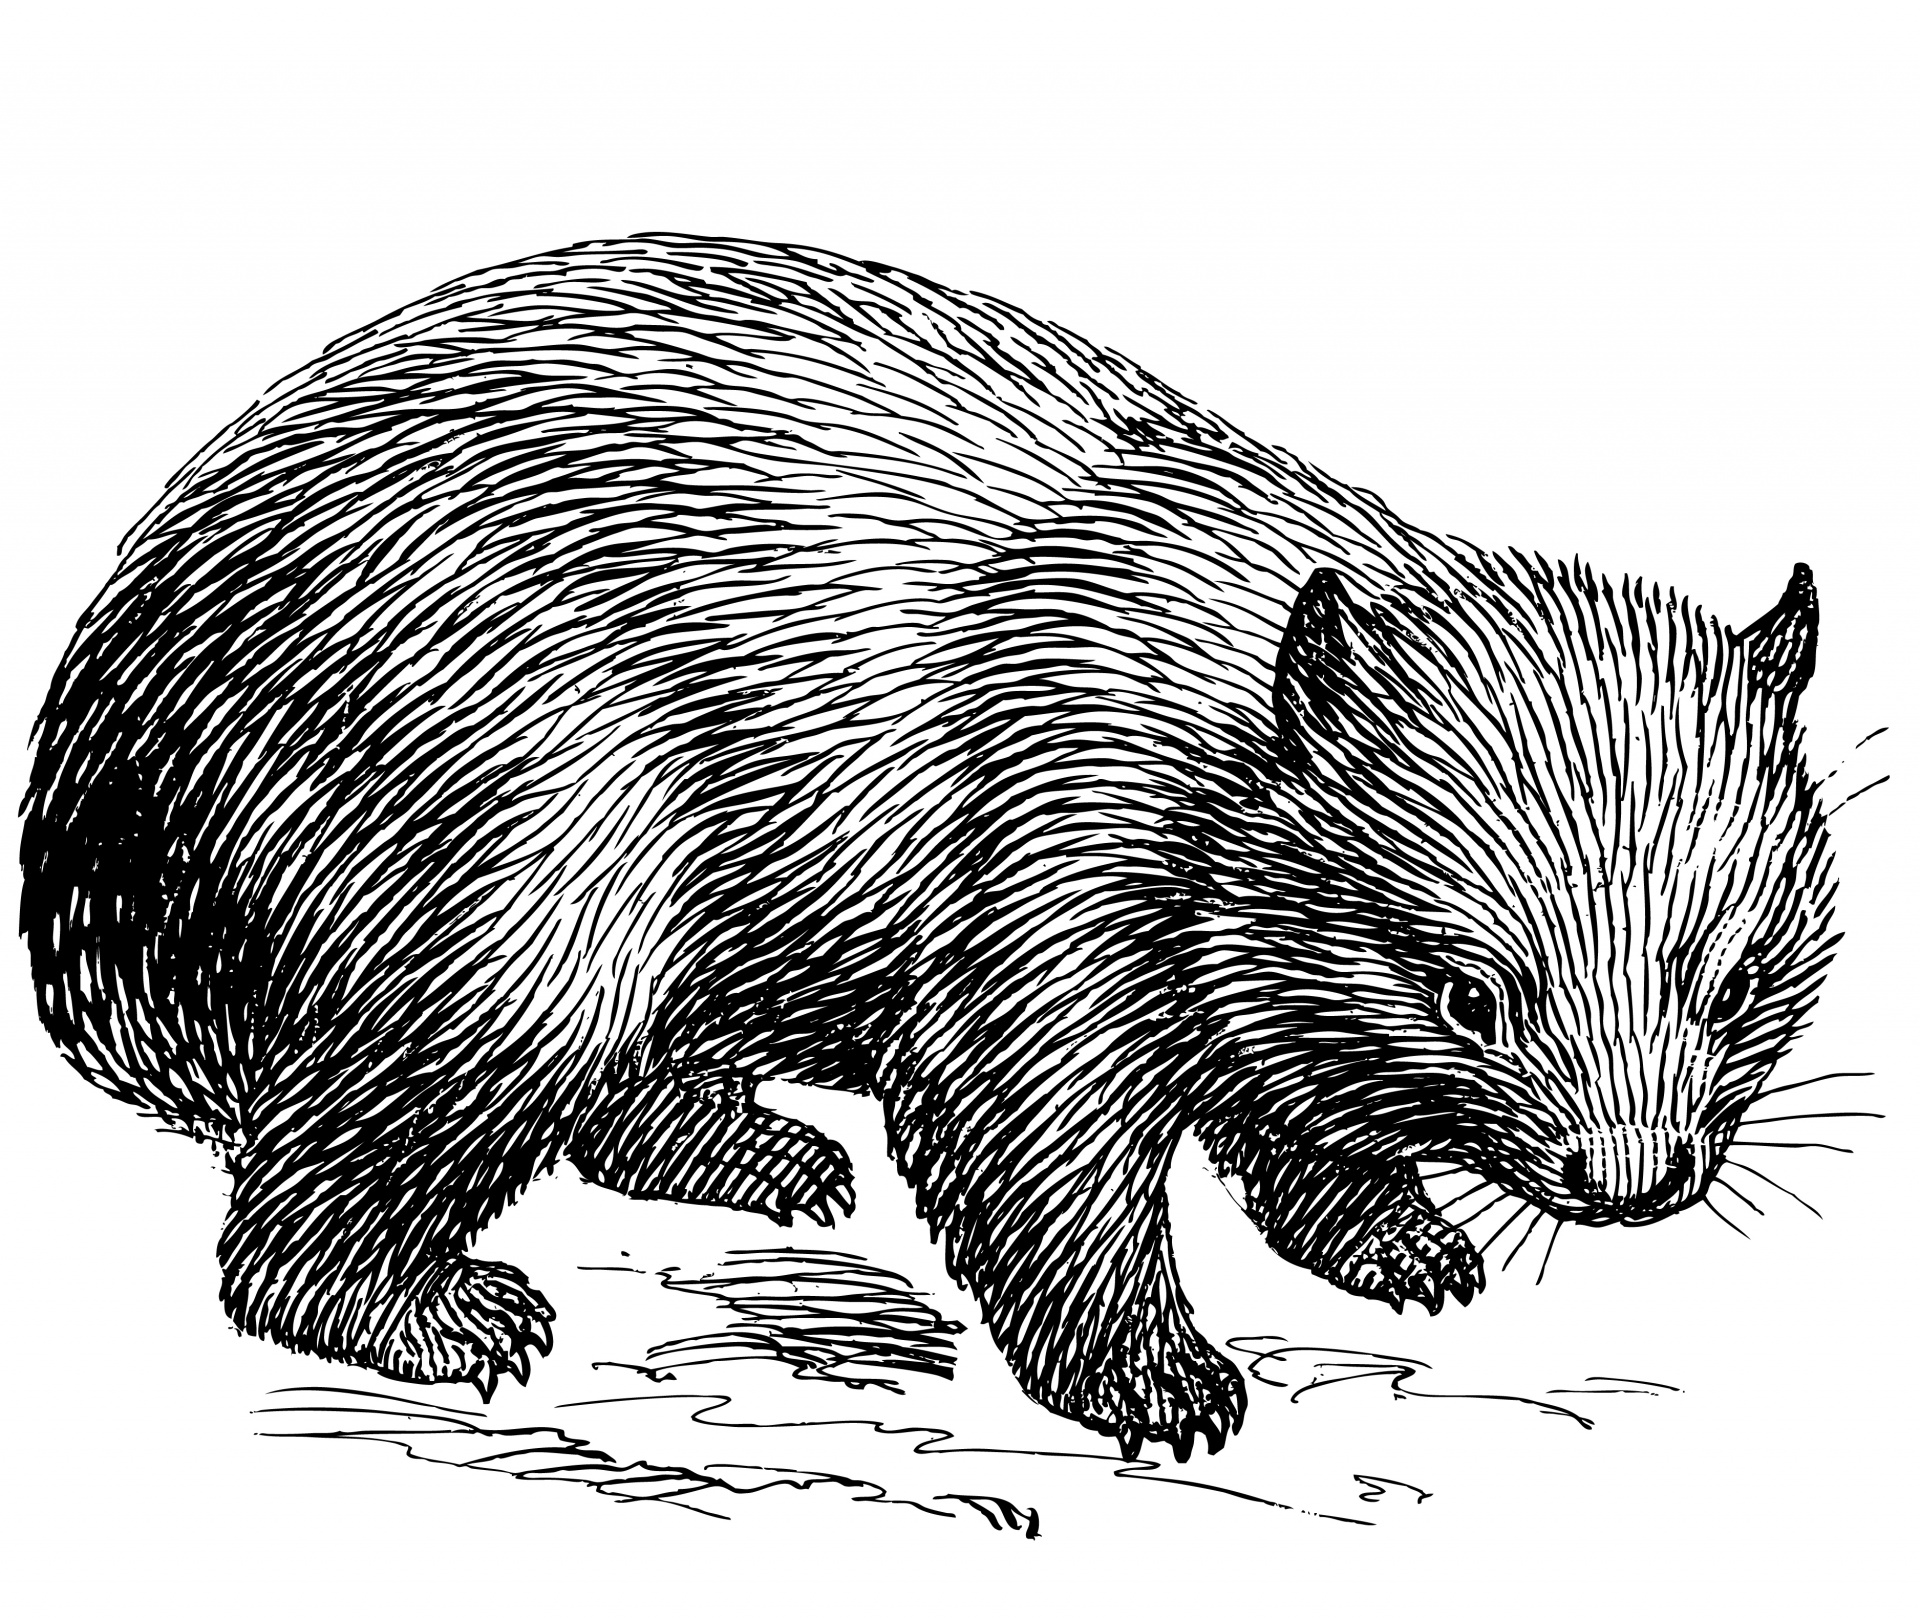
\includegraphics[height=4cm]{images/wombat} 
\end{center}

\item[Диджериду] Музыкальный инструмент австралийских аборигенов. Для примера, можно послушать ``David Hudson - Rainbow Serpent''. 

\item[\textquote{По теченью Пути}] Речь о нашей галактике -- Млечный Путь. Если посмотреть на ночное небо вдали от цивилизации и источников света, можно наблюдать что-то похожее на иллюстрацию на стр.~\pageref{milky-way} - боковой вид нашей галактики изнутри.

\item[Сверхнова] Сверхновая звезда -- заключающая фаза цикла жизни некоторых звёзд, в результате которой выделяется очень много энергии. Взрыв разбрасывает большое количество материи в пространство, при этом наблюдается очень яркая вспышка. Внимание, свехрновы лучше наблюдать издалека! Деструктивный потенциал этого явления может уничтожить любые формы жизни в отдельном регионе космоса. 
\fancybreak{*}

\item[Кинцуги] Японская традиция реставрации разбитой керамики. Мыцумото адепт этой идеи. Он считает что поломки и трещины -- часть жизни, и они составляют важную часть истории каждого из нас.

\item[Стоицизм] Жизненный подход Лао Вэнга.
``Our life is what our thoughts make it'' and ``It's not what happens to you, but how you react to it that matters''.
\fancybreak{*}

\item[Сафари] На арабском языке это означает \textquote{путешествие}.

\item[Туар\'{е}ги] Кочевой народ проживающий на севере Африки, например в Алжире или Ливии. Традиционный наряд туарегов включает вещи цвета индиго (что-то между тёмно-синим и фиолетовым).


\item[Ф\'{е}нек] Маленькая лиса с большими ушами, обитает в пустынях на севере Африки. Имя происходит от арабского \textquote{фанак}, что означает \textquote{лиса}. 


\item[В\'{а}ди] В арабском языке, это русло высохшей реки. Иногда они могут временно заполняться после проливных дождей.

\item[Космо--хоровод] Если фотографировать ночное небо с достаточно длительной выдержкой, прицелившись на Полярную звезду, можно заметить округленный след звёзд, который формируется за счёт вращения Земли вокруг своей оси.

% https://youtu.be/4yFaMsUawi4
\item[Поющие пески] Этот феномен можно наблюдать в сухую погоду, перемещаясь по поверхности дюн. Для примера, найди видео ``Mathias Th\'ery - The song of the dunes''.
\end{description}



% adjust this horizontal offset as needed
% \hspace{-6.35cm}
% \includegraphics[width=\paperwidth]{images/sahara-stars-annotated.png} 


\clearpage
\subsection{Как распечатать эту книгу?}

\renewcommand{\thefootnote}{\fnsymbol{footnote}}

\begin{enumerate}
    \item Нужен принтер с опцией двусторонней печати.
    \item Открыть файл PDF в Adobe Acrobat Reader (именно в нём!).
    \item В меню \menu{Файл > Печать} (или \keys{\ctrl + P}) нажать на кнопку \menu{Booklet}.
    \item Согнуть\footnote[2]{Внимание! Вынимая бумагу из принтера, помни, что она может быть горячей! Настоятельно рекомендуется применение митрилловых перчаток!} страницы \emph{как есть}, они уже в нужном порядке.
    \item Закрепить степлером, вставить скобы вручную, или сшить.
\end{enumerate}

\subsection{Как адаптировать эту книгу?}
Для личных, внутрисемейных целей, например: если вы хотите поменять размер листа, увеличить шрифт, или заменить слона Харитона на изображение любимого слона вашего ребёнка -- редактируйте эту книгу используя исходный код  \href{https://github.com/ralienpp/book-one}{github.com/ralienpp/book-one}.

В творческом процессе применялись эти инструменты: Inkscape, Krita, GIMP, Paint.NET, Stellarium, Sketchbook, StableDiffusion, Dall-E, \LaTeX. Если вы с ними не знакомы, и если попытки импровизировать не дали результат -- воспользуйтесь опцией ``Github issues'' чтобы попросить о помощи.

Если ваши изменения являются общими улучшениями, которые могут быть полезны другим читателям -- откройте ``pull request'', чтобы сделать их частью проекта.

Книга распространяется по лицензии \href{https://creativecommons.org/licenses/by-sa/4.0/}{CC-BY-SA}.


\clearpage
\section*{English translations}
\addcontentsline{toc}{section}{English translations}
These translations are here to give you an idea of what this book is about. They were generated by ChatGPT and slightly tweaked to improve rhyme and rhythm.


\PlainPoemTitle
\PoemTitle*{Willpower}
\begin{multicols}{2}


\begin{verse}[\versewidth]
Amid the forces of the Universe,\\
Among nebulae, stars, and planets,\\
There lies a mighty force concealed\\
Its secret I shall now reveal.
\end{verse}

\begin{verse}[\versewidth]
It is the power of your will!\\
Subjected just to your command,\\
No one can take it away from you,\\
It acts always and everywhere.
\end{verse}

\begin{verse}[\versewidth]
Just think of it, just wish for it,\\
Then add an effort to your thought,\\
And every door will open wide,\\
For you to achieve what you sought!
\end{verse}


\begin{verse}[\versewidth]
Switches will flip in a snap,\\
Socks will be found in a trice,\\
An apple will be on your plate,\\
Obstacles vanish from sight!
\end{verse}

\begin{verse}[\versewidth]
You can grab any book from a shelf,\\
You can easily reach any toy,\\
With blocks you can create at will\\
Castles and towers to enjoy!
\end{verse}

\begin{verse}[\versewidth]
All you need is to persist,\\
All you need is to begin,\\
If you add some extra zeal,\\
Obstacles will soon give in!
\end{verse}


\end{multicols}

% this is the back-cover of the book
\cleartoverso
% \cleartoevenpage
% \clearpage
\thispagestyle{empty}  % to not have a page# here


\section*{Другие книги нашего издательства}
% \vspace{2cm}

\begin{table}[h]
\begin{tabular}{ccc}
\includegraphics[height=4cm]{images/lisa-v-lesu} & \includegraphics[height=4cm]{images/yak-kayak} & \includegraphics[height=4cm]{images/dog-book-cooker}             \\
 Лиса в лесу    &  Я, як, и каяк        &   Собака, которая            \\
  нашла косу &  & любила цифры \\
            &          &              \\
\includegraphics[height=4cm]{images/magic-pyramid} & \includegraphics[height=4cm]{images/cave-stories} & \includegraphics[height=4cm]{images/razukrashki.jpg}             \\
 На плечах гигантов       &  Волшебная пещера    &     Разукрашки \\    
        &      &     Дваукрашки \\
        &      &     Триукрашки \\
\end{tabular}
\end{table}

\subsection{Автор и обратная связь}
\hspace{-1cm}
\noindent
\begin{tabular}{p{12cm}p{2cm}}
\footnotesize{Этот сборник стихов из частично-восстановленного архива, найденного среди развалин архаического вычислительного центра, на дне озера $0x\Sigma \alpha \phi^4_5\bigoplus$. Исходя из метаданных, стихи были написаны в первой половине XXI века Ручной эпохи Досингулярной эры. Предполагаемое имя автора Papa de la M{\"u}nchen, или Папа де ла Мюнхен, или Папа Мюнхенксий (возможно искажение транслитерации). % Среди блоков данных был найден и фрагмент который не поддавался текстовой интерпретации, мы прилагаем его в виде двухмерной монохромной матрицы. Остальные двухмерные матрицы в сборнике были сгенерированны нами, исходя из контекста.
О неточностях и ошибках сообщайте в Департамент Интерпретаций: alex\Dolphin{}railean.net.} & \hspace{-5mm}\raisebox{-2.2cm}{ \includegraphics[height=2.5cm]{images/maskavatar-trimmed.jpg}}
\end{tabular}



% \begin{wrapfigure}{r}{8cm}
% % \begin{wrapfigure}[10]{r}{0.08\textwidth}
% \vspace{-0.5cm}
% \centering
% \includegraphics[height=2.7cm]{images/maskavatar-trimmed.jpg}
% % \vspace{-110pt}
% % \rule{3cm}{2cm}
% \end{wrapfigure}

% \footnotesize{Этот сборник стихов из частично-восстановленного архива, найденного среди развалин архаического вычислительного центра, на дне озера $0x\Sigma \alpha \phi^4_5\bigoplus$. Исходя из метаданных, стихи были написаны в первой половине XXI века Ручной эпохи Досингулярной эры. Предполагаемое имя автора Papa de la M{\"u}nchen, или Папа де ла Мюнхен, или Папа Мюнхенксий (возможно искажение транслитерации). % Среди блоков данных был найден и фрагмент который не поддавался текстовой интерпретации, мы прилагаем его в виде двухмерной монохромной матрицы. Остальные двухмерные матрицы в сборнике были сгенерированны нами, исходя из контекста.
% О неточностях и ошибках сообщайте в Департамент Интерпретаций: alex\Dolphin{}railean.net.} 


\end{document}


